%% ut-thesis.tex -- document template for graduate theses at UofT
%DIF LATEXDIFF DIFFERENCE FILE
%DIF DEL C:\Users\David\Documents\GitHub\MASc\latex_root_before_committee_rev\ut-thesis.tex   Mon Aug 17 00:25:34 2015
%DIF ADD C:\Users\David\Documents\GitHub\MASc\latex_root\ut-thesis.tex                        Wed Sep  2 13:10:51 2015
%%
%% Copyright (c) 1998-2012 Francois Pitt <fpitt@cs.utoronto.ca>
%% last updated at 09:43 (EDT) on Fri  1 Jun 2012
%%
%% This work may be distributed and/or modified under the conditions of
%% the LaTeX Project Public License, either version 1.3c of this license
%% or (at your option) any later version.
%% The latest version of this license is in
%%     http://www.latex-project.org/lppl.txt
%% and version 1.3c or later is part of all distributions of LaTeX
%% version 2005/12/01 or later.
%%
%% This work has the LPPL maintenance status "maintained".
%%
%% The Current Maintainer of this work is
%% Francois Pitt <fpitt@cs.utoronto.ca>.
%%
%% This work consists of the files listed in the accompanying README.

%% SUMMARY OF FEATURES:
%%
%% All environments, commands, and options provided by the `ut-thesis'
%% class will be described below, at the point where they should appear
%% in the document.  See the file `ut-thesis.cls' for more details.
%%
%% To explicitly set the pagestyle of any blank page inserted with
%% \cleardoublepage, use one of \clearemptydoublepage,
%% \clearplaindoublepage, \clearthesisdoublepage, or
%% \clearstandarddoublepage (to use the style currently in effect).
%%
%% For single-spaced quotes or quotations, use the `longquote' and
%% `longquotation' environments.


%%%%%%%%%%%%         PREAMBLE         %%%%%%%%%%%%

%%  - Default settings format a final copy (single-sided, normal
%%    margins, one-and-a-half-spaced with single-spaced notes).
%%  - For a rough copy (double-sided, normal margins, double-spaced,
%%    with the word "DRAFT" printed at each corner of every page), use
%%    the `draft' option.
%%  - The default global line spacing can be changed with one of the
%%    options `singlespaced', `onehalfspaced', or `doublespaced'.
%%  - Footnotes and marginal notes are all single-spaced by default, but
%%    can be made to have the same spacing as the rest of the document
%%    by using the option `standardspacednotes'.
%%  - The size of the margins can be changed with one of the options:
%%     . `narrowmargins' (1 1/4" left, 3/4" others),
%%     . `normalmargins' (1 1/4" left, 1" others),
%%     . `widemargins' (1 1/4" all),
%%     . `extrawidemargins' (1 1/2" all).
%%  - The pagestyle of "cleared" pages (empty pages inserted in
%%    two-sided documents to put the next page on the right-hand side)
%%    can be set with one of the options `cleardoublepagestyleempty',
%%    `cleardoublepagestyleplain', or `cleardoublepagestylestandard'.
%%  - Any other standard option for the `report' document class can be
%%    used to override the default or draft settings (such as `10pt',
%%    `11pt', `12pt'), and standard LaTeX packages can be used to
%%    further customize the layout and/or formatting of the document.

%% *** Add any desired options. ***
\documentclass{ut-thesis}

%% *** Add \usepackage declarations here. ***
%% The standard packages `geometry' and `setspace' are already loaded by
%% `ut-thesis' -- see their documentation for details of the features
%% they provide.  In particular, you may use the \geometry command here
%% to adjust the margins if none of the ut-thesis options are suitable
%% (see the `geometry' package for details).  You may also use the
%% \setstretch command to set the line spacing to a value other than
%% single, one-and-a-half, or double spaced (see the `setspace' package
%% for details).

\usepackage{amsmath}

\usepackage{graphicx}
\usepackage{caption}
\usepackage{subcaption}

\usepackage{float}
\usepackage{epstopdf}

\usepackage{hyperref}

\usepackage{multirow}

%%%%%%%%%%%%%%%%%%%%%%%%%%%%%%%%%%%%%%%%%%%%%%%%%%%%%%%%%%%%%%%%%%%%%%%%
%%                                                                    %%
%%                   ***   I M P O R T A N T   ***                    %%
%%                                                                    %%
%%  Fill in the following fields with the required information:       %%
%%   - \degree{...}       name of the degree obtained                 %%
%%   - \department{...}   name of the graduate department             %%
%%   - \gradyear{...}     year of graduation                          %%
%%   - \author{...}       name of the author                          %%
%%   - \title{...}        title of the thesis                         %%
%%%%%%%%%%%%%%%%%%%%%%%%%%%%%%%%%%%%%%%%%%%%%%%%%%%%%%%%%%%%%%%%%%%%%%%%

%% *** Change this example to appropriate values. ***
\degree{M.A.Sc}
\department{IBBME}
\gradyear{2015}
\author{Di Xue}
\title{Improving Visual Focus of Attention of Children with Autism Spectrum Disorder during Prompted Task Execution using NAO Humanoid Robot}

%% *** NOTE ***
%% Put here all other formatting commands that belong in the preamble.
%% In particular, you should put all of your \newcommand's,
%% \newenvironment's, \newtheorem's, etc. (in other words, all the
%% global definitions that you will need throughout your thesis) in a
%% separate file and use "\input{filename}" to input it here.


%% *** Adjust the following settings as desired. ***

%% List only down to subsections in the table of contents;
%% 0=chapter, 1=section, 2=subsection, 3=subsubsection, etc.
\setcounter{tocdepth}{2}

%% Make each page fill up the entire page.
\flushbottom


%%%%%%%%%%%%      MAIN  DOCUMENT      %%%%%%%%%%%%
%DIF PREAMBLE EXTENSION ADDED BY LATEXDIFF
%DIF UNDERLINE PREAMBLE %DIF PREAMBLE
\RequirePackage[normalem]{ulem} %DIF PREAMBLE
\RequirePackage{color}\definecolor{RED}{rgb}{1,0,0}\definecolor{BLUE}{rgb}{0,0,1} %DIF PREAMBLE
\providecommand{\DIFaddtex}[1]{{\protect\color{blue}\uwave{#1}}} %DIF PREAMBLE
\providecommand{\DIFdeltex}[1]{{\protect\color{red}\sout{#1}}}                      %DIF PREAMBLE
%DIF SAFE PREAMBLE %DIF PREAMBLE
\providecommand{\DIFaddbegin}{} %DIF PREAMBLE
\providecommand{\DIFaddend}{} %DIF PREAMBLE
\providecommand{\DIFdelbegin}{} %DIF PREAMBLE
\providecommand{\DIFdelend}{} %DIF PREAMBLE
%DIF FLOATSAFE PREAMBLE %DIF PREAMBLE
\providecommand{\DIFaddFL}[1]{\DIFadd{#1}} %DIF PREAMBLE
\providecommand{\DIFdelFL}[1]{\DIFdel{#1}} %DIF PREAMBLE
\providecommand{\DIFaddbeginFL}{} %DIF PREAMBLE
\providecommand{\DIFaddendFL}{} %DIF PREAMBLE
\providecommand{\DIFdelbeginFL}{} %DIF PREAMBLE
\providecommand{\DIFdelendFL}{} %DIF PREAMBLE
%DIF END PREAMBLE EXTENSION ADDED BY LATEXDIFF
%DIF PREAMBLE EXTENSION ADDED BY LATEXDIFF
%DIF HYPERREF PREAMBLE %DIF PREAMBLE
\providecommand{\DIFadd}[1]{\texorpdfstring{\DIFaddtex{#1}}{#1}} %DIF PREAMBLE
\providecommand{\DIFdel}[1]{\texorpdfstring{\DIFdeltex{#1}}{}} %DIF PREAMBLE
%DIF END PREAMBLE EXTENSION ADDED BY LATEXDIFF

\begin{document}

%% This sets the page style and numbering for preliminary sections.
\begin{preliminary}

%% This generates the title page from the information given above.
\maketitle

%% There should be NOTHING between the title page and abstract.
%% However, if your document is two-sided and you want the abstract
%% _not_ to appear on the back of the title page, then uncomment the
%% following line.
%\cleardoublepage

% This generates the abstract page, with the line spacing adjusted
% according to SGS guidelines.
\begin{abstract}
%% *** Put your Abstract here. ***
This thesis seeks to improve the state of the art prompting system, COACH, for the children with ASD population.  It investigates the prospects of using a humanoid robot, NAO, as its prompting modality through a Wizard of Oz (WoZ) trial, and it explores the feasibility of using a 3D camera, Kinect, to implement a Visual Focus of Attention (VFOA) tracker that enables COACH to know if the child is engaged in the activity.  The WoZ study showed promising results of the robot's ability to assist a child with ASD through hand-washing tasks.  It also suggested that parent robot joint prompting sessions as a valid method for improving child's compliance to the robot.  On the other hand, the implementation of the VFOA tracker was half completed.  Of the three component of the VFOA tracker (namely head pose tracking, eye pose tracking, object under gaze identification), only a head pose tracker and an object under gaze identifier were implemented.  The head tracker performed well with the researcher's normal head movements, but had limited success with the child with ASD participant during hand-washing, due to the child's rocking back and forth rapidly.  A simple Gaussian ellipsoid object location calibration method was proposed and the corresponding object under gaze identifier implemented.
%% (At most 150 words for M.Sc. or 350 words for Ph.D.)
\end{abstract}

%% Anything placed between the abstract and table of contents will
%% appear on a separate page since the abstract ends with \newpage and
%% the table of contents starts with \clearpage.  Use \cleardoublepage
%% for anything that you want to appear on a right-hand page.

% This generates a "dedication" section, if needed
% (uncomment to have it appear in the document).
%\begin{dedication}.
% *** Put your Dedication here. ***
\section*{Dedication}
I would like to dedicate this thesis to my family -- your love, your patience, and your guidance were the sources of my strength in this prolonged course of my study.
%\end{dedication}

%% The `dedication' and `acknowledgements' sections do not create new
%% pages so if you want the two sections to appear on separate pages,
%% you should put an explicit \newpage between them.

% This generates an "acknowledgements" section, if needed
% (uncomment to have it appear in the document).
%\begin{acknowledgements}
%% *** Put your Acknowledgements here. ***
\section*{Acknowledgments}
First, I would like to thank my supervisor, Alex Mihailidis, for his support, guidance, and kindness, through out my thesis.  In all the turning points of my thesis, he had always put my interest first.  He was patient, kind, and an expert in many research areas.  I am very grateful for knowing him as my supervisor.

I would also want to thank Tuck-Voon How, Bing Ye, and Jennifer Boger, for being the fun and resourceful people they are.  They, along with other dear members of IATSL, always made my trip to the lab fun and fruitful.

I would like to thank Jiayang Jiang for his awesome depth first search code, and Leon for teaching me the power of Latex.  I also want to thank Jason, Maria, Harry, Boyuetty, Jimverley, Stephen, Jon, and Dave, for being there for me to encourage me and to spur me on when time gets hard.

Last, but not least, I am grateful for the dear Brothers and Sisters at Crosspoint Fellowship.  Without you guys, I would not have made it.  Soli Deo Gloria!
%\end{acknowledgements}


\listoffigures
\listoftables


%% This generates the Table of Contents (on a separate page).
\tableofcontents

%% This generates the List of Tables (on a separate page), if needed
%% (uncomment to have it appear in the document).
%\listoftables

%% This generates the List of Figures (on a separate page), if needed
%% (uncomment to have it appear in the document).
%\listoffigures

%% You can add commands here to generate any other material that belongs
%% in the head matter (for example, List of Plates, Index of Symbols, or
%% List of Appendices).

%% End of the preliminary sections: reset page style and numbering.
\end{preliminary}


%%%%%%%%%%%%%%%%%%%%%%%%%%%%%%%%%%%%%%%%%%%%%%%%%%%%%%%%%%%%%%%%%%%%%%%%
%%  Put your Chapters here; the easiest way to do this is to keep     %%
%%  each chapter in a separate file and `\include' all the files.     %%
%%  Each chapter file should start with "\chapter{ChapterName}".      %%
%%  Note that using `\include' instead of `\input' will make each     %%
%%  chapter start on a new page, and allow you to format only parts   %%
%%  of your thesis at a time by using `\includeonly'.                 %%
%%%%%%%%%%%%%%%%%%%%%%%%%%%%%%%%%%%%%%%%%%%%%%%%%%%%%%%%%%%%%%%%%%%%%%%%


%% *** Include chapter files here. ***

\chapter{Introduction}


\section{Motivation}

\subsection{Children with ASD and the need for ATCs}

Autism Spectrum Disorder (ASD) is a complex neurological and developmental condition that is characterized by a triad of impairments: impaired social interactions, impaired non-verbal and verbal communication, and restricted or repetitive patterns of behavior \cite{frith2005autism}.  Recent research suggested that the prevalence of ASD, when the broad spectrum is considered, is as high as 1:91 in the United States \cite{kogan2009prevalence}.  Although there is no federal government monitoring system currently present in Canada that provides accurate estimate of its prevalence of ASD, we know that ASD is the most common form of neurological disorder and severe developmental disability in children \cite{autism2014facts}.


Children with ASD are often slower than their neurotypical peers in learning self-management skills, and may need constant assistance from caregivers for carrying out activities of daily living (ADLs).  Often such burden is carried by an informal caregiver, such as an immediate family member.  The overwhelming burden and stress may result in decreasing quality of life for both the caregiver and the child \cite{burgess2007quality}.


The alternative to caregiver assistance is using assistive technologies for cognition (ATCs).  Such technologies aim to assist, instruct, train, or educate individuals with cognitive disabilities to overcome challenges in life, including executing activities of daily living (ADL).  Especially, autonomous or self-operated ATCs promote independence of children with ASD, alleviating caregiver burdens.  Commercially available devices such as computers, video players, audio players, cellphones, etc. have all been exploited as platforms for ATCs.


\subsection{COACH and its Challenges}

The COACH (Cognitive Orthosis for Assisting with aCtivites in the Home) system, developed by Mihailidis et al., is an autonomous prompting system \cite{mihailidis2008coach}.  It uses computer vision and artificial intelligence to automatically detect user actions when executing ADLs, and prompts appropriately when a user needs assistance.  It was first developed for the dementia population, but a version appropriate to the ASD population was recently adapted and tested in a pilot study \cite{bimbrahw2012investigating}.


The system currently uses audio and video prompts using an LCD monitor screen as its primary prompting modalities.  In the pilot study, the hand-washing activity is used as an example to test the system's effectiveness because of the simplicity of its tasks as well as the washroom settings being easily controlled.  The hand-washing activity is broken into five steps, with verbal prompts being: ``turn on the water and wet your hands'', ``put soap on your hands'', ``scrub your hands'', ``rinse your hands'', ``turn off the water and dry your hands''.  At each step, if the child does not successfully execute the correct action within a time threshold, the system prompts.  The prompting consist of first displaying a still image attention grabber on screen that attempts to capture child's attention, then playing the pre-recorded audio and/or video prompts.  The video prompts are videos recorded from point-of-view (first person) perspective of a person executing the step.  If child successfully executes a step with or without prompting, the system congratulates by saying ``Good job''.  If the child doesn't get it right within a time threshold, the system prompts again.  This is repeated until a predetermined maximum number of times before calling over the caregiver to assist.  


The pilot study of COACH for ASD showed good acceptance by the children with ASD and their caregivers \cite{bimbrahw2012investigating}.  System effectiveness was shown in that 78\% of the hand-washing steps were completed without caregiver assistances by the children themselves, all of whom did not know how to wash-hands on their own before.


The major area of improvement identified in the study was to increase the child's engagement during prompting and task execution.  Firstly, almost half of the system's prompts were ignored by the children.  Assuming that these children were able to understand the prompts, as seen by their correct actions to the not ignored prompts, their noncompliance is a reflection of their disinterest in the prompts.  Secondly, several occasions of child being distracted or disinterested to tasks were observed.


To tackle this problem, two approaches can be applied: 1) change the prompting modality to one that's inherently more engaging to the child (e.g. humanoid robot); 2) track the child's visual focus of attention in real-time, and issue attention grabbers when child is distracted.

\section{Roadmap}

This thesis will address how to improve the visual focus of attention of children with ASD when prompted by COACH.  It will approach the problem by incorporating a humanoid robot, NAO, and implementing algorithms to track and react to the child's gaze, in attempts to better engage children during ADL prompting sessions.


The thesis report will be broken into the following sections:


In Chapter 2, we first review the relevant literature on the established frameworks for ASD interventions, especially those that teach skills of daily living, and relate it to our prompting framework.  Next, we review research for ASD interventions that utilize technologies such as videos, computers, and robots, confirming this thesis' approach and identifying the research gap.  Also, our research direction is put into context in the Human Robot Interaction (HRI) field.  Lastly, we review state of the art research in visual focus of attention estimation, targeting key methodologies appropriate for this thesis's goal.


In Chapter 3, the research objectives and hypotheses are summarized.

In Chapter 4, the Wizard of Oz pilot study is presented.  The study setup, protocol, data collected, analysis and results are discussed in details.

In Chapter 5, the investigated algorithms for tracking a person's visual focus of attention are presented.  Specifically, the problem is broken into head pose estimation, eye pose estimation, and object identification.  The methods and evaluation for each are discussed.

In Chapter 6, we summarize and conclude the thesis.




\DIFdelbegin \chapter{\DIFdel{Literature Review}}
%DIFAUXCMD
\addtocounter{chapter}{-1}%DIFAUXCMD
\DIFdelend %DIF > \chapter{Literature Review}

\section{ASD Interventions}

Currently, there is no cure for ASD, with all interventions aimed to help children with ASD adjust more effectively to their environment \cite{francis2005autism}.  There are many approaches to ASD interventions, such as behavior based, pharmaceutically based, or dietary based \cite{francis2005autism}.  Also, there are interventions that focus on specific problems a child may experience, such as augmentative communication therapy, social skills teaching, sensory integration therapy \cite{francis2005autism}.  One reason for such a diverse collection of therapies to exist is because of the varying nature of ASD disabilities across individuals, making one single method not effective for the whole population, and sometimes not sufficient for an individual.  Consequently, it remains a challenge to show effectiveness of a method in a clinically significant sense, even if it is truly effective to a small sample of the population.  The most clinically tested, commonly practiced, and recommended methods are those based on the principles of Applied Behaviour Analysis \cite{foxx2008applied}.


\subsection{Applied Behaviour Analysis and Discrete Trial Training for Skill Teaching}
Applied Behaviour Analysis (ABA) is based on scientifically proven theories of human behaviors, and is widely used for treating inappropriate behaviors and teaching new behaviors to people with cognitive disabilities.  Its strategies for treating inappropriate behaviors include: finding and changing antecedents to inappropriate behaviors, ignoring the behavior, or negative reinforcement through punishment \cite{foxx1982decreasing}.  Its strategies for teaching new behaviors include: giving stimuli to child to elicit a new behavior, positive reinforcement (e.g. praise), and maintenance and generalization strategies to make sure the newly learned behavior is retained across time and settings \cite{foxx1982decreasing}.  For cueing stimuli, high level of consistency is needed.  For positive reinforcement, individually selected and strategically used motivators (e.g. praise, a hug, a check mark, a favorite activity) should be given immediately after appropriate behaviors.  For maintenance and generalization strategies, prompt fading and testing across context and settings can be used.


For children with ASD, research has shown that early ABA based intervention with persistent and intensive sessions of minimum 30 hours a week for 2 years (a.k.a. Early Intensive Behavioral Intervention (EIBI)) are proven to be successful for improving ASD outcomes \cite{howlin2009systematic}.

Discrete Trial Training (DTT) is an ABA based method widely used for teaching children with ASD new behaviors, and particularly useful in teaching skills of daily living \cite{smith2001discrete}.  Many studies have shown effectiveness of EIBI using DTT, as reviewed by Case-Smith et al. \cite{case2008evidence}: The original study of DTT, by Lovaas, compared two groups of 19 young children with ASD, one receiving 40 hours per week of intensive DTT and the other receiving 10 hours or less of similar training, and showed improved IQ for the former after 2 years of intervention \cite{lovaas1987behavioral}.  There are many studies that confirmed these findings.  For one, in a more recent study, Cohen et al. compared two groups of 21 children with ASD, one receiving EIBI for one year and moved to less intensive services after, the other group receiving community-based services only, and showed higher IQ, language comprehension, and adaptive behavior for the former group by the end of 3 years \cite{cohen2006early}.  In addition, Sallows et al. showed that parents who are taught proper implementation of DTT produced similar results with children with ASD as those produced by trained therapists after 4 years \cite{sallows2005intensive}.

\subsubsection{Implementation Details of DTT}
There are five steps to a DTT \cite{bogin2010steps}:
\begin{enumerate}
	\item Grabbing the child's attention
	\item Discriminative stimulus: must be simple, clear, and concise, and wording must be consistent
	\item Child's response: stop incorrect response by instructing again immediately or provide prompts
	\item Prompt to aid the child if no response or wrong: this has the advantage of helping him quickly move through trials and avoid boredom and frustration.  Always use least intrusive prompt that ensures correct response.  Fade prompts to promote maintenance of effect and prevent dependence on intervention.  Types of prompts include: verbal, gesture, modeling, visual, physical.
	\item Reinforcement: given immediately after correct responses, tailored individually, always pair with verbal praise.
\end{enumerate}

%AM: I would like to see this section developed a bit more, including looking at more details on why this approach is important to follow, some more examples of clinical studies that have proven its efficacy, and then how this may map to the COACH and the importance of doing so.

%why DTT is important to follow:
%	- examples of clinical studies that proves its efficacy
%	- how does it map to COACH
%	- why is it important to map it to COACH

\subsection{Discussion}
\label{sec:DTTDiscussion}
To promote consistency and effectiveness, the implementations of ATCs for assisting children with ASD with daily living tasks should also follow the ABA framework, and model after the DTT steps.  Apparently, an ATC acts as either a substitute or a complement to the caregiver in guiding the child with ASD through ADLs in the home / community settings.  The goals for a successful ATC for children with ASD are two fold: one, to guide the child through an ADL without dependence on the caregiver; and two, to train the child to perform the steps of the ADL with fading dependence on the ATC.  We see the significance of DTT in skill teaching for children with ASD.  Thus, an ATC incorporating DTT would potentially not only reduce caregiver burden, but would implement clinically proven therapeutic interventions in the home / community settings.  In fact, this is exactly what COACH aims to achieve in its prompting design.  The following are the steps of how COACH prompts:
\begin{enumerate}
	\item Attention Grabber
	\item Verbal Instruction
	\item Video Prompt
	\item Child's Response
	\item Verbal Reward
\end{enumerate}

\section{Assistive Technology for ASD}
Assistive Technology (AT) refers to ``any device or piece of equipment that facilitates teaching new skills, augments existing skills, or otherwise reduces the impact of disability on daily functioning'' for individuals with disabilities \cite{lang2014assistive}.  Defined by Individuals with Disabilities Education Act Amendments of 1997, an AT is ``any item, piece of equipment, or product system ... that is used to increase, maintain, or improve functional capabilities of individuals with disabilities'' [Part A, Sec. 602 (1)].  The ATs used in the context of cognitive disabilities, such as those from dementias, stroke, mental illness, acquired brain injury and intellectual disability, are termed Assistive Technologies for Cognition (ATC) \cite{frank2004assistive}.  In this section, we will review the literatures of ATCs specifically for assisting individuals with ASD.

Two major reviews have been identified in this field: Lang et al.'s \cite{lang2014assistive} and Goldsmith et al.'s \cite{goldsmith2004use}.  In these reviews, roughly 60 studies were identified that targeted various abilities (or the lacking of abilities) of individuals with ASD using various forms of technologies as interventions.  The various targeted abilities can be divided into three groups: (a) communication skills, (b) social and emotional skills, and (c) daily living and other adaptive skills \cite{lang2014assistive}.  The various forms of technologies used in the interventions can be divided into auditory prompting, speech generating device, script training, tactile prompting, picture exchange communication systems, video modeling, and computer-based interventions.  In this section, we will focus on summarizing the results of the studies grouped by the targeted abilities, and critique the effectiveness and limitations of various forms of technologies used for each targeted ability group and draw parallel of the technologies used across targeted ability groups.

\subsection{Assistive Technology for Communication Skills}
Individuals with ASD experience varying degrees of disabilities in communication skills \cite{howlin2003outcome}.  Individuals with autism may experience limited speaking abilities or may fail to develop speech at all \cite{weitz1997aac}, while individuals with Asperger's syndrome often develop speech skills, but may fail to communicate well due to limited topics of interest, inabilities to recognize social cues, and anxieties related to social situations \cite{scheuermann2002teaching}.  In addition, individuals with ASD may develop speech stereotypies such as echolalia (i.e. repeating other's words verbatim) \cite{sigafoos2007assessing}.

Various ATCs have been developed to help individuals with ASD cope with or improve their communication skills.  Two major forms of technologies that help individuals with ASD cope are Picture Exchange Communication System (PECS) and Speech Generating Devices (SGD) a.k.a. Voice Output Communication Aid (VOCA).  Both PECS and SGD fall under the category of aided Augmentative and Alternative Communication (AAC) \cite{sigafoos2001conditional}, which relies on using visual cues such as symbols and pictures as a way for individuals with ASD to select the desired content of communication, since their visual processing abilities are thought to be often well developed (\cite{mirenda2001autism, shane2012applying}).

PECS is very simple technology wise, it involves the person with ASD to communicate by giving the other person a picture or symbol card representing their communicative intent \cite{bondy1994picture}.  There are four meta-analysis reviews investigating the effectiveness of using PECS as a communication system for people with ASD \cite{ganz2012meta, ganz2012metab, sulzer2009picture, tincani2010quantitative}.  PECS was identified as a promising intervention, and resulted in improved communication outcomes, and its effect size and that of the SGD's are among the greatest effect sizes compared against other AAC interventions.  PECS were also associated with increased speech produced for individuals already producing speech and increased social approaching in some individuals with ASD \cite{lang2014assistive}.  The mechanism of which PECS increases speech is not well understood \cite{preston2009review}, but hypotheses have been raised regarding how the caregiver's speech were encouraged during the PECS interactions with the user, and that served as a model for speech for the user \cite{yoder2006randomized}.

SGD is more advanced technology wise, it involves a portable device which can playback pre-recorded or synthesized speech messages when the person with ASD presses the panels or switches on the device.  Pictures or symbols are used to indicate what content is being played as speech.  Typical message includes requesting, commenting, and greeting, ``for example, a picture of a favorite toy may be used to indicate that the message 'May I have my toy please?' will be played if the corresponding panel on the SGD is activated'' \cite{lang2014assistive}.  There are four meta-analysis reviews investigating the effectiveness of using SGD as a communication system for people with ASD \cite{van2010communication, van2011assessing, ganz2012metab, ganz2013moderation}.  SGD was also identified as a viable intervention, it improved communication outcomes, and its effect size (and that of PECS') is greater than other AAC interventions (even had greater effect size than PECS for problem behavior treatment), and was the preferred device by some individuals with ASD over the PECS \cite{lang2014assistive}.  The increased speech was likely due to correct speech modeling during SGD's speech playback \cite{schlosser2008effects}.

Comparing between PECS and SGD, we see that both works as an effective alternative to individuals with ASD who are unable or unwilling to self-produce speech.  Interestingly, both devices are reported to increase self-produced speech from some individuals using them, and were believed to be the effects of correct speech modeling (directly from the device in SGD's case and from the caregiver in PECS' case).  In addition, the SGD holds advantage over PECS in that more complex messages can be delivered and communication attempts may be more easily understood by most communication partners \cite{mirenda2001autism}.  Also, SGD devices can take forms as an iPhone or iPod (the software can be loaded as an app), and the ubiquity of such handheld devices among typically developing peers may reduce the stigmatization of using SGD for communication \cite{kagohara2013using}.

Besides coping, there are also ATCs that teach and improve communication skills.  The only form of technology used for teaching communication skills currently found in literature is Computer Based Interventions (CBI).  CBI describes any software that runs on a computer aiming to improve certain skills for individuals with ASD through an interactive curriculum in a virtual learning environment \cite{lang2014assistive}.  The use of CBI for improving communication skils is reviewed by Ramdoss et al. \cite{ramdoss2011use}.  In the review, 10 studies with total of 70 participants (children 14 years or younger diagnosed with autism) were identified.  No studies with adults or individuals with Asperger's syndrome were included in the review.  The studies' aims can be divided into three groups: ones focusing on associating vocabulary words with pictures \cite{moore2000brief, hetzroni2005logos}; ones focusing on receptive identification and speech production of the vocabulary words \cite{heimann1995increasing, bernard1999enhancing, bosseler2003development, coleman2005using, massaro2006read}; and ones focusing on verbal initiation and relevance of speech during social settings \cite{parsons1993effect, simpson2004embedded, hetzroni2004effects}.  The softwares involved were either commercially available (e.g. Alpha program \cite{abledata2010alpha}, Baldi/Timo \cite{2005team}, HyperStudio \cite{mackiev2010welcome}, AbleData \cite{abledata2010alpha}, PowerPoint \cite{1997microsoft}, Speechviewer \cite{synapse2010the}) or were programmed by the research team.  All of the studies reported positive effects of using the CBI.  It's interesting to note that the softwares used share similarities in that they all implement some form of reinforcement schedules.  And for the latter two groups of studies, they all involved visually engaging graphics (e.g. a computer generated head in Baldi or animated color graphics of words in Alpha program), and relate the user to the vocabulary speech by synchronizing the graphics with the speech.


\subsection{Assistive Technology for Social Skills}
Lack of social skills is one of the diagnostic criteria for both autistic disorder and Asperger's syndrome \cite{spitzer1980diagnostic}.  Some symptoms include (a) lack of appropriate eye contact, (b) inability to develop peer relationships, (c) failure to initiate or maintain joint attention, and (d) lack of social and/or emotional reciprocity \cite{rao2008social}.

There are many ATCs focusing on either coping with and or improving social skills for individuals with ASD.  For the former, one of the ATCs identified by the review by Goldsmith et al. was Tactile Prompting devices \cite{goldsmith2004use}.  Tactile Prompting devices are portable devices individuals with ASD can carry and vibrate during the social interaction scenarios in attempt to promote self initiation to social interactions or promote responses to peer initiations.  The tactile prompting devices were either programmed to vibrate periodically or were controlled remotely by the researcher.  The studies identified in the review reported increased social interaction initiations for individuals with ASD including verbal initiations \cite{shabani2002increasing, taylor1998teaching} and handing communication cards \cite{taylor2004teaching}.

In addition to Tactile Prompting devices, another ATC has also been used for coping -- Script Training.  Script Training involves modeling a certain social interaction through a script and the individual with ASD is given a written copy of the script or hears it from a recording or a person reading it \cite{stevenson2000social}.  Not only does the script contain verbal speeches of interactions, the script may also contain prompts for the individual to follow, such as approach a potential conversation partner, initiate conversation, turn to the speaking person, maintain eye contact, wait until the person finishes talking, etc. \cite{wichnick2010effect}.  As an example, Wichnick et al. used a voice over recording device that plays back pre-recorded audio scripts when children with ASD and peers exchanged toys \cite{wichnick2010effect}.  Through continuous use, an improvement of response to peer initiation was observed, and the number of novel responses increased as scripts were faded.

Instead of coping with lack of social skills, there are ATCs that aim to teach and improve social skills.  By pooling the studies reviewed by Goldsmith et al. \cite{goldsmith2004use}, Lang et al. \cite{lang2014assistive}, Ramdoss et al. \cite{ramdoss2012computer}, and  Shukla-Mehta et al. \cite{shukla2009evaluating}, we've found two forms of ATCs that teach social skills to individuals with ASD: Computer Based Interventions and Video Modeling.

The CBI studies mainly focused on two groups of outcomes: The first group deals with promoting social responsiveness and interactive play, teaching social conflict resolution, and anger and anxiety management.  The second group deals with recognition of facial features, expressions, and interpreting emotions from faces, body language, and voices.  The results for using CBI for the first group were all positive, while the results for the second group were mixed but mainly positive \cite{ramdoss2012computer}.  Also, studies were unable to prove that CBI is better than face-to-face-training course in teaching social skills.  Lastly, there were very little evidence on the generalization of the social skills learned from CBI.  Possibly the reason why the second group had mixed results was because of the complexity of the skills involved is higher than those in group one, or the lack of such skills required in group two is more severe in individuals with ASD.  Instead of teaching, maybe in-vivo CBI solutions that aims for coping need to be developed to fill this gap.

Video Modeling is the other form of ATCs that teaches social skills.  As reviewed by Shukla-Mehta et al. \cite{shukla2009evaluating}, video modeling techniques can be divided into video modeling (VM), video self-modeling (VSM), and point-of-view video modeling (PVM).  VM involves the individual with ASD being asked to watch a video before instructed to practice certain target skill.  In the video, the target skill is modeled by an adult or a peer.  During watching of the video, the instructor prompts and provides reinforcers to the individual with ASD for attending relevant stimuli in the video.  It is expected that the individual would imitate the model's behaviors shown in the video when practicing the targeted skills immediately after \cite{bellini2007meta, graetz2006show}.  The individual would either watch a short video of some discrete target behaviors before practicing it in its entirety or watch a video clip of one step, practice the step, then watch the next clip and practice the next step.  It is found that for discrete target behaviors, a 3-5 min video is considered adequate for individuals with ASD \cite{buggey2005video}.  VSM is similar to VM except that the model in the video performing the targeted skills with the desired behaviors is the individual with ASD him/herself \cite{hitchcock2003video}.  This is based on the assumption that no one is a better model similar in age, gender, race, and other characteristics than oneself \cite{bandura1969principles, buggey1999training}.  VSM often involves showing videos of the individuals with ASD themselves successfully performing an exemplary behavior that is already in their repertoire or one they are learning.  This may mean carefully cutting out the scenes of undesired behaviors of the individual when making the videos, and could prove challenging for a novel skill the individual has not acquired yet.  PVM is similar to VM and VSM except that the video is shot from the visual perspective of the model as opposed to shot from a third person's perspective \cite{hine2006using}.  The purpose of PVM is that, when the individuals see the video, they see a smooth transition of what's expected of them from beginning to end of the routine.  Such techniques would ``promote visual comprehension and increase familiarity with materials and settings, and reduce task anxiety and inappropriate behaviors'' \cite{shukla2009evaluating}.

Shukla-Mehta et al.'s review included 26 studies, out of which the majority used VM, 4 studies used VSM, and only 2 studies used PVM \cite{shukla2009evaluating}.  The studies using VM focused on modeling verbal social initiations (e.g. compliments, social greetings, scripted and unscripted verbalization for pretend play etc.) as well as appropriate play behaviors (e.g. perspective taking, reciprocal play, sharing, eye contact, smiling, etc.).  The VSM and PVM studies also focused on similar goals as VM, with PVM also including a study that aimed to reduce severe problem behaviors (e.g. crying, screaming, dropping on the floor).  All of the studies reported positive outcomes, with some studies needing more than simply showing the videos to the individuals (instructional prompts, reinforcers and error correction were also implemented) to ensure acquisition, maintenance, and generalization of target skills.  It was also noted that the individual with ASD's skills in attending, imitation, visual processing and comprehension, matching-to-sample, and spatial ability influence the outcomes, thus planning the amount of content and length of video appropriate for the individual depends on these variables.  Lastly, there were no sufficient evidence suggesting the type of model (self, peer, familiar or unfamiliar adult) had an influence on VM's effectiveness.

\subsection{Assistive Technology for Daily Living and Other Adaptive Skills}
For an individual to function independently and successfully, daily living and other adaptively skills such as self-care (e.g. hand-washing), organization (e.g. time management), and community (e.g. grocery shopping) skills are crucial \cite{liss2001predictors}.  Individuals with ASD, however, often have a hard time acquiring such crucial skills and need to rely on the assistances of caregivers \cite{smith2012developmental}.

ATCs have been used to assist individuals with ASD in the skills outlined above.  There isn't a comprehensive literature review published on ATCs for daily living skills, however, Lang et al.'s review summarized nine studies in this field \cite{lang2014assistive}.  Almost all of the nine studies involved either a Computer Based Intervention (CBI) \cite{hutcherson2004computer}, a form of Video Modeling (VM \cite{rosenberg2010evaluating}, PVM \cite{bereznak2012video, shipley2002teaching, sigafoos2007evaluation, sigafoos2005computer, van2010comparison}), or a combination of the two called Computer Based Video Instructions (CBVI) \cite{ayres2009acquisition, mechling2010computer}.  The targeted tasks in the studies included preparing food, setting up table, grocery shopping, bus stop request, hand-washing, mailing letters, caring for pets, dish washing, and clothes folding.

CBI based ATCs and VM based ATCs both showed positive results in assisting individuals (diverse in age range) with ASD through the tasks.  CBI was particularly successful in creating a virtual environment in which individuals with ASD can focus on the controlled stimulus teaching them the task.  CBI is also good in giving consistent and immediate positive reinforcements automatically.  CBI focuses on teaching the skills needed to perform the target task in-vitro, and does not assist the performance in-vivo.  Thus, generalization of the skills learned from the virtual environment needs to be tested in the real life settings.  All CBI studies reviewed here involved some form of in-vivo generalization testing, and positive results were reported.

As effective as CBI, if not better, is video modeling (VM) interventions.  Of all the VM interventions, PVM was the most popular because it enables individuals with ASD with a first-person-view to better relate the materials presented in the video to the task at hand. However, positive results were reported for other VMs as well, giving evidence that video modeling in general is an effective way of teaching individuals with ASD the daily tasks required. There are no studies done using VSM, since the skills involved are novel and it is hard to produce videos of the individual performing an unlearned novel skill. From here on, we will not distinguish the different forms of VM. VM ATCs can be used as a in-vitro teaching tool, just like CBI, by letting the individual with ASD view the entirety of the video before performing the task. Studies involving in-vitro video modeling often needs verbal prompts and positive reinforcement in terms of verbal praises, toys or food rewards to motivate individual's concentration towards the training video. Although this method shows positive outcome, many of the studies reviewed here involved in-vivo video modeling.  This involves splitting the task into subtasks and display video for one subtask, then allow the individual to perform that subtask, after which it displays the video for the next subtask, and so on. This has the advantage of managing the complexity of each subtask needing to be performed as well as assisting the individual with ASD to plan which subtask to perform next.  Another common practice in VM ATCs was that verbal instructions were delivered as a voice over in the video.  The verbal instructions were short phrases that either describe the subtask being performed in the video or describe the stimulus in the video the individual should pay attention to.  Not only can the VM based ATCs be used in-vivo, individuals with ASD can be taught to use them by themselves, enabling their independence in real world scenarios.  IPods and laptops have both been used in studies that demonstrated the ability of individuals with ASD to self prompt, by playing and pausing the model videos or by pressing the next button, at each subtask.  Such self prompting skills were taught by having the teacher first model the operation of the ATC in person or through video modeling, using an exemplar task.  Then after the training sessions, the teacher starts the individuals with ASD on the actual task, and encourages them to seek assistance from the ATC when they encountered problems they don't know how to solve.

Marrying the advantages of CBI and VM, CBVI shares the ability to create virtual training environment and deliver accurate reinforcement schedule like CBI, and is able to effectively train individuals with ASD the skills involved in the task like VM.  Positive results were reported by two studies.  In one study by Ayres et al., a computer program taught individuals with ASD preparing meals.  In this study, a modified system of least prompts (SLP) arrangement was used, with the prompting hierarchy being, from least to most intrusive: 1. independent (no prompts), 2. verbal prompt (short phrase of what to do), 3. video prompt (video modeling the subtask), 4. partial physical prompt (the computer shows visually where to click in order to execute the subtask, but requires the user to click it), 5. full physical prompt (the computer clicks for the user) \cite{ayres2009acquisition}.  In this arrangement, the individual with ASD is given a chance to complete each subtask without prompts, if not successful, a prompt with increasing level of intrusion is given, until the subtask is done either by the individual or by the computer.  This prompt hierarchy was useful in implementing prompt fading for the goal of promoting maintenance and independence.  Note however that the prompt hierarchy is easily implemented in-vitro since the computer has full knowledge of how well along the task the user is doing in the virtual environment it created.  However, for in-vivo prompting hierarchy, either a human or an artificial intelligence is needed for understanding user states.

Of all the studies reviewed (CBI, VM, and CBVI), there are a couple of common themes in their methodologies.  First, all the studies that are systematic and complete in their method tested for the effectiveness of ATC in the following areas: acquisition of skill with ATC, maintenance of skill without ATC, maintenance of skill over time, and generalization of skill across settings.  Of course, not all the studies need to show effectiveness of the ATC in all four areas, since this may be difficult for some studies (e.g. pilot studies that do not aim to have follow ups 3 months after) and inappropriate for others (e.g. acquisition without prompts were not the aims for some ATCs).  Second, individuals often need positive reinforcement during in-vivo task execution.  There are always either some sort of encouragement from the instructor (e.g. verbal praise) or a real motivating reason for the individual to succeed in the task (e.g. eat the popcorns made).

\subsection{Discussion}
\label{Sec:AT4ASDDiscussion}
From reviewing the ATC literatures for assisting individuals with ASD, we found several forms of technologies that are proven to work.  They differ in complexity technology wise, however, they share similarities in that they either teach the target skill in-vitro or help to cope with the lack of skills in-vivo.  In addition, some common techniques found across the different forms of technologies are: the ATC engages individuals with ASD visually, gives them direct instructions, shows them the exact model behavior expected of them, provides them a consistent and simplified environment to practice the skills, and motivate them through positive reinforcement.  The different forms of prompting modalities include audio prompting, tactile prompting, and visual prompting.

We saw that, for modeling techniques such as script training and video modeling, instructions and reinforcements were needed during the modeling session as well as during the task execution session.  The instructions served as a way to help the individual with ASD to focus on certain stimuli necessary to learn the skill during modeling, and to help the individual to stay on task during task execution.  The reinforcements served as motivations for the individual to stay engaged and motivated during the trials.

CBI stood out as a technology that is very versatile and proved to be useful for training many skill areas.  In general, it is speculated that the success of CBI was due to the following reasons: First, a computer is consistent and predictable and is believed to be the preferred instructional delivery modality for individuals with ASD who prefer routines \cite{ramdoss2011use}.  This puts CBI advantageous to caregiver based interventions.  Second, a computer provides a virtual learning environment that reduces distractions and controls for autism-specific learning characteristics (e.g. stimulus overselectivity) \cite{lovaas1979stimulus}.  This puts CBI advantageous to some ATCs that aim for in-vivo learning.  Lastly, a computer can accurately implement complex reinforcement schedules and prompt fading, promoting learning and generalization \cite{ramdoss2011useb}.  This puts CBI advantageous over video modeling, since CBI can incorporate video modeling as part of the curriculum, while providing reinforcement and prompt fading.

CBI maybe successful in teaching skills to individual with ASD in-vitro, the ultimate goal is for the individual to perform the skill learned in-vivo.  Although some generalizations of skills learned from CBI were shown, another strategy is to use ATC in-vivo.  An important focus of research in this strategy is how to get the individual with ASD to be self-sufficient with the ATC in-vivo.  There were three ways: train the individual with ASD to self operate the ATC, remote control the ATC, and have an automated ATC.  The second method does not provide true functional independence, since a remote operator is still needed.  But this method can be viewed as an intermediate prototype before full automation of the ATC, and is useful in testing the automated ATC without realizing its automation.  Thus, we will mainly compare the first and third method here.  The first method involves teaching the individual with ASD to self operate the ATC.  This has been shown to be feasible for several forms of ATCs (tactile prompting, verbal prompting, and video prompting).  However, it requires certain fine motor skills from the individual for manipulating the ATC's controls, and requires certain level of executive functioning to learn to seek help from the ATC.  The alternative is to use a fully automated ATC.  One basic form of automated ATC was to periodically play a certain prompt during task execution.  This strategy is simple to implement, but is often not as effective as if the prompt was delivered contingent to the context.  However, in order to do this, a computer program is needed that understands and tracks the context the user is in, and delivers the appropriate prompt when user needs it.  Such automation is feasible for CBI ATCs, since the virtual environment is fully controlled by the computer program.  However, for in-vivo ATCs to realize this automation, some form of artificial intelligence (AI) is needed that understands the real-life environment.  Up to date, the only ATC that fills this gap is COACH \cite{bimbrahw2012investigating}, which uses computer vision and AI to understand the current hand-washing task the user is undergoing and delivers prompts when the user does not execute a task within a preset time period, and delivers positive reinforcement when the user executes a task correctly.

Relating to the issue of promoting functional independence of individual with ASD using in-vivo ATCs, a common strategy adopted is prompt fading, where the prompts used were slowly tuned down over time in its specificity.  This has the effect of decreasing the individual with ASD's reliance on the prompts, in hope that one day the individual could execute the tasks without the ATC.  This in-vivo prompt fading strategy were shown to be successful in promoting generalization of a learned skill, and should be implemented for all in-vivo ATCs.  COACH also adheres to this requirement as well, implementing a hierarchy of prompts (video modeling, picture prompts, verbal prompts), and decreases the prompt level over time as user's skills progress.

In conclusion, we see that various forms of ATCs have been proven useful for assisting individuals with ASD, and COACH fills an unique gap by delivering fully automated prompts and reinforcements in-vivo.  It has the advantage of in-vivo ATCs, easing in the learning of a new skill in-vivo and ensuring generalization.  It also retains the advantage of in-vitro ATCs (e.g. CBI), providing consistent and accurate reinforcement schedules.  Thus, the approach that COACH offers is founded in good grounds.  This thesis aims to further improve COACH by exploring novel interaction modalities that better engage individuals with ASD, all the while preserving its in-vivo and CBI advantages.
\section{Human Robot Interactions (HRI)}

HRI is a recent field of research focusing on natural and efficient interactions between humans and robots.  It is a multidisciplinary field with contributions from human computer interactions (HCI), artificial intelligence, robotics, design, social sciences, etc.  The study of HRI is important for designers of robot behaviors, especially if one pursuits a framework of user centered design, where user experience is given as much value as functionalities. 


\subsection{Socially Interactive Robotics (SIR)}
SIR is first defined by Fong et al. as robots for the main purpose of interacting with users without physical contact \cite{fong2003survey}.  The application domains where SIR are desirable are: robot as mediator of human-human interactions, robot as representations of humans, robot as companions to human, robot as modeling tool for researchers studying embodied social behaviors.  The kinds of social interactions SIR could simulate include: artificial emotions, speech, facial expression, body language and gesture.  We will refer to these as different modes of human-robot interactions through out this thesis.


\subsection{The Issue of Embodiment}
One major issue in the study of SIR (and that of HIR in general) is the issue of embodiment, i.e. what effects does the robot's physical presence have on its interactions with humans.  Ziemke \cite{ziemke2001disentangling} defined four levels of embodiment from least to most:
\begin{enumerate}
	\item \textbf{Structural coupling}: the presence (doesn't have to be physical) of the agent can influence a human's state
	\item \textbf{Physical embodiment}: the agent has a physical body
	\item \textbf{Organismoid embodiment}: the agent's physical body is organism-like
	\item \textbf{Organismic embodiment}: except the agent's organism-like body is of autopoietic, living systems
\end{enumerate}


The impact of embodiment in SIR is significant, as argued by Mataric \cite{mataric2005role}.  Because humans irrepressibly attribute human-like characteristics to embodied agents that are similar to them, the factors influencing the embodiment of the robot will impact significantly the engagement of the human in HRI.


Similar intuition is explored by Young et al \cite{young2011evaluating}.  As Young et al. pointed out, because the robot has an embodied presence in close proximity to the user, it has a greater influence than the disembodied counterpart on the user physically, emotionally, and socially. Thus, factors in embodiment has a large influence on how the user perceives the robot's identity and their relationship.  Young et al. provided a three level perspective on how to analyze these factors in embodiment in context of HRI:
\begin{enumerate}
	\item \textbf{Intrinsic level}: static factors regarding the appearance of the robot set the initial emotional response from the user.  For example, a cute looking robot animal may create instant affinity from children towards the robot.  Static qualities of the robot's voice and motion (e.g. amplitude, smoothness, speed, etc.) fall under this level, too.  In addition, factors in this level contribute to the role user perceives the robot to be in.  For example, a humanoid is better than an animal looking robot as a supervisor or mentor.

	\item \textbf{Behaviour level}: dynamic factors regarding the facial expressions, voice intonations, motion gestures and gaze, etc. modulate emotional responses from the user and interactions between user and robot.  In addition, these factors contribute to the robot's perceived role as well.

	\item \textbf{Role level}: the goal of the robot, and the planning and decision making of the robot's behaviors to achieve that goal (along with factors from previous two levels), determines the perceived role of the robot.  The user may treat the robot as a supervisor, mentor, companion, cooperative peer, slave, tool, etc. \cite{goodrich2007human}.
\end{enumerate}


\subsection{Socially Assistive Robotics (SAR)}
Feil-Seifer and Mataric defined SAR as the intersection of socially interactive robotics (SIR) and assistive robotics (AR) \cite{feil2005defining}.  In the past, AR has been mainly been used to describe robots that assisted people with physical disabilities through physical contacts.  But SAR arises from the need for robots to assist people with cognitive disabilities without using physical contacts.  In this context, SAR assumes an expert (mentor / coach / supervisor / teacher / assistance) role, and prompts the user through executions of tasks.  Feil-Seifer and Mataric pointed out that SAR has two (possibly conflicting) goals –- engaging the user to HRI and engaging the user to executing tasks.  SAR needs careful designing to satisfy both the social interaction goal and the assistive goal.  However, on a deeper level, the SIR goal is serving the AR goal in that, better social interactions would cause better user engagement during the co-operative activity, and yield better user compliance to prompts and ultimately better task performance.


Wainer et al. conducted studies along this line of hypothesis, evaluating user engagement through self-reflective survey and evaluating task performance through optimality of move during the task of solving a Towers of Hanoi puzzle \cite{wainer2007embodiment}.  They tested the difference between embodied robot versus its remote presence and its simulated virtual avatar (both disembodied versions are displayed on a computer screen).  They have found that people prefer interacting with the embodied robot and reported it being more helpful and watchful than the other two disembodied counter parts.  However, there were no significant improvements in task performances from using the embodied robot over the disembodied versions.


\subsection{Discussion}
This lack of impact on task performance in Wainer et al.'s study may be due to the learning effect when solving the puzzle and the novelty factor of using the robot.  Also, the use of such SAR on the clinical population and on clinically relevant tasks may yield a better result because of greater need for user engagement and user compliance in that context.  For our thesis, we will investigate the impact of an embodied robot on the clinical population of children with ASD in the task of hand-washing, where user's lack of compliance to prompts and of engagement in task executions are observed problems.  One thing to note is, we cannot conduct self-reflective surveys due to the nature of the children with ASD population.  Therefore, we will rely on objective measures for user engagement such as verbal responses and physical behaviors (proximity, posture, eye gaze and fixation) \cite{mataric2005role}.



\section{Robots in ASD Interventions}


A recent popular area of research for ASD interventions is robot-based interventions.  This is due to recent advancements in HRI research, as outlined in the previous section, as well as successes shown in studies in using robot in the clinical settings for children with ASD.  Clinical studies of this approach is reviewed by Diehl et al., and the studies have been categorized based on the study purposes \cite{diehl2012clinical}.


\subsection{General Response to Robots}
Several studies have investigated how individuals with ASD interact with robots in general, and have compared it with human counterparts.  Dautenhahn et al. showed that some individuals with ASD prefer interactive robots compared to passive toys \cite{dautenhahn2004towards}.  Robins et al. showed that ASD individuals prefer robot-like characteristics over human-like in social interactions \cite{robins2006does}.  Pierno et al. found that children with ASD respond faster to robotic movement than human movement \cite{pierno2008robotic}.


\subsection{Eliciting Pro-Social Behaviours}
Robins et al. showed that children showed increased social interaction behaviors towards the robot in some areas such as proximity to robot, eye gaze, touch, imitation \cite{robins2005robotic}.  Feil-Seifer et al. suggested that social behaviors of children with ASD increased when the robot is acting contingently to child's actions, as opposed to randomly \cite{feil2009toward}.  Ravindra et al. showed the potential for robot and ASD individuals to share joint attention towards objects \cite{ravindra2009therapeutic}.


\subsection{Modeling, Teaching, or Practicing a Skill and Providing Reinforcements}
Not many studies have been conducted for skill execution training, since most studies have focused on addressing the social aspects of ASD interventions.  One preliminary study by Duquette et al. examined the use of humanoid robot to help children with ASD practice imitation behaviors \cite{duquette2008exploring}.  Positive reinforcements were also given through the robot raising arms and saying ``Happy!'' when the child successfully imitated the robot.  In their study result, children with ASD showed more interest to the robot when the robot is mediating the training session, as compared to their interest during human mediated sessions.  Also, in the robot's presence, fewer repetitive behaviors with their favourite toy were observed.


\subsection{Discussion}
Of particular interest to this thesis is Ravindra et al.'s study \cite{ravindra2009therapeutic}, in which they implemented a detector of object of visual focus of attention.  Using head pose plus eye pose estimations, and mixture of Gaussian modeling of object locations, they were able to detect with 75\% accuracy the object of the child's gaze (i.e. visual focus of attention).  The detector is then used as a feedback to the robot's prompting system for instructing the child to interact with objects through verbal command and gesture prompt (robot points and gazes at the object).


Even though their study's purpose is to train children with ASD with joint attention skills, their study showed the plausibility of utilizing similar techniques for prompting the child to pay attention to or interact with any objects of interest.  Particularly in our thesis, we aim to implement two aspects of their techniques to guide children with ASD through hand-washing:
\begin{itemize}
	\item \textbf{Robot gesture prompt}: point and gaze at an object while instructing the child how to interact with the object.
	\item \textbf{Robot behavior loop}: loop consisting of attention grabber (AG), prompt, reinforcement if instruction successfully followed, loops from AG again if failure (illustrated in Figure \ref{fig:ravindra2009therapeutic}).
\end{itemize}
\begin{figure} [h]
	\centering
	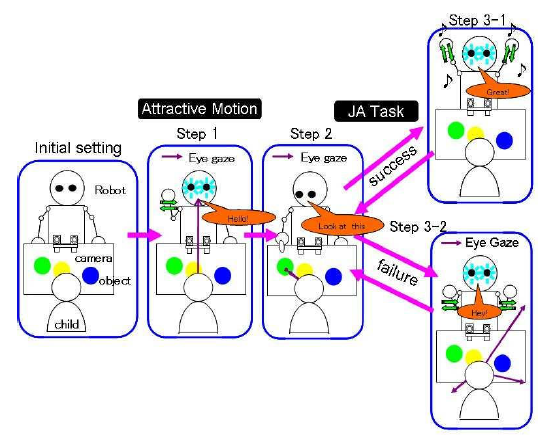
\includegraphics[width=0.6\textwidth]{./img/ravindra2009therapeutic.png}
	\caption{Robot behavior loop used by Ravindra et al. \cite{ravindra2009therapeutic}}
	\label{fig:ravindra2009therapeutic}
\end{figure}

In Diehl et al.'s review, it was pointed out that studies in skill training would benefit from integrating robots into the ABA framework \cite{diehl2012clinical}.  As discussed in Section \ref{sec:DTTDiscussion}, this is what we propose any skill training ATC system should do, similar to COACH.  Thus including a robot into our COACH system would fill this research gap.


In all, from these studies, we see a great potential for increasing the attention and engagement level of the ASD child if we incorporate a humanoid robot into our COACH system.  The robot may serve as an attention grabber as well as a prompting agent.

\section{Visual Focus of Attention Estimation}
%Some kind of intro is needed here on why it is important to review the literature in this area.  It doesn't come across anywhere that this is a key technique you are using and why.
One of the key initiators of communication is joint attention, and grabbing and maintaining the visual attention of the user is an important functionality in the design of socially assistive robots \cite{torta2012can}.  In the context of this thesis, a robot is used to teach and practice hand-washing skills with children with ASD.  In its interaction with the child, successfully grabbing and maintaining the child's attention during the activity will ensure the child receives the prompts as the robot delivers it, and thus increasing the chance that the child complies to the prompts.  To this end, the robot behaviors need to be engaging to the child.  But more importantly, the robot behaviors should be contingent to the child's behaviors.  If the child is not paying attention, for example, an attention grabber (e.g. robot waves hand and call out to the child) would serve as a communication opener before delivering the prompt.  This enables the system to adhere to the DTT prompting framework mentioned in \ref{DTTDiscussion}.  Because of this, the robotic system needs to be able to detect the visual attention of the child in real-time.

\subsection{Visual Focus of Attention and Gaze}
If we define Visual Focus of Attention (VFOA) as what a person is looking at, then given that we know what and where objects of interest are in the scene, the problem for VFOA estimation becomes estimating the direction and depth of a person's visual focus (i.e., gaze).
%Are there not standard definitions of these things that you can use and reference?

For consistency, we define the 3 degrees of freedom (DOFs) of head pose as pan, tilt, and roll (see Figure \ref{fig:murphy2009head}), with reference direction for pan and tilt being frontal direction of the head facing the camera.  We define 2 DOFs of eye pose as pan and tilt similar to head pose, with reference direction for pan and tilt same as head pose.
\begin{figure} [h]
	\centering
	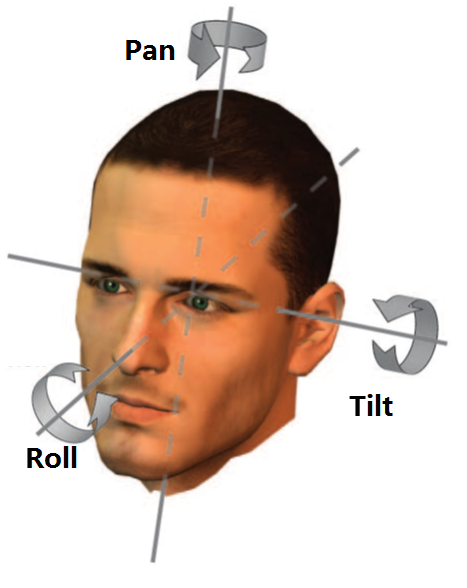
\includegraphics[width=0.6\textwidth]{./img/murphy2009head.png}
	\caption{DOFs of Head Pose, adapted from \cite{murphy2009head}}
	\label{fig:murphy2009head}
\end{figure}


Then, gaze direction is given by the accumulated rotation of average eye pose on head pose \cite{funes2013person}, gaze depth is given by the intersection of the left and right eye pose directions.  Therefore, the problem can be divided into head pose estimation and eye pose estimation.


\subsection{Head Pose Estimation}
There has been extensive research for head pose estimation for a single image frame, or head tracking for a video stream of images.  As reviewed by Murphy-Chutorian et al., the following categories of methods have been identified: appearance templates, detector arrays, nonlinear regression methods, manifold embedding methods, geometric methods, and flexible models \cite{murphy2009head}.


\subsubsection{Appearance Templates and Detector Arrays Methods}
Appearance templates methods and detector arrays methods are mainly for estimating discrete / coarse head pose.  For our task of identifying the object of interest under visual focus of attention, we do not know a priori where and how close to each other the objects are.  Therefore, only continuous fine pose estimation methods are of interest and are reviewed in this thesis.


\subsubsection{Nonlinear Regression Methods}
Using a machine learning approach, a direct mapping from the cropped head image to pose can be learned.  Because such mapping is highly nonlinear, nonlinear regression methods, such as Support Vector Regressors (SVR) \cite{li2000support} and Neural Networks (Multilayer Perceptron (MLP) \cite{voit2008head}, and Locally Linear Map (LLM) \cite{kruger2002gabor} have been applied in this context as supervised learning, using head images as inputs and head poses as ground truths.

Although neural networks are among the most popular and accurate methods in head pose estimation, they are prone to errors from poor head localizations.  And since, in our application, we cannot restrict user to remain in the center of the camera's field of view at all times, we need to either seek out a separate localization method for cropping the head, or seek a head tracker that doesn't have this problem.  Using face detectors for localization is one solution, but it only works for near frontal poses, bottlenecking the head tracker's operating range.


\subsubsection{Manifold Embedding Methods}
Manifold embedding methods learn a projection from high dimensional image space to some low dimensional space.  The methods are unsupervised learning methods that only require head images and not pose ground truth labels.  Promising techniques include: Isometric feature mapping (Isomap) \cite{raytchev2004head}, Locally Linear Embedding (LLE) \cite{roweis2000nonlinear}, and Laplacian Eigenmaps (LE) \cite{belkin2003laplacian}.


However, due to the fact that they ignore pose labels, the projected low dimensional space may not be capturing appearance variations due to head pose alone, but may also include appearance variations due to identity, lighting, etc., making pose prediction inaccurate.  Although there are work around techniques in the manifold embedding methods to tackle the appearance variations due to identity, more systematic ways to deal with it are seen in the following two methods: geometric methods and flexible model methods.


\subsubsection{Geometric Methods}
Geometric methods use person independent facial features (e.g. corners of eyes and mouth, tip of nose, etc.) to predict head pose.  The relative locations of these features are exploited with geometrical assumptions of a person's face such as parallelism, symmetry and proportion \cite{wang2007enhancement}.


A major caveat of these methods is that their accuracy relies on accuracy of features tracking.  For our scenario of a child washing hands at the sink, where a moderate resolution camera captures a mid-range field of view, features are not guaranteed to be tracked with ease.  Thus, it is better to select head pose estimation methods that don't require local features tracking.


\subsubsection{Flexible Model Methods}
Flexible model methods explicitly models the identity as well as pose of a person's face.  Given a representation of the face, flexible models for shape and texture can be constructed using PCA from a face database to represent the directions in which the face most likely (naturally) deforms.  Using this model, a new face image can be fitted through optimizing both an identity parameter and a pose parameter.  This way, pose can be extracted independent of identity.


There are two popular and related flexible model methods: Active Appearance Model (AAM) and 3D Morphable Model (3DMM).  They differ in the following ways:

\paragraph{Face Representation}
Although both models use triangulated mesh representations of the face, AAM uses a 2D representation while 3DMM uses a 3D one.  Also, AAM uses a sparse mesh with vertices at local features while 3DMM uses a dense mesh with vertices at the pixel level.  These make AAM more computationally efficient, but on the other hand 3DMM more robust to low resolution image, partial occlusions, lighting variations, and large head rotations.


\paragraph{Face Fitting}
Because AAM operates in 2D, fitting simultaneously the pose as well as the identity parameters requires us to recover a 3D model of the face using a structure-from-motion algorithm and then use the 3D model's weak perspective projection to constrain 2D fitting \cite{xiao2004real}.  3DMM fitting is less convoluted if using a RGB-D camera (e.g. the Kinect camera).  The pose and identity can be fit simultaneously using a non-rigid iterative closest point algorithm (Optimal Step Non-rigid ICP) \cite{paysan20093d}.

\subsubsection{Kinect Fusion}
Very similar to 3DMM, the Kinect Fusion algorithm developed by Microsoft also can be used to build a 3D head model, and track it's orientation through ICP \cite{newcombe2011kinectfusion}.  The main difference between the two algorithms lies in that 3DMM uses the optimal step non-rigid ICP, which uses a parameterized model of a person's face generated by doing PCA of a face model database.  On the other hand, the head model generation from Kinect Fusion simply rely on building a point cloud of the head, thus its model is not parameterized.  Besides this head model generation step that's different, everything else used in head pose tracking are the same -- rigid ICP alignment.  However, since 3DMM focuses on modeling the face while Kinect Fusion is capable of modeling the whole head, Kinect Fusion may perform better in tracking extreme head poses where the face is largely obstructed.  3DMM, on the other hand, can be tolerant of dynamic expressions on a person's face \cite{amberg2008expression}, while Kinect Fusion may yield poorer tracking when the head model deforms.

\subsection{Eye Pose Estimation}
Eye pose estimation for a single image frame, or gaze tracking for video stream of images, have also been extensively researched.  Here we present results from a recent review by Hansen et al. \cite{hansen2010eye}.  Eye pose estimation methods can be categorized as shape-based, feature-based, and appearance-based:


\subsubsection{Shape-Based Methods}
Shape-based methods are seeking to contour fit the shapes of iris, pupil, eye, etc.  Some examples include: a simple model of ellipse fitting the shape of iris or pupil region, proposed by Valenti et al. \cite{valenti2008accurate}; a complex model of deformable template fitting the eye and pupil shape, proposed by Colombo et al. \cite{colombo1999real}.


\subsubsection{Feature-Based Shape Methods}
Feature-based shape methods seek eye structure localization through identifying a set of distinctive local features.  One can use features directly in the intensity image, with features found for example in limbus, pupil, cornea reflections, eye corners, etc.  An example for this is the neural network method by Reinders et al. \cite{reinders1996locating}.  One can also use features in a filter response of the image, for example seen in the method of A Sirohey et al. \cite{sirohey2001eye}.


Both the shape-based and feature-based methods are inaccurate for moderate resolution mid-range field of view images -- they often require a close up view of an eye.  The problem with large field of view containing not only the eye regions is two fold.  First, lower resolution for the eye regions are available, making the above methods less accurate.  Second, without a proper localization of the eyes, false positives arise.  Methods combining head pose and eye pose estimation is an effective way to combat the false positives in a large field of view as well as dealing with large head poses.  It improves accuracy through the two estimators constraining each other in localizations \cite{valenti2012combining}.  However, a better way, as seen in the head pose tracking section of the literature review, is to use appearance-based methods.


\subsubsection{Appearance-Based Methods}
Another approach to deal with moderate resolution mid-field images is through appearance-based methods.  One can directly model the mapping from eye appearance to eye pose, seen by the neural network method of Baluja et al. \cite{baluja1994non}.  However, direct modeling requires large number of training images, the collection of which is a tedious process.  One way to reduce number of training images needed is through template matching with local linear interpolation.  An example of this is the Adaptive Linear Regression (ALR) method of Lu et al. \cite{lu2011inferring}.


The major caveat with these appearance-based methods, as similarly to head pose estimation, is the inability to separate appearance variations in identity from pose.  One way to tackle this is through keeping a bank of personal models, seen in Mora et al. \cite{funes2013person}.  A new person's eye images can then be represented by a linear combination of exemplar eye images from people in the bank using ALR.  Then, to ease computational cost of ALR, we only keep the top few models that have their exemplar eye images used most often, decreasing the search space during ALR's optimization step.


\subsection{Using RGB-D Camera for Gaze Estimation}
The works of Mora et al. are good fits to our application \cite{funes2012gaze, funes2013person}.  Specifically, their approach uses the 3DMM head pose estimation together with ALR eye pose estimation.  One thing to note is that the commercial grade RGB-D camera, Kinect, is used.  Although 3DMM works with 2D camera as well, getting a direct sensor input on the depth information is advantageous in this context because it avoids inferring the 3D structure from 2D images, reducing inaccuracies and computations. Also, it enables 3DMM to estimate pose through shape alone, ignoring texture fitting altogether, reducing computations and increasing robustness to lighting.


\subsection{Discussion}
From the reviews, we see that Kinect Fusion and ALR are ideal for our application.  They yield many advantages:  Firstly, usage of appearance-based methods means we are moderate resolution mid-field scenario ready.  Secondly, only a simple calibration step is needed to generate the head model for Kinect Fusion and a bank of people's exemplar eye images are needed for ALR.  For the children with ASD population, having relatively simple calibration step that doesn't require the child to behave in a certain way is very useful.  Next, once the person's head model is generated, pose can be fitted without fitting identity, reducing computations.  Lastly, the head image can be restored to the frontal head pose and a consistent frontal eye region cropped out, making eye pose estimation robust to large head poses.



\chapter{Research Objectives}

\section{Overall Goal and Approach}
Our overall goal is to increase a child with ASD's engagement level during COACH prompting and task execution, and thus improving prompt compliance and task completion rate.  Our approach is:
\begin{enumerate}
	\item to incorporate a half body humanoid robot, NAO T14 (see Figure \ref{fig:HalfBodyNAO}) by Aldebaran Robotics, into the current COACH setup, capable of delivering verbal and gesture prompts and attention grabbers.

	\item to automatically track the VFOA of child for more effective maintenance of child's attention.  For example, by being able to recognize whether child is looking at the robot, the robot can call out child's name with a waving gesture or blink its LEDs for getting child's attention before prompting.

\end{enumerate}
\begin{figure} [h]
	\centering
	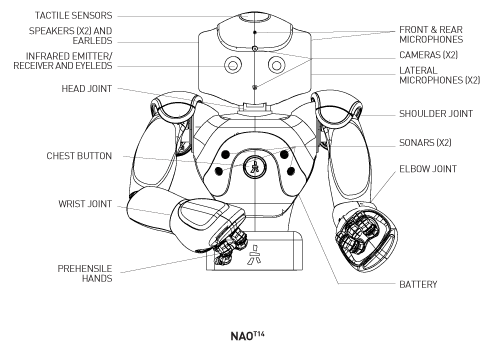
\includegraphics[width=0.6\textwidth]{./img/nao_t14_schema}
	\caption{The Half-Body Version of Humanoid Robot NAO}
	\label{fig:HalfBodyNAO}
\end{figure}


\section{Central Hypothesis}
We hypothesize that the incorporation of a humanoid robot prompting agent, such as NAO T14, would sufficiently capture and maintain children with ASD's attention during prompting and keep them engaged during task execution, so that high prompt compliance rates and task completion rates would be achieved when assisting them through ADLs such as hand-washing.


\section{Specific Objectives}

\paragraph{Our objectives are:}
\begin{enumerate}
	\item To investigate if a prompting system using NAO is able to guide child with ASD through hand-washing.

	\item To explore the different modes of interactions between NAO and child when prompting hand-washing steps using a Wizard of Oz setup, focusing on verbal, gestures, and gaze for the modes of interactions

	\item To implement a real-time algorithm for tracking child's VFOA
\end{enumerate}



\paragraph{Our hypotheses are:}

%	\item Child has greater general engagement level when interacting with NAO than with the parent.


%general engagement level:
%# of times child smiles
%# of times child murmurs
%# of times distracted

%visual focus correct:
%look at prompting agent given prompt rate
%look at step attempted given attempt rate

%prompt compliance and task completion:
%compliance rate
%# of prompts till compliance
%time duration till compliance
%task completion rate
%# of prompts till finished step before prompt
%time duration of extended steps
%number of presses for soap
%# of times requiring physical intervention

%independence:
%# of times child start step before prompt
%# of times child finishes step before prompt

%what measures for survey? just qualitative report? any processing / analysis needed before reporting?

\begin{enumerate}
	\item The humanoid robot, NAO, is able to independently assist child with ASD through hand-washing, and child exhibits greater engagement level, higher prompt compliance rate, and better task completion when prompted by NAO than by parent.

	\item Gestural, gaze, and verbal are the essential modes of interactions present in the hand-washing prompting scenario between child with ASD and the prompting agent NAO.

	\item Using 3DMM and ALR for estimating head pose and eye pose, and using the Kinect camera, a classification rate of more than 80\% is achieved for estimating child's VFOA on NAO, monitor screen, soap, towel, tap region, hands, and idling.

\end{enumerate}

\chapter{The Wizard of Oz Pilot Study}

%What are we trying to find out? Why are they important?
%	- is there a difference in child's response to parent prompt vs robot prompt?
%		- visual attention
%		- compliance
%		- task performance

One major objective of this thesis is to investigate the impacts that using a humanoid prompting agent has on the visual attention, prompt compliance, and task performance of children with ASD during hand-washing activities.

This is the first research of its kind in the field of humanoid robot prompting agent guiding children with ASD through an activity of daily living.  Therefore, it is wise to begin with a pilot study, the purpose of which is to show plausibility of the key underlying assumptions of our hypotheses, and to probe what questions are important to be answered later in a more rigorous randomized control trial.  For this reason, the pilot study should be exploratory in nature, having a flexible experiment design, and relatively low experiment setup cost.

%WoZ experiment design
%	- what is WoZ? why do we use this scheme?
%	- experiment design, why use this design
%	- short blurb of the experiment
%Recruitment
%	- inclusion criteria
%	- method of recruitment, target sample size
%NAO
%	- overall description, capabilities
%	- general design decisions for
%		- verbal prompts
%		- gesture prompts
%Protocol and Setup
%	- experiment / equipment setup for data collection
%	- protocol
%	- video data to be collected
%	- survey to be collected
%	- ethics considerations
%Video annotation protocol
%Measures
%Analysis and results:
%	- participants recruited
%	- video data collected
%	- video analysis method
%	- video analysis results
%	- inter-rater agreement analysis and results
%	- survey data collected
%	- survey analysis method and results
%Discussion:
%	- results interpretations
%	- interpretation limitations
%	- original objectives achieved or not
%	- future outlook

\section{Wizard of Oz Experiment Design}

The Wizard of Oz (WoZ) is an experiment design widely used in Human Computer Interaction (HCI) and Human Robot Interaction (HRI) research.  In a typical WoZ study, there is an interactive agent that is not yet fully autonomous, and is remotely controlled by a human operator (i.e. the "wizard"), and this fact is concealed from the user being tested until after the study.  The wizard may control one or many parts of the agent, such as speech recognition and understanding, affect recognition, dialog management, utterance and gesture generation and so on \cite{bhargava2013demonstration}.  The advantage of a WoZ study is that it does not require a large amount of work spent in implementing the artificial intelligence (AI) behind the agent -- it is taken care of by the wizard.  This is great for testing hypotheses early on in the design loop, enabling us to obtain feedbacks from users, learn, and iterate through design cycles faster.  Of course, care needs to be taken to ensure the mocked up part of the AI is implementable in the near future, since the real purpose of the mock up is to have an early knowledge of the real design constraints, not trying to provide a less constrained solution.

The characteristics of a WoZ study fits our pilot study requirements, where we want to learn early the important design questions regarding building an effective ADL prompting robotic agent for the children with ASD population.  Thus, we conducted a WoZ study, in which a humanoid robot whose motions and speech were preprogrammed, but the decision and timing of their executions were controlled remotely by the researcher.  This is mocking up the computer vision algorithms that understand the child with ASD's actions, the speech recognition algorithms that recognize the child with ASD's verbal interactions, and the AI decision making algorithms that decide what prompts to deliver and when to deliver them.

During each WoZ study trial, the child with ASD would be asked to complete the hand-washing activity in the washroom with the supervision of one of his/her parents, with the help of the NAO robot, or with the help of both the parent and the robot. The researcher, and the parent if the child was to be assisted only by the robot, would be in an adjacent room out of the child's view to observe his/her hand-washing activity.  However, the parent could enter the washroom if the child needed physical assistance to complete a step. A controlling interface running on a laptop, connected wireless to the robot, was used by the researcher to remotely control the robot, as well as to monitor the progress and responses of the child through the video feeds of the cameras installed in the washroom.


\section{Recruitment}

Participants were recruited from a list of families of a previous autism study that indicated that they would be interested in participating in future studies related to the development of the COACH prompting system.

Participants were to be children between the ages of 4 to 15 with a diagnosis of ASD, and their parent. Six children would be recruited. This sample size is typical for studies of this nature for children with ASD. For example, a pilot study by Bimbrahw et al. \cite{bimbrahw2012investigating} and a Wizard of Oz study by Bhargava et al. \cite{bhargava2013demonstration} both involved a similar sample size of the children with ASD in their studies. Another reason we chose six children for this pilot study is to equally explore the two permutations of experimental conditions (i.e. A-B-C and A-C-B, see Section \ref{sec:ProtocolOverview}). Participant demographics would be recorded and would include age, sex, and the Social Responsiveness Scale (SRS) test results.  The SRS is a commonly used tool to identify the presence and estimate the severity of ASD \cite{constantino2002social}. The results of the SRS would allow the research team to substantiate a diagnosis of an ASD for the child participants before proceeding with the study.

\paragraph{The \textbf{inclusion criteria} for enrolling in the study were as follows:}
\begin{itemize}
	\item Boys and girls between the ages of 4-15
	\item Parent report of a clinical diagnosis of an ASD – to be confirmed through administration of the Social Responsiveness Scale (SRS)
	\item Has difficulty independently completing self-care activities, specifically hand-washing
	\item Has the ability to follow simple, one-step verbal instructions
	\item Ethical consent  granted by parents or primary guardian
	\item Does not exhibit severely aggressive behavior
\end{itemize}

Each participating family were given a \$200 honorarium per child subject upon completion of the study. All participants were able to withdraw from the study at any time. The honorarium would then be adjusted to be proportionate to the number of visits completed (e.g. completing 3 visits means the participated child would receive \$100 (\$200 * 3 / 6 = \$100)). This would be made clear to participants at the time of consent.

\section{Humanoid Robot NAO}

We chose the torso and arms only version (T14) of the commercially available humanoid robot NAO from Aldebaran Robotics as our robotic prompting agent.  NAO is a humanoid robot about half a meter high in torso (see Figure \ref{fig:NAOColor}).  It is designed by Aldebaran Robotics to primarily serve academic research in robotics.  NAO is equipped with the state of the art mechanical, electrical, embedded, control, and local network communication systems.  It also has cameras and sonar sensors for computer vision algorithms for scene understanding, path planning, and obstacle avoidance.  The software development kit (SDK) provided is very easy and powerful to program with.  Also, an even easier graphic user interface (GUI) for robot behavior programming, the Choreographe software, is also available.  One caveat of using NAO for SAR HRI researches is that it is only equipped with a single degree of freedom finger dexterity, though other joints in its body are much more mobile.  It is more than enough for doing simple pointing and other non-contact gestural prompts in sync with verbal interactions.  It just cannot perform detailed hand gesturing.  This makes NAO less capable in demonstrating a hand-washing step in high detail.
\begin{figure} [h]
	\centering
	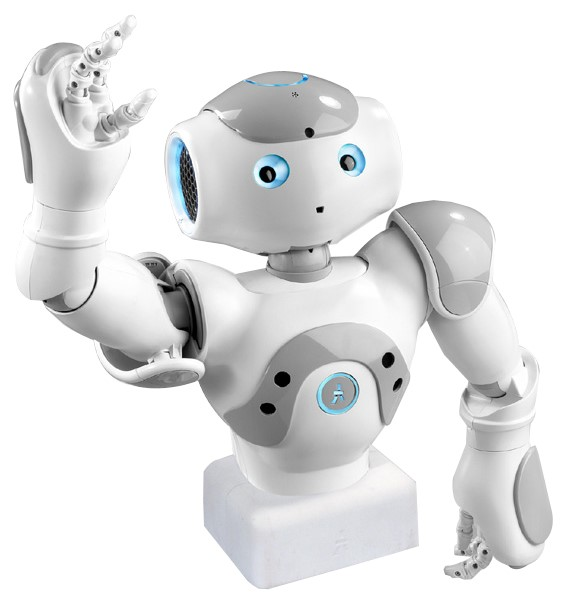
\includegraphics[width=0.6\textwidth]{./img/nao-torso.jpg}
	\caption{NAO T14 Humanoid Torso}
	\label{fig:NAOColor}
\end{figure}


From a HRI research perspective, Aldebaran Robotics took care of designing the intrinsics level of HRI, where NAO has a likable appearance and child like neutral gender voice, although it's incapable of facial expressions.  The design decisions we face when using NAO for this thesis is on the behavior level of HRI.  Design decisions such as voice intonation choice, verbal prompts, motion gestures and gaze, and eye blinks using LEDs in eye regions are made in this thesis.  The objective of this thesis is then to ultimately find out if the lower two levels of design decisions made are able to cumulate to the child with ASD perceiving NAO as a role model / supervisor / assistant during hand-washing.

For our pilot study, we use the half-torso version of NAO because we do not require any mobility from NAO -- it is fixed on the sink table top (see Figure \ref{fig:ExpSetup}).  The relevant functionalities of NAO we utilized for delivering prompts include:
\begin{itemize}
	\item Verbal prompting through its bilateral loud speakers on the head and speech synthesis functionality
	\item Body gesturing through its moving head and arms (although its fingers are not capable of hand gesturing)
	\item Flashing LEDs on the eyes and ears
\end{itemize}
\begin{figure} [h]
	\centering
	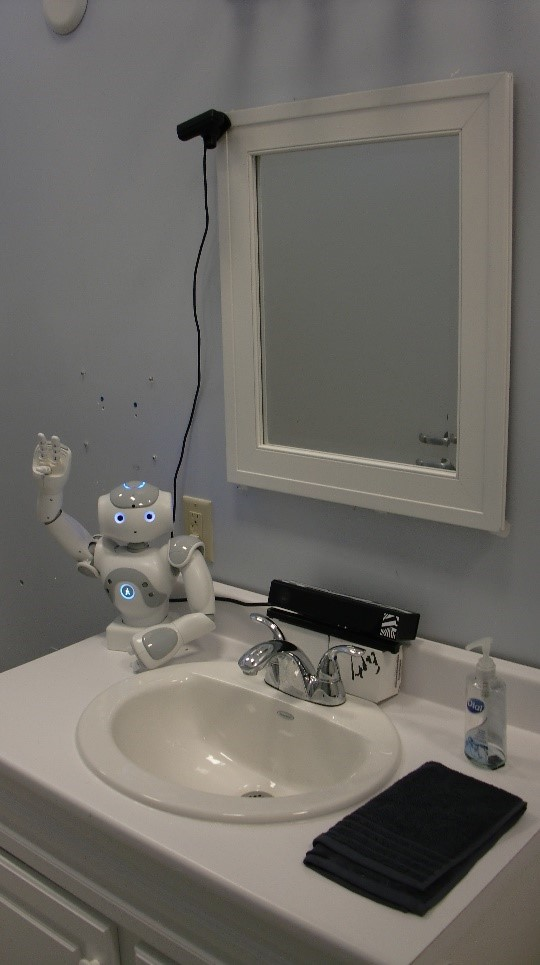
\includegraphics[height=15cm, keepaspectratio]{./img/exp_setup.jpg}
	\caption{Experiment Setup}
	\label{fig:ExpSetup}
\end{figure}


\subsection{Verbal Prompts}
We used the text-to-speech engine from NAO to synthesize the verbal prompts.  The pitch of NAO's voice was changed to a lower one than default for the verbal prompts to give a more authoritative feeling.  The reward verbal prompt remained the default pitch, though, to give an exciting praise.  The verbal prompts were worded as short, three or four word phrases, such as "turn on the water" or "rinse your hand", and a pause is put between the action and the subject so that the prompts sounded clearer and was easier to understand to children with ASD.  The specific choices of verbal and gesture prompts are discussed in Section \ref{sec:SpecificProtocol}.

\subsection{Gesture Prompts}
There are several kinds of gesture prompts NAO needs to perform:

\begin{itemize}
	\item \textbf{Attention grabber (AG)}:  When prompting is needed but the child is not looking at NAO, NAO waves to grab the child’s attention.
	\item \textbf{Motion demonstrating prompt (MoDemo)}:  NAO demonstrates to child the motion of interaction (e.g. turning tap, scrubbing, rinsing, etc.).
	\item \textbf{Object pointing prompt (ObjPt)}:  NAO points to the physical object of interaction.
	\item \textbf{Reward (REW)}:  After a task is successfully completed, NAO flashes LEDs as a positive reinforcement.
\end{itemize}

The gaze behaviour of NAO during gesture prompts is also important and is grouped as: looking at child (when delivering AG, MoDemo, REW), and looking at object (AR, ObjPt).  The gesture and gaze motions can be programmed using NAO's software, Choregraphe.

\subsection{Wizard of Oz Remote Control}
The WoZ experiment setup involves controlling the robot remotely behind the scene by a human operator, the wizard.  A touch screen laptop was used as the user interface for the operator, and the behaviors of the robot were presented as buttons on the screen, with the camera views displayed along side.  Keyboard shortcuts were also implemented for faster access to robot actions.

\section{Surveys}
In addition to observing the child with ASD interacting with the robot, surveys were designed to probe the child's background, experiences, and preferences, putting the observations into context.  Also, surveys probing the parent's opinion of the robot and the COACH system were also created, since the parent is also an important decision maker in the robot and the COACH system's design.

\paragraph{Social Responsiveness Scale Survey and Entrance Survey}
The Social Responsiveness Scale Survey serves to screen participants during recruitment and was filled out by the parent that accompanied the child to all trials.  The entrance survey was administered with the SRS survey, because it reports the child's demographics as well as inclusion criteria fit.  In addition, it also reports child's previous experiences with technologies, child's personal preferences, child's abilities on hand-washing and on other ADLs, and parent's expectation and concerns.

\paragraph{Post-Intervention Survey}
During the last visit, the same parent who completed the SRS survey and the entrance survey was be asked to fill out the post-intervention survey.  The survey reports the parent's opinion on our robot prompting system, giving suggestions and comments and how effectiveness and appropriate is the system, and any improvements or adjustments needed.

\section{Protocol and Setup}


%protocol:
\subsection{Entrance Survey and SRS}
Prior to their first visit to the lab, the parent was asked to complete the Social Responsiveness Scale (SRS). If the child met the SRS score (minimum of 76 T-score), the same parent would then be asked to complete the entrance survey before their first visit. The same parent who has completed the entrance survey was required to accompany the child through all the visits.


\subsection{Protocol Overview}
\label{sec:ProtocolOverview}
The trials were carried out in the washroom inside the HomeLab -- a laboratory specifically designed to emulate the home settings, located on the 12th floor of Toronto Rehab Institute (more details of the experimental environment is described in Section \ref{Sec:ExpSetup}).  Each child would visit the HomeLab once a week with a total of six visits with his/her parent. The six visits would be evenly divided into three phases. The three phases are the baseline phase (Phase A) and the intervention phases (Phase B and Phase C). In Phase A, the child would be asked to wash hands by him/herself as independently as possible. The parent was instructed to provide assistance (as outlined below) to the child as the parent saw necessary.  In Phase B, the child would be assisted by the robot NAO alone.  The parent was out of view in the room adjacent to the washroom, and came into the washroom to prompt when the parent saw necessary.  In Phase C, the child would be assisted by NAO and the parent together.  The parent remained in the washroom and assisted robot NAO in its prompts.

Each visit would take about an hour to an hour and a half. The child was to be asked to wash his/her hands eight times for every visit, for a total of forty-eight trials per child.  This way, the consecutive trials conducted within a day was hopefully not too much for the child to cause fatigue.  Also, having sixteen trials per phase gives a sufficient sample size for both quantitative and qualitative (visual) analyses.  The child and his/her parent could take short breaks after each hand-washing trials.  The break could last as long as the child needed until he/she was willing to continue the trial. If the parent felt the need, they could leave and come back to finish the rest of the day's trials another day. They would not be withdrawn from the study unless requested.

The participating subjects would be randomly assigned one of the two phase orders: A-B-C and A-C-B.  This would reduce the confounding effect of learning when we compare between phase B and C.

\subsection{Experiment Setup}
\label{Sec:ExpSetup}
The equipment was set up near the sink, which includes a NAO robot, an overhead camera, a scene camera, and a Kinect camera. The NAO robot is a small half-torso humanoid robot and was screw-mounted on the sink countertop at the top left corner (please see Figure \ref{fig:ExpSetup}). The NAO robot delivered verbal and gesture prompts to the children with ASD while they were performing the hand-washing tasks.  The overhead camera was installed on the wall/mirror right above the sink. The overhead camera recorded objects on the sink countertop (e.g., taps, faucet, soap, and towel). The purpose of the overhead camera is to capture the hand actions of the child during hand-washing in order to track the child’s progress along the tasks. The scene camera was placed on the floor with its field of view including all objects in the scene (e.g., robot, child, and objects on sink countertop). The purpose of the scene camera is to capture the child’s engagement and attention during the prompts as well as during task executions. The Kinect camera was mounted on the sink countertop underneath the mirror and behind the tap. The Kinect camera recorded mainly the child’s face. The purpose of the Kinect camera is to capture the child’s face during hand-washing for the development of an automatic algorithm that estimates the child’s gaze direction in real-time. Examples of the images captured by the three cameras are shown in Figure \ref{fig:CameraViews}.
\begin{figure}[H]
	\centering
	\begin{subfigure}[b]{0.49\textwidth}
		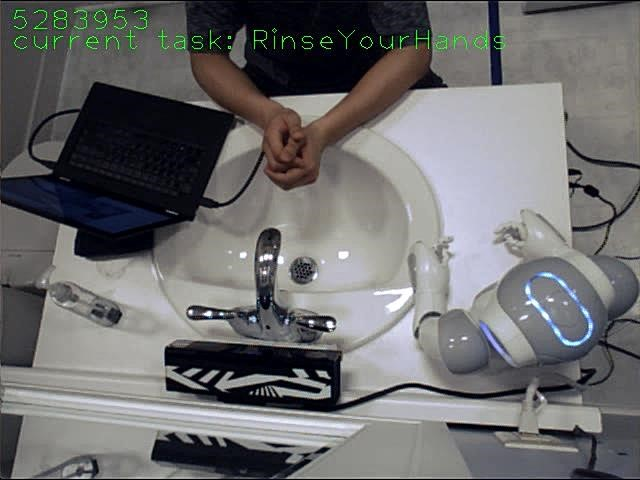
\includegraphics[width=1.1\linewidth]{./img/overhead_view.jpg}
		\caption{Overhead Camera View}
%		\label{fig:7TotalNumberofIncompleteSteps-BeforeParentorRobotPrompts}
	\end{subfigure}

	
	\begin{subfigure}[b]{0.49\textwidth}
		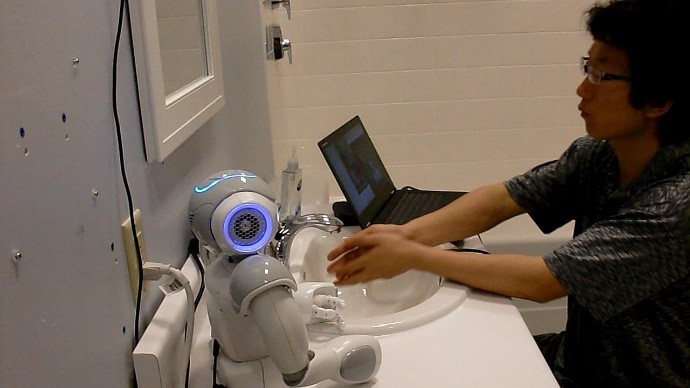
\includegraphics[width=1.1\linewidth]{./img/scene_view.jpg}
		\caption{Scene Camera View}
%		\label{fig:6TotalNumberofIncompleteSteps-BeforeParentPrompts}
	\end{subfigure}%

	
	\begin{subfigure}[b]{0.49\textwidth}
		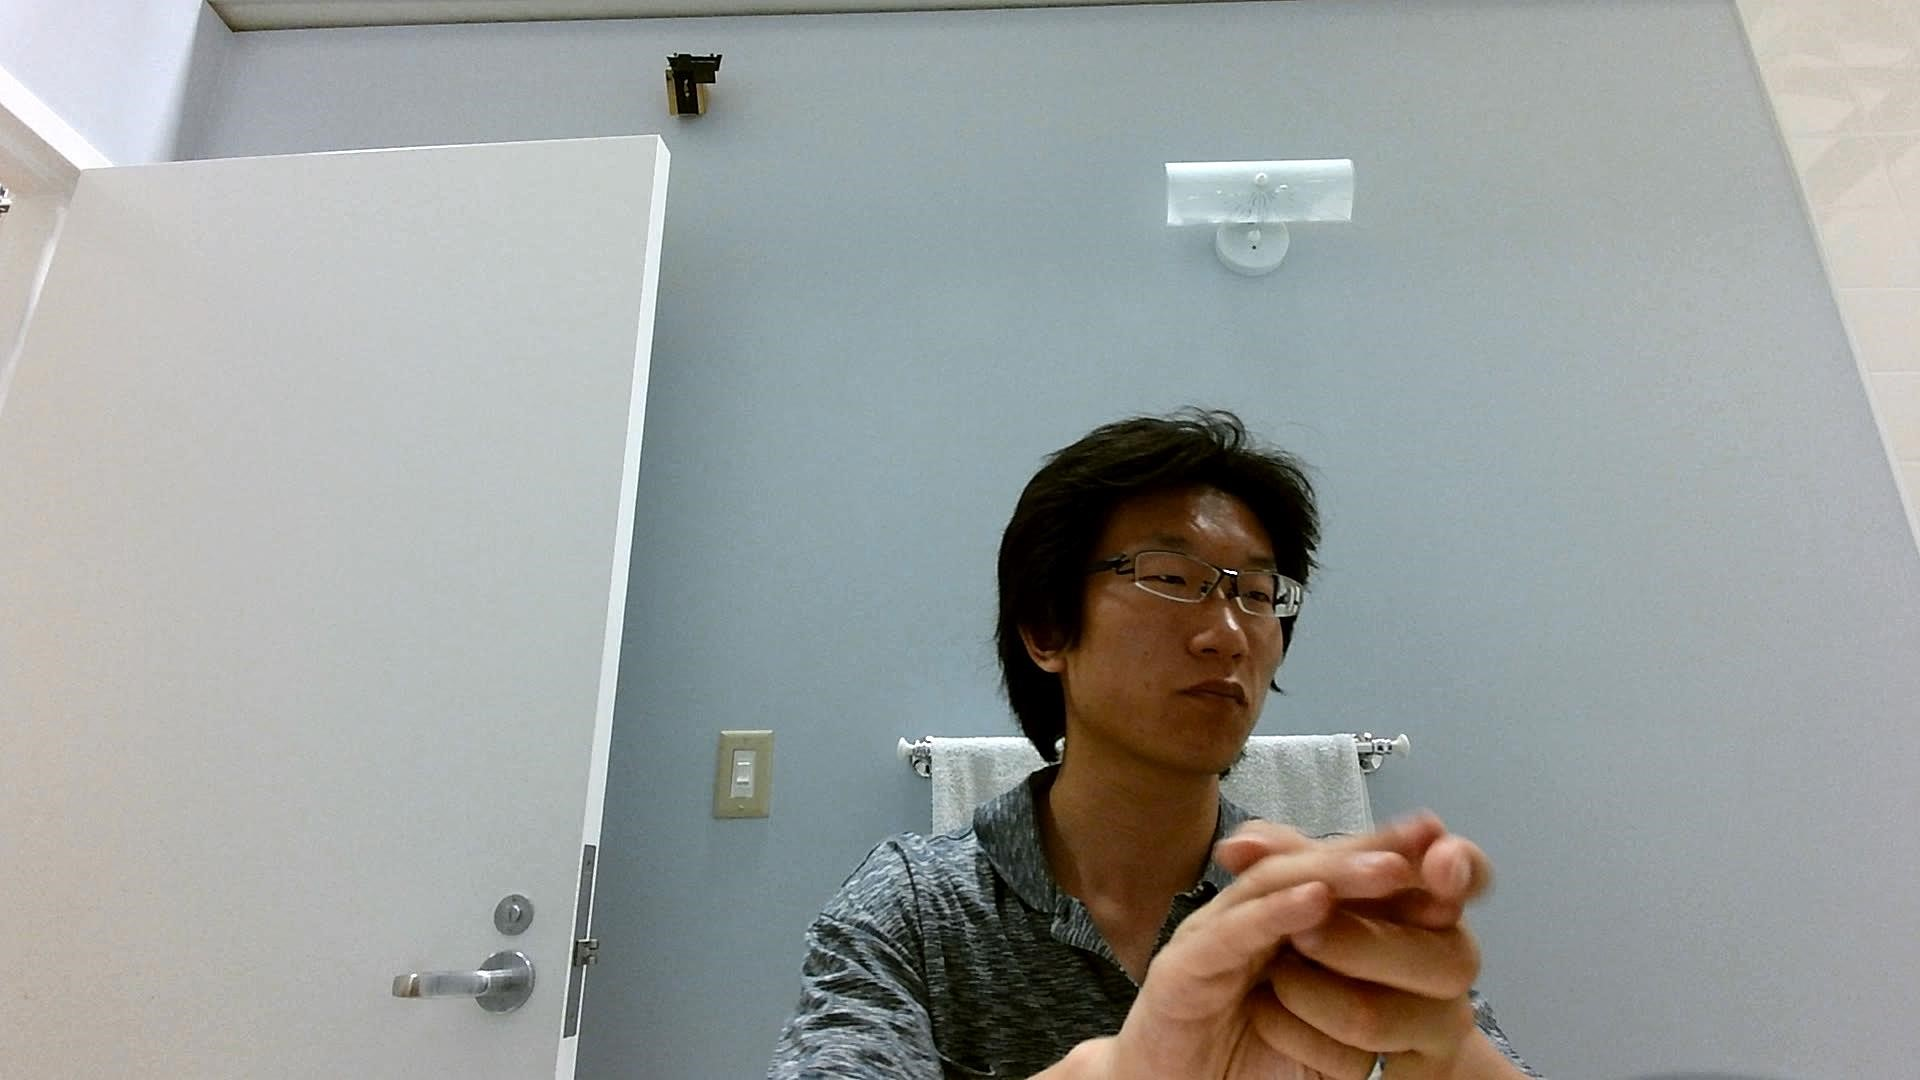
\includegraphics[width=1.1\linewidth]{./img/kinect_view}
		\caption{Kinect Camera View}
%		\label{fig:5TotalNumberofIncompleteSteps-BeforePhyiscalPrompts}
	\end{subfigure}%

	\caption{The views of the three cameras used in the WoZ study.}
	\label{fig:CameraViews}
\end{figure}


A touchscreen laptop was used during the study by the student researcher to control the robot and the virtual avatar displayed on the LCD screen. It connects to the robot wirelessly. The laptop also connects to the overhead and Kinect cameras through USB cables to provide real-time video feed. The data collected from the cameras was saved temporarily in the laptop hard-drive. 

\subsection{Specific Protocol}
\label{sec:SpecificProtocol}
The hand-washing activity was broken down into seven steps: turn on the water, wet your hands, get some soap, scrub your hands, rinse your hands, turn off the water, and dry your hands.  These steps were a modified version based on Bimbrahw et al. pilot study \cite{bimbrahw2012investigating}. These constitute the same steps as Bimbrahw's except that the first (i.e. turn on the water and wet your hands) and the last step (i.e. turn off the water and dry your hands) are now four individual steps to ensure that each step only involves one action.

\paragraph{Phase A (Baseline Phase)}
The first phase was the baseline phase and would include sixteen trials of hand washing. The child would be asked to complete the hand-washing as independently as possible. During this phase, the parent would be present in the washroom while the child was completing the hand-washing steps. The parent would verbally and/or physically assist and give positive reinforcements to the child whenever the parent feels necessary.

\paragraph{Phases B and C (Intervention Phases)}
The rest of the two phases were the intervention phases and would include sixteen trials of hand washing each. The child would be asked to wash his/her hands with the help of NAO or of both NAO and the parent in the washroom. During each trial, NAO and the parent would wait for the child to start each step. If the child experienced troubles, an appropriate prompt would be delivered from NAO in order to help the child complete the step. If the child did not respond to NAO's prompt, an attention grabber would be delivered to capture the child's attention to the prompting agent. The attention grabber could be repeated for a second time if the child failed to respond to the first one.  A verbal reward would be delivered to the child when he/she completed a step.

The parent's role in phase B and C differs in that, in phase C, the parent would take a more active role to prompt the child of what to do by standing next to the child.  On the other hand, in phase B, the parent would take more of a back seat role, being out of view and coming in to prompt only for the purpose of reminding the child to listen to the robot, but leaving the prompting of the specific step to the robot.  Of course, if the child didn't respond to any of the prompts, the parent would need to physically intervene and complete the step together, just like in phase A.  After the physical intervention, the parent would then instruct and encourage the child to continue the rest of the hand-washing steps on his/her own by following the robot.  Both phase B and C are important.  Phase B serves to test if NAO can independently assist the child through hand-washing with minimal parent involvement.  Phase C serves to investigate whether and why would NAO be more effective in assisting the child when parent is present.  Comparing phase B and C would potentially yield areas of improvement for NAO.

There are three prompt categories that the NAO robot would deliver when interacting with the child (please see Table \ref{tab:RobotPrompts} for the specifics of each prompt used):
\begin{enumerate}
	\item \textbf{Step Prompt} (to prompt the child through a hand-washing step):

	A verbal prompt is delivered, such as “Please [step name]” (e.g. “Please turn on the water.”).  Synchronous to the verbal, a visual prompt is also be delivered. This is a two-part gesture prompt of: first, demonstrating the motion of interaction while looking at the child (MoDemo); second, pointing to the sink object (e.g. the tap) while looking at the object (ObjPt). A maximum of two prompts is given to the child. If the child does not respond to the second prompt or has started the step but does not complete the step within the a reasonable time, the parent is asked to help the child complete the step. 

	\item \textbf{Attention Grabber} (to catch the child's attention to the NAO robot): 

	A verbal prompt is delivered, such as “Hi, [child's name]!”  Synchronous to the verbal, a visual prompt is also delivered. This is an attention grabbing gesture of waving and looking at the child (AG). A maximum of two attention grabbers is given to the child in order to get his/her attention to look at the robot.  The parent is asked to instruct the child to look at the robot if he/she does not respond to the second attention grabber. 

	\item \textbf{Reward} (to provide positive reinforcement when the child attempts a step without the help from his/her parent): 

	A verbal reward (i.e. “Great!”) is delivered while looking at the child and switching back and forth the colors of the light-emitting diodes (LEDs) on the eyes after successfully performing a step (REW).
\end{enumerate}
\begin{table}[h]
	\centering
	\begin{tabular}{ |l| p{4cm} | p{8cm} | }
		\hline
			&	\textbf{Verbal Prompt}	&	\textbf{Robot Gestures}	\\	\hline

		\textbf{Attention Grabber}	&	Hi, [child's name]!	&	Waving and looking at the child.	\\	\hline

		\multirow{7}{*}{\textbf{Task Prompts}}	&	Turn on the water!	&	Turning right wrist clockwise while looking at the child, then pointing and looking at the tap.	\\	\cline{2-3}
		&	Wet your hands.	&	Holding out hands while looking at the child, then pointing and looking at the running water.	\\	\cline{2-3}
		&	Get some soap.	&	Pressing down right hand with left hand collecting from below while looking at the child, then pointing and looking at the soap.	\\	\cline{2-3}
		&	Scrub your hands.	&	Scrubbing both hands while looking at the child, then pointing and looking at the child’s hands.	\\	\cline{2-3}
		&	Rinse your hands.	&	Holding out hands while looking at the child, then pointing and looking at the running water.	\\	\cline{2-3}
		&	Turn off the water.	&	Turning right wrist counterclockwise while looking at the child, then pointing and looking at the tap.	\\	\cline{2-3}
		&	Dry your hands.	&	Wiping one hand against the other while looking at the child, then pointing and looking at the towel.	\\	\hline

		\textbf{Reward}	&	Great!	&	No gestures. Flashing multicolor LEDs on the eyes while looking at the child.	\\	\hline

		\textbf{Intro}	&	Hi, [child’s name]! Let’s start washing hands.	&	Giving an attention grabber gesture followed by a simple conversational gesture while looking at the child.	\\	\hline

		\textbf{Re-intro}	&	Let’s continue washing hands.	&	Giving a simple conversational gesture while looking at the child.	\\	\hline

		\textbf{Outro}	&	Good job, [child’s name]! You are all done.	&	Fist pumping in the air, followed by an all done gesture. Flashing multicolor LEDs on the eyes while looking at the child.	\\	\hline
	\end{tabular}
\caption{The Robot Prompts -- Detailed Descriptions.}
\label{tab:RobotPrompts}
\end{table}

For each trial, in addition to the three prompt categories stated above, the NAO robot would also deliver a short introduction before the start of each trial, a re-intro after the parent finished assisting the child through a step, and an outro at the end of each trial. The introduction is a two-part prompt. The first part is an attention grabber. The second part consists of a verbal prompt (i.e. “Let's start washing hands.”) with a simple conversational gesture. The re-intro is a verbal prompt (i.e. “Let's continue washing hands.”) with a simple conversational gesture. Same as the introduction, the outro is a two-part prompt. The first part consists of a verbal prompt (i.e. “Good job, [child's name]!”) with a gesture of fist pumping in the air. The second part consists of a verbal prompt (i.e. “You are all done.”) with a gesture signifying all the hand-washing steps have been done.

\subsection{Post-intervention Survey}
During the last visit, the same parent who completed the entrance survey would be asked to fill out the post-intervention survey.

\subsection{Data Collection}
All phases were video recorded by the overhead, the scene, and the Kinect cameras and audio recorded by the microphone from the scene camera.  The overhead and scene video data would be reviewed and annotated by an annotators. The overhead video data would be used to score the participants' prompt compliance and hand-washing performance. The scene video data would be used to evaluate the participants' engagement during the whole activity. The effectiveness of robot prompting on engagement, compliance, and performance would then be explored qualitatively and quantitatively.

The Kinect video data would not be annotated. Instead, it would be used to evaluate the automatic gaze estimation algorithm that we developed. Specifically, the Kinect video data would be used by the gaze estimation algorithm as input and the output predictions would be compared with annotations of the scene video data to derive the algorithm's prediction accuracy.



\subsection{Ethics}
The WoZ was approved by the Research Ethics Board (REB) of University Health Network (UHN), belonging to which is the Toronto Rehab Hospital, where the study was conducted.

\paragraph{Consent and Assent}
Participants were given a package of consent/assent forms prior to starting the study. One of the parents would need to provide their consent for their child and themselves to participate in the study. In addition, child participants would need to provide their assent to participate in their every visit of the study. 

Interested families would receive an information/consent package prior to starting of the study. This package includes consent/assent forms for participation in the study for the parent and child with ASD (these forms include study details and research contact information) as well as consent to be videotaped for the parent and child with ASD. Consent from the parent and assent from the child with ASD would be given if and when they feel comfortable that they understand the information presented. Potential participants of both parents and children had up to a week to decide if they would like to participate, although they may consent to participate as soon as they feel comfortable doing so. Parents would need to provide their consent for their children and themselves to participate in the study. In addition, child participants would need to provide their assent in their every visit of the HomeLab during the study to participate. Parents would be required to consent to having their children and themselves videotaped during the study. The parents would be informed that they and their children may withdraw from the study at any time without penalty.

\paragraph{Confidentiality}
Each participating family (parent and child with ASD pair) would be assigned a code number when they sign the consent/assent. All data in the study would be labelled with these code numbers only - the names of the participants would appear only on the information and consent/assent forms and would be kept confidential. Consent forms would be placed in a secure and locked area in the PI's laboratory, with access exclusively restricted to the research team. All forms will be destroyed seven years after the study publication. 

The information and data collected would remain strictly confidential and would not affect any of the participants (both the parent and the child)' employment, care, or treatment in any way. A code number would be assigned to each parent and child participant when they give consent. This code number, instead of their name, were used for all data collection and analysis. Direct quotes may be included in the final research paper but names would not be used in any report or publication. Privacy of participants (both the parents and the children) were ensured by omitting all participant information from participant data, by employing data encryption, and by storing data on a secure server.  If and only if participants consent, participants (both the parents and the children) video data could be presented for educational purposes.  If any images or videos were used in presentations and publications, faces and other identifiable features would be masked.

Both the video and audio data would be stored temporarily on the touchscreen laptop's hard drive during each child's visit. The data would be encrypted and transferred to the TRI servers as soon as after each child's visit. The portable devices, such as USB sticks, would be used to transfer the data to the TRI servers. All files stored in the portable devices would be password protected and encrypted. The data on the laptop's hard drive and the portable devices would then be purged immediately after transfer. 

\paragraph{Data Storage}
All soft (electronic) data would be encrypted before any transfer is made. All data would be password protected and be stored on the TRI servers with access restricted to the research team. The laptop used for the study were password protected so that only the research team has the access to it. All computerized data would be password protected. All survey data would be stored in a locked cabinet different from where the consent forms are stored. Access to all the data would be restricted only to the supervisor and researchers involved in the project. 

After the study is completed and the results of the study are published, data will be stored for at least seven years from study closure. All data will be destroyed seven years after the study closure. Data contained on paper material will be destroyed by shredding the material. Data contained on electronic media will be destroyed by erasing or other removing the data in such a way that it cannot be retrieved. 


\section{Measures}
\label{sec:measures}

\subsection{Video Data Measures}
To evaluate the effectiveness of the robot prompts on child's step completion, to measure the child's compliance to the prompts, and to investigate their relationships with the child's engagement level during hand-washing, the following metrics are calculated and analyzed from the video data annotations for each trial:


\paragraph{Prompt Effectiveness}
\begin{itemize}
	\item \textbf{Total Number of Complete Steps}: the number of hand-washing steps that were completed.
	\item \textbf{Total Number of Parent Prompts}: the number of prompts delivered by the parent (e.g. verbal, pointing, motion demonstrations, nudging, guiding, and physically intervening).
\end{itemize}

\paragraph{Responses to Prompts}
\begin{itemize}
	\item \textbf{Compliance Rate}: the percentage of prompts that the child followed correctly.
	\item \textbf{Not Affected By Prompt Rate}: the percentage of prompts that the child ignored.
\end{itemize}

\paragraph{Engagement and Visual Attention}
\begin{itemize}
	\item \textbf{Total Number of Times Child Smiles}: the number of prompt sections that the child smiled.
	\item \textbf{Total Number of Times Child Murmurs}: the number of prompt sections that the child murmured.
	\item \textbf{Looking at Prompting Agent Rate}: the percentage of prompt sections that the child looked at parent when parent was prompting or at robot when robot was prompting.
\end{itemize}

\paragraph{} %a blank space
The specific definitions for each measure will be discussed further in the analysis section \ref{sec:VideoDataAnalysisAndResults}.  The difference between prompts and prompt sections is discussed in \ref{sec:AnnotationFramework}.
\section{Video Annotations}
In order to calculate the final measures outlined above, intermediate measures need to be extracted from the video data.  This is the process of video annotation.
%To compare between P and R in terms of:
%	- visual attention
%	- prompt compliance rate
%	- step completion rate
%	- starts step before prompt
%	- stops step before prompt
%	- duration of execution

%tables:
%	- annotation keys:
%		- prompting steps, prompting agent, P gesture prompt types
%	- annotation items divided by 3 segments:

%- explain the annotation items in a workflow manner, as if guiding a person through how to annotate a video
%- talk about the tools needed for annotation, the format of the document, and how to annotate in different scenarios

\subsection{Annotation Framework}
\label{sec:AnnotationFramework}
Only the scene camera videos were annotated, since this view alone suffices in informing both the progress of the child in hand-washing steps and the child's response to prompts.

Each video file usually contains one hand-washing trial, sometimes two.  The annotator needs to scroll through each video until the scene of the child entering the washroom, marking it as the start of a trial.  The child leaving the washroom marks the end of a trial.

A trial contains many hand-washing steps, and for each step, the parent and/or the robot may give several prompts.  For consistency and convenience, the annotator divides the video into segments we call ''prompt sections'', and describe each prompt section using a 3-part scheme.  The first part describes the child's actions before any prompts, the second describes the prompting agent's prompts, and the third describes the child's actions after the prompts.  The intermediate measures to be annotated in each part of the prompt section are shown in Table \ref{tab:IntermediateMeasures}.

\begin{table}[H]
	\centering
	\begin{tabular}{ | p{5cm} | l | p{7cm} | }
		\hline
		\textbf{Intermediate Measure}	&	\textbf{Type}	&	\textbf{Description}	\\	\hline	\hline

		Step	&	Nominal	&	Prompting step, 0 no step, 1 intro, 2 turn on water, 3 get soap, 4 scrub hands, 5 rinse hands, 6 turn off water, 7 dry hands, 8 all done, 9 wet hands	\\	\hline \hline

		\multicolumn{3}{|c|}{\textbf{Child's Action Before Prompts}} \\	\hline

		Time Start	&	Ordinal	&	Time stamp for start of prompting section	\\	\hline
		Time Stop	&	Ordinal	&	Time stamp for end of prompting section	\\	\hline
		Attempted Step Before Prompt	&	Nominal	&		\\	\hline
		Attempted Step Successfully Executed Before Prompt	&	Ordinal	&	0 incomplete, 1 complete but low quality, 2 complete with high quality	\\	\hline	\hline

		\multicolumn{3}{|c|}{\textbf{Prompting Agent's Prompts}} \\	\hline

		P Verbal	&	Ordinal	&	Parent verbal prompt, 0 no verbal prompts, 1 prompt for compliance to robot, 2 prompt for step	\\	\hline
		P Gesture	&	Ordinal	&	Parent gestural prompt, 0 no gesture prompts, 1 quick point, 2 sustained point, 3 motion demonstration, 4 motion demonstration and point, 5 nudge, 6 guide arm, 7 do step fully	\\	\hline
		P Reward	&	Boolean	&	Does parent give reward	\\	\hline
		R Verbal	&	Ordinal	&	Robot verbal prompt, same coding as P Verbal	\\	\hline
		R Gesture	&	Ordinal	&	Robot gestural prompt, same coding as P Gesture	\\	\hline
		R Attention Grabber	&	Boolean	&	Does robot give attention grabber	\\	\hline
		R Reward	&	Boolean	&	Does robot give reward	\\	\hline	\hline

		\multicolumn{3}{|c|}{\textbf{Child's Action after Prompts}} \\	\hline

		C Looks At P/R	&	Nominal	&	Child looks at the prompting agent, 0 no looks, 1 looks at parent, 2 looks at robot, 3 looks at both	\\	\hline
		C Smiles	&	Boolean	&	Does child smile	\\	\hline
		C Murmurs	&	Boolean	&	Does child make a verbal sound	\\	\hline

		Attempted Step After Prompt	&	Nominal	&	\\	\hline
		Attempted Step Successfully Executed After Prompt	&	Ordinal	&	Same coding as Attempted Step Successfully Executed Before Prompt	\\	\hline
		Attempted Step Is Correct Although Different From Prompt	&	Boolean	&	Is this one of those times that the prompts are wrong or ambiguous and child's actions make sense despite different	\\	\hline
		Number of Prompts Till C Executes Correct Step - Parent	&	Cardinal	&	Count number of prompts as any distinct actions performed by the parent before child executes the correct step.	\\	\hline
		Number of Prompts Till C Executes Correct Step - Robot	&	Cardinal	&	Same as above, but counting robot prompts	\\	\hline

	\end{tabular}
	\caption{The Intermediate Measures Annotated From the Video Data}
	\label{tab:IntermediateMeasures}
\end{table}

A hand-washing step could have multiple prompt sections.  Take for example the following scenario: The child executes the wrong step before prompts, so the parent prompts the correct step, but the child ignores the prompt and continues the wrong step.  This constitutes one prompt section.  Then the parent prompts again, and the child finally follows the prompt and executes the correct step.  This constitutes then another prompt section.  For this example, because the parent prompts a second time without waiting for the child to stop his/her current action, the second prompt section should have a blank for the Child's Action Before Prompts.

A hand-washing step could also have multiple prompt sections because of the step's nature.  For the ``extended steps'' (i.e. scrubbing, wetting, rinsing, and drying), even when the child is executing the correct step, the prompting agent may deliver more prompts to encourage the child to keep doing the same step for an extended period of time.  This is in contrast to the non-extended steps (e.g. turning on the water), where a single action from the child marks the completion of that step.  An example of an extended step with multiple prompt sections is: The child starts rinsing before prompt, then the parent tells the child to keep rinsing.  The child continues to rinse.  The parent says again ``keep rinsing'', and the child rinses more and then decides to stop.  This constitutes one prompt section.  Then, the parent prompts to rinse more again.  The child follows.  After a while, the parent decides this is enough and prompts for the next step.  This marks the end of the second prompt section.  For the first prompt section, it contains two prompts from the parent.  This is intentional, for the purpose of convenience -- we group any consecutive prompts (can be from either the parent, the robot, or from both) resulting in the same actions from the child as one prompt section.  This grouping does not affect any of our measures for Prompt Effectiveness or Responses to Prompts, since those measures count the number of steps or prompts, not prompt sections.  However, this grouping does affect the measures in Engagement and Visual Attention, since these measures count the number of prompt sections instead.

%Lastly, getting soap is a step similar to the extended steps such that it itself takes an extended period of time to execute.  However, it is different because of the child's tendency to always get more soap than needed.  So after the child starts getting soap, any prompts given are to tell the child to stop the step (as opposed to prolonging the step, as in the other extended steps' cases).  This means the measure, ``child stops step before next prompt'', is marked true if and only if no prompts are given after the child starts getting soap.  In general, ``child stops step before next prompt'' is marked true if the child stops the step before any prompt is given that is either telling him/her to stop (e.g. a verbal reward) or to go on to the next step.

\subsection{Annotation Tools}
The videos are played back by the software Media Player Classic - Home Cinema (MPC-HC 64-bit v1.7.8), where timestamps of millisecond resolution can be obtained.  The annotations are recorded onto Microsoft Office Excel spreadsheets, and each sheet exported to CSV files to be analyzed.

%\subsection{Annotators and Inter-rater Agreement}
%- number of annotators
%- percentage of overlap
%- inter-rater agreement calculation (method, what's good enough)

\section{Data Analysis and Results}


\subsection{Participants Recruited}
Due to limitation of time, we were only able to recruit one subject.  Our participant is a thirteen years old male child of Asian ethnicity.  He was accompanied to the trials by his mother, who was the one that answered all surveys.

\subsubsection{Child's Demographics and Inclusion Criteria Fit}
The child has been clinically diagnosed of Autism Spectrum Disorder.  We also conducted the Social Responsiveness Scale Survey, and he obtained a T-score of 79, passing the minimum score for severe ASD.  Through the Entrance Survey, we learned that the child has difficulty independently completing self-care activities (a 2 on a scale of 1 (not independent at all) to 5 (completely independent)), and this includes hand-washing (also a 2 on the same scale).  We also learned that the child is able to do but not good at verbal communication (a 3 on a scale of 1 (very not well) to 5 (very well)).  Specifically, the child can only speak one or two words at a time to express what he wants, uses iPad for communication, and often just murmurs illegibly.  However, the child has the ability to follow simple, one-step verbal instructions (a 4 on a scale of 1 (very not well) to 5 (very well)).  Lastly, the child does not exhibit severely aggressive behavior (a 1 from a scale of 1 (never) to 5 (often)).  The above shows that the child fits in our inclusion criteria.


\subsection{Experiment Design Change}
We were not able to counterbalance the confounding effect of learning through randomly assigning participants to phase orders (A-B-C versus A-C-B), since we only recruited one participant.  Instead, we decided to control it by splitting the Phase B into two segments, one before Phase C and one after.  Thus, we conducted the study in the following phase order: A-B-C-B (i.e. parent alone phase - robot alone phase - robot parent phase - 2nd robot alone phase).  This way, we can compare first Phase B and second Phase B to see how much does learning in Phase C affect our results.  Also, first Phase B and second Phase B won't have sixteen trials each due to limitation of time.  Instead, we conducted these two phases only long enough to see a stable response, as is typically done in a single-subject research design \cite{ayres2009acquisition, bereznak2012video}.  As a result, we had 16 trials for Phase A, 8 trials for first Phase B, 21 trials for Phase C, and 5 trials for second Phase B.  Note that the intervention conditions of first Phase B and second Phase B are meant to be the same.


\subsection{Video Data Analysis and Results}
\label{sec:VideoDataAnalysisAndResults}

\subsubsection{Analysis Method}
The analyses employed here are visual analyses.  The analyses mainly compare the levels (eyeballing the mean) of measures in different phases.  In cases where the level of a measure changes dramatically within a phase, this trend with initial level and final level were noted.

\subsubsection{Prompt Effectiveness}
To reflect how effective our prompting system is, we show whether the system can reduce both the number of incomplete steps and the number of parent prompts.

\paragraph{Number of Incomplete Steps}
We assumed that parent prompts had a higher level of authority over the child than robot prompts, because the robot only delivered verbal prompts and gestures such as pointing and motion demonstrations, while the parent could deliver those as well as nudging, guiding the arm, and completely executing the step for the child if the verbal and gesture prompts did not work.  This means we can measure the effect of robot prompts by comparing number of complete steps without prompts vs. with robot prompts alone, and measure the effect of parent prompts by comparing number of complete steps with robot prompts alone vs. with robot and parent prompts.  Figure \ref{fig:TotalNumberOfCompleteSteps} shows a series of plots for the measure ``Total Number of Complete Steps'', differing in what steps counted as completed when plotting the figures, e.g. Plot \ref{fig:7TotalNumberofCompleteSteps-WithoutPrompts} (``Without Prompts'') counts only steps completed by child with no prompts from the robot or the parent.  The next Plot \ref{fig:6TotalNumberofCompleteSteps-WithRobotPrompts} (``With Robot Prompts Only''), allows steps prompted by the robot to also count towards completed steps, and Plot \ref{fig:4TotalNumberofCompleteSteps-WithRobotAndParentPrompts} (``With Robot and Parent Prompts'') counts every completed steps even if they were prompted by the parent or the robot.

The most important comparison is between Plot \ref{fig:7TotalNumberofCompleteSteps-WithoutPrompts} (``Without Prompts'') and Plot \ref{fig:6TotalNumberofCompleteSteps-WithRobotPrompts} (``With Robot Prompts Only''), demonstrating the effectiveness of the robot's presence.  We see that parent alone phase (Phase A) was unaffected since robot wasn't present, but introducing the robot in the rest of the phases show effectiveness: robot alone phase (first Phase B) from 2.5 to 3, robot parent phase (Phase C) from 2 to 3, and robot alone repeat phase (second Phase B) from 2.5 to 4.

Comparing Plot \ref{fig:6TotalNumberofCompleteSteps-WithRobotPrompts} (``With Robot Prompts Only'') against Plot \ref{fig:4TotalNumberofCompleteSteps-WithRobotAndParentPrompts} (``With Robot and Parent Prompts''), we see the effectiveness of parent prompts: parent alone phase moved from 3 to 6, robot alone phase from 3 to 3.5, robot parent phase from 3 to 5, robot alone repeat phase from 4 to 4.5.
\begin{figure}[h]
	\centering
	\begin{subfigure}[b]{0.49\textwidth}
		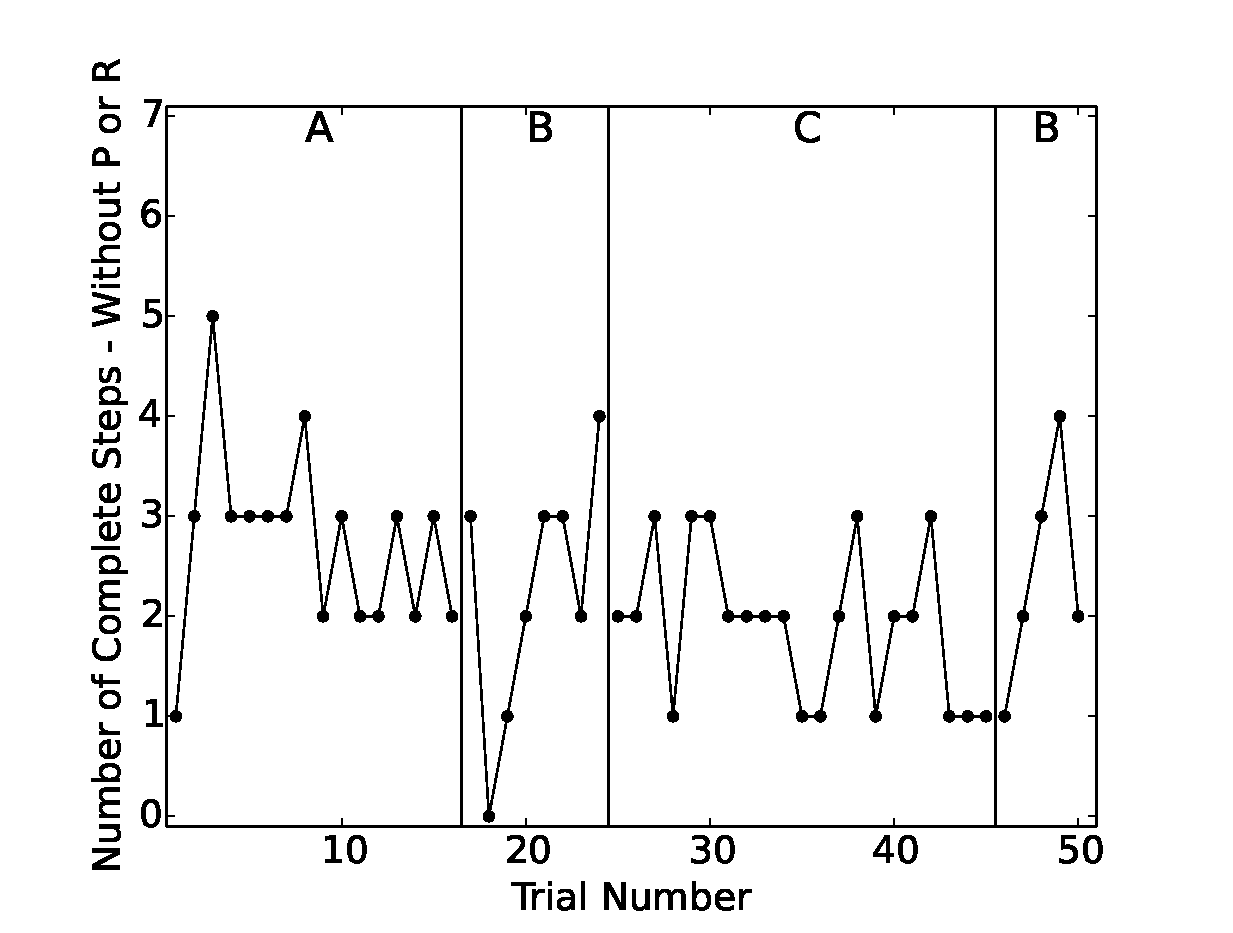
\includegraphics[width=1.1\linewidth]{./img/data_analysis/110NumberofCompleteSteps-WithoutPorR.eps}
		\caption{Total Number of Complete Steps - Without Prompts}
		\label{fig:7TotalNumberofCompleteSteps-WithoutPrompts}
	\end{subfigure}
	\hfill
	%	~ %add desired spacing between images, e. g. ~, \quad, \qquad, \hfill, or double enter etc.	
	\begin{subfigure}[b]{0.49\textwidth}
		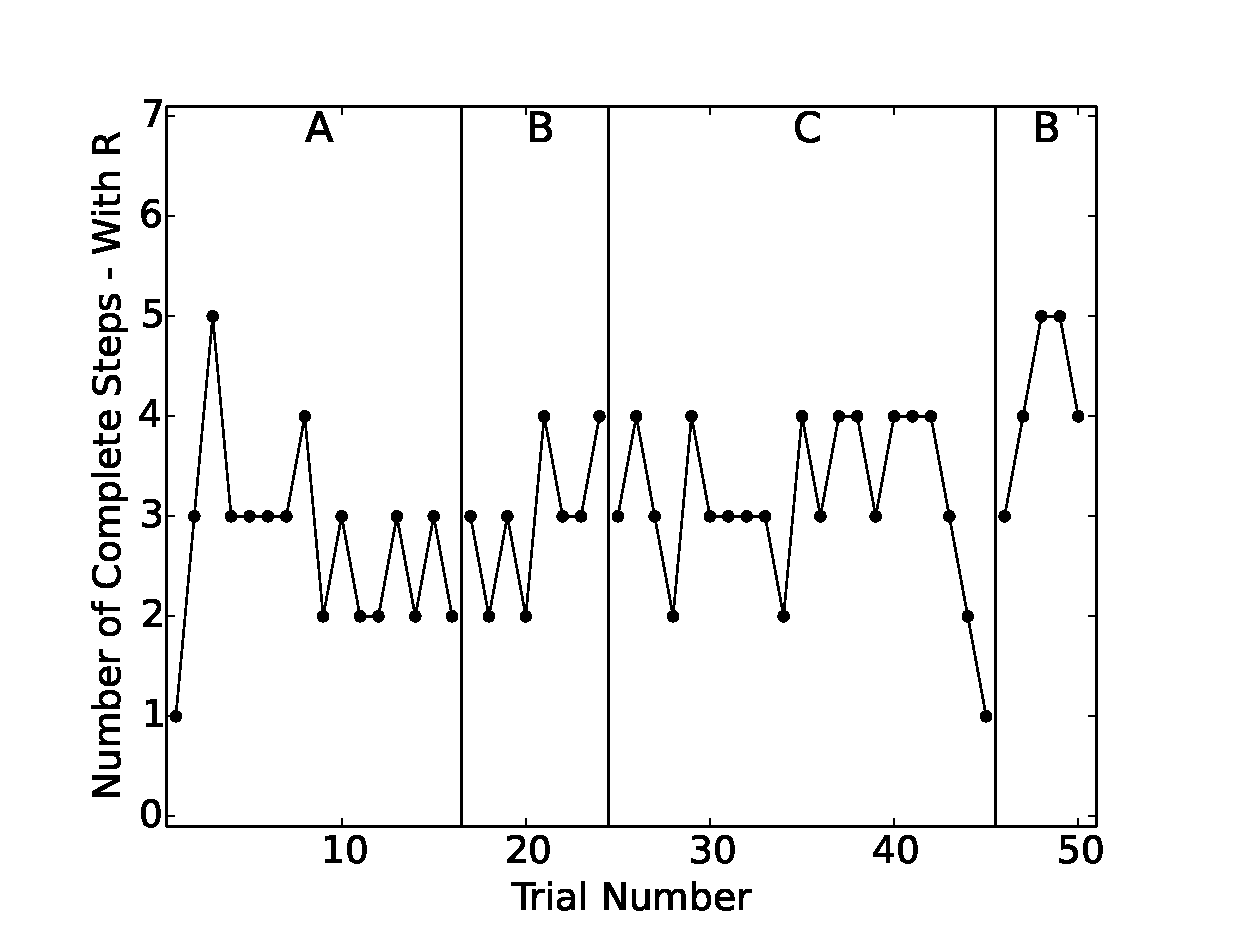
\includegraphics[width=1.1\linewidth]{./img/data_analysis/109NumberofCompleteSteps-WithR.eps}
		\caption{Total Number of Complete Steps - With Robot Prompts Only}
		\label{fig:6TotalNumberofCompleteSteps-WithRobotPrompts}
	\end{subfigure}%

	
	\begin{subfigure}[b]{0.49\textwidth}
		
\includegraphics[width=1.1\linewidth]{./img/data_analysis/blank.png}
	\end{subfigure}%
	\hfill
	\begin{subfigure}[b]{0.49\textwidth}
		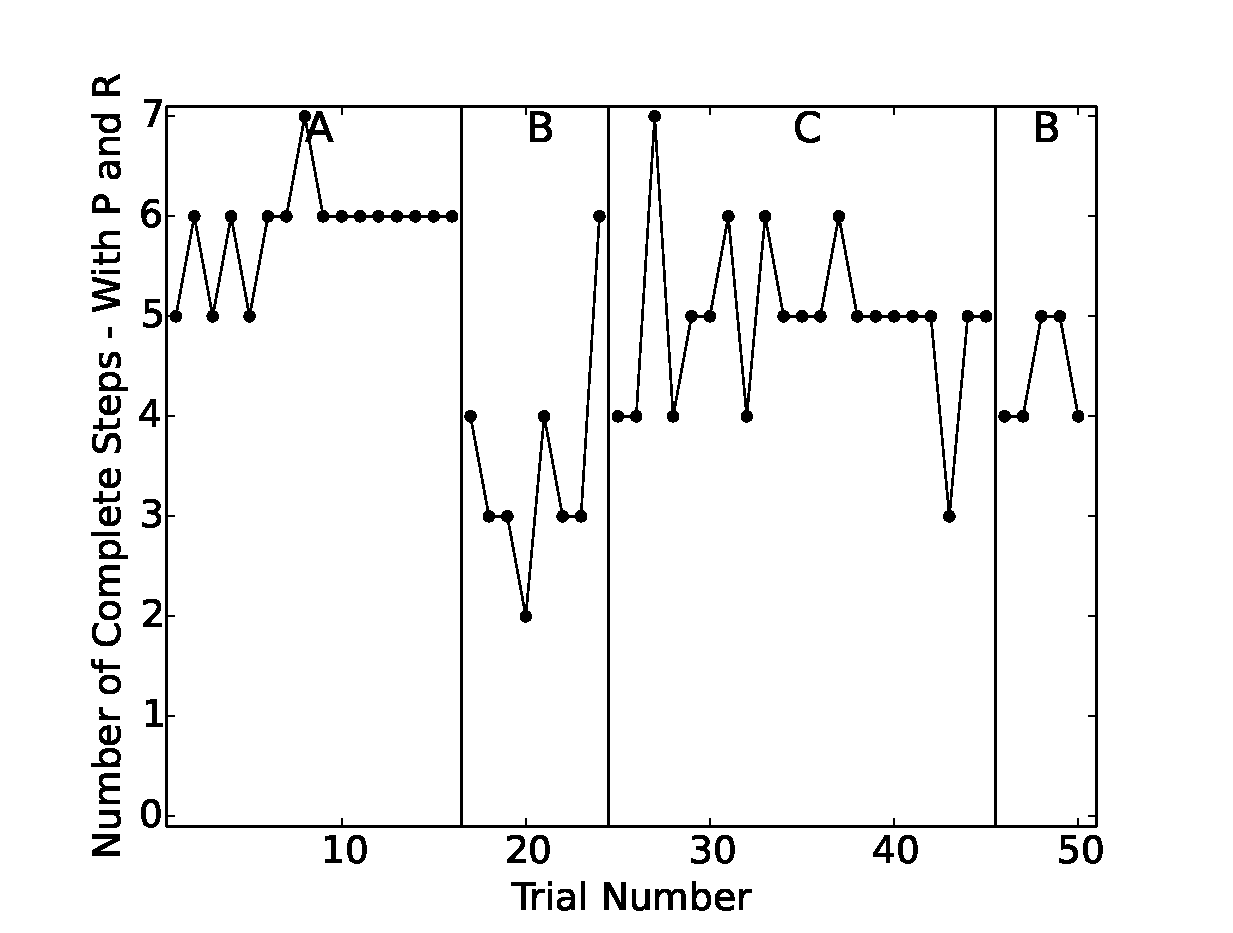
\includegraphics[width=1.1\linewidth]{./img/data_analysis/108NumberofCompleteSteps-WithPandR.eps}
		\caption{Total Number of Complete Steps - With Robot and Parent Prompts}
		\label{fig:4TotalNumberofCompleteSteps-WithRobotAndParentPrompts}
	\end{subfigure}%
	\caption{Total Number of Complete Steps}
	\label{fig:TotalNumberOfIncompleteSteps}
\end{figure}

\paragraph{Number of Parent Prompts}
The measure ``Total Number of Parent Prompts'' is plotted in Figure \ref{fig:TotalNumberOfParentPrompts}.  Plot \ref{fig:25TotalNumberofParentPrompts} is for the overall count (i.e. counting both physical and non-physical prompts).  It shows that during parent alone phase (A), the measure has an upward trend from 5 moving to 20.  However, in robot alone phase (first Phase B), we have a sudden drop leveling at near zero.  In robot parent phase (C), the measure has a downward trend moving from 15 to 5.  In robot alone repeat phase (second Phase B), we again observe a near zero level.  By comparing the measures across phases, we see that the robot's presence were effective in reducing the number of parent prompts, especially in robot alone and repeat phases.  Plot \ref{fig:26TotalNumberofParentPrompts-Physical} is for the physical prompt count.  This plot shows when the parent resorts to a higher prompt level (i.e. physical prompts such as nudging, guiding, and physically intervene) in order to get the child's compliance.  We see that the level is mainly near zero for all phases except for robot parent phase (C), leveling around 2.5.
\begin{figure}[h]
	\centering
	\begin{subfigure}[b]{0.49\textwidth}
		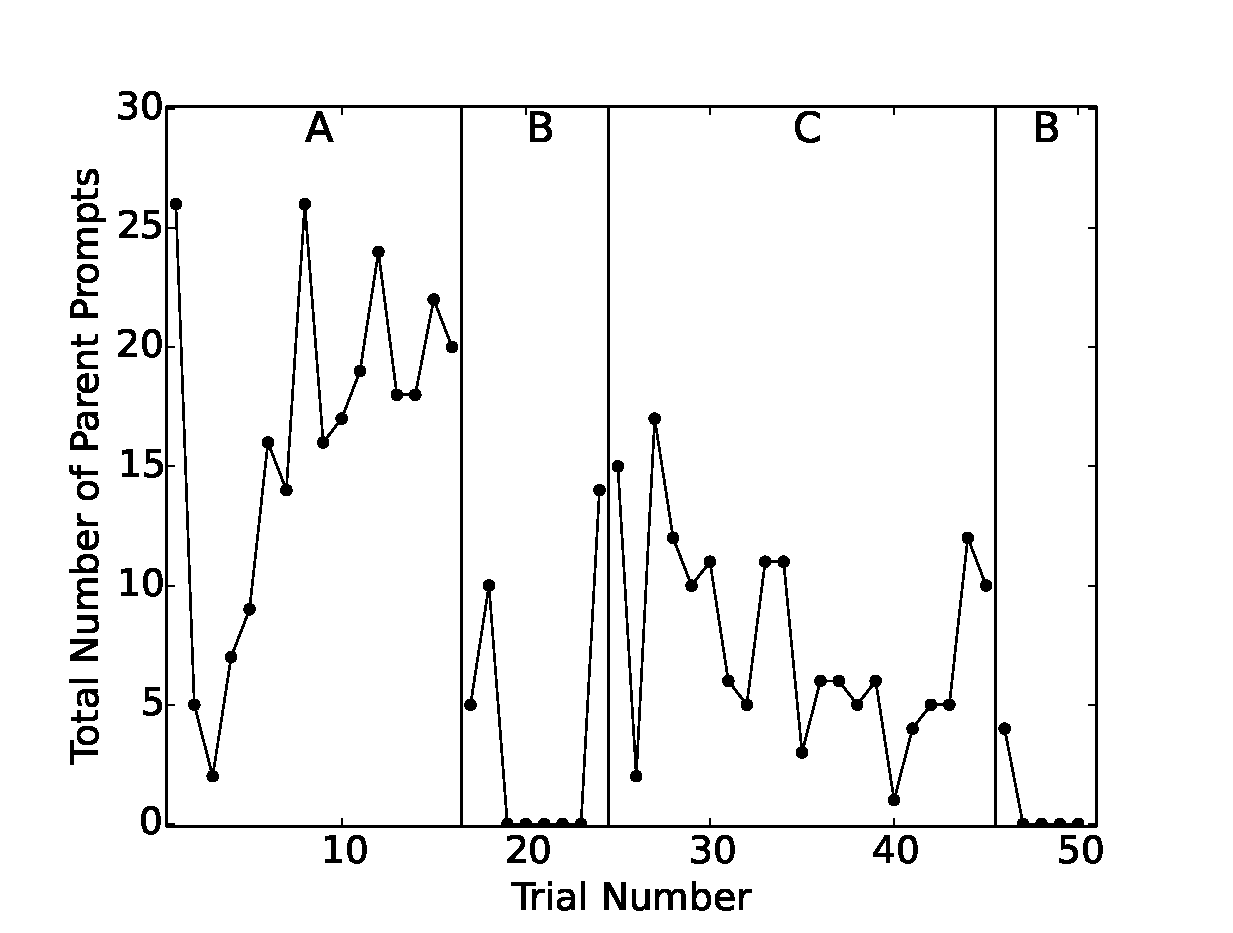
\includegraphics[width=1.1\linewidth]{./img/data_analysis/25TotalNumberofParentPrompts.eps}
		\caption{Total Number of Parent Prompts - Overall}
		\label{fig:25TotalNumberofParentPrompts}
	\end{subfigure}
	\hfill
	\begin{subfigure}[b]{0.49\textwidth}
		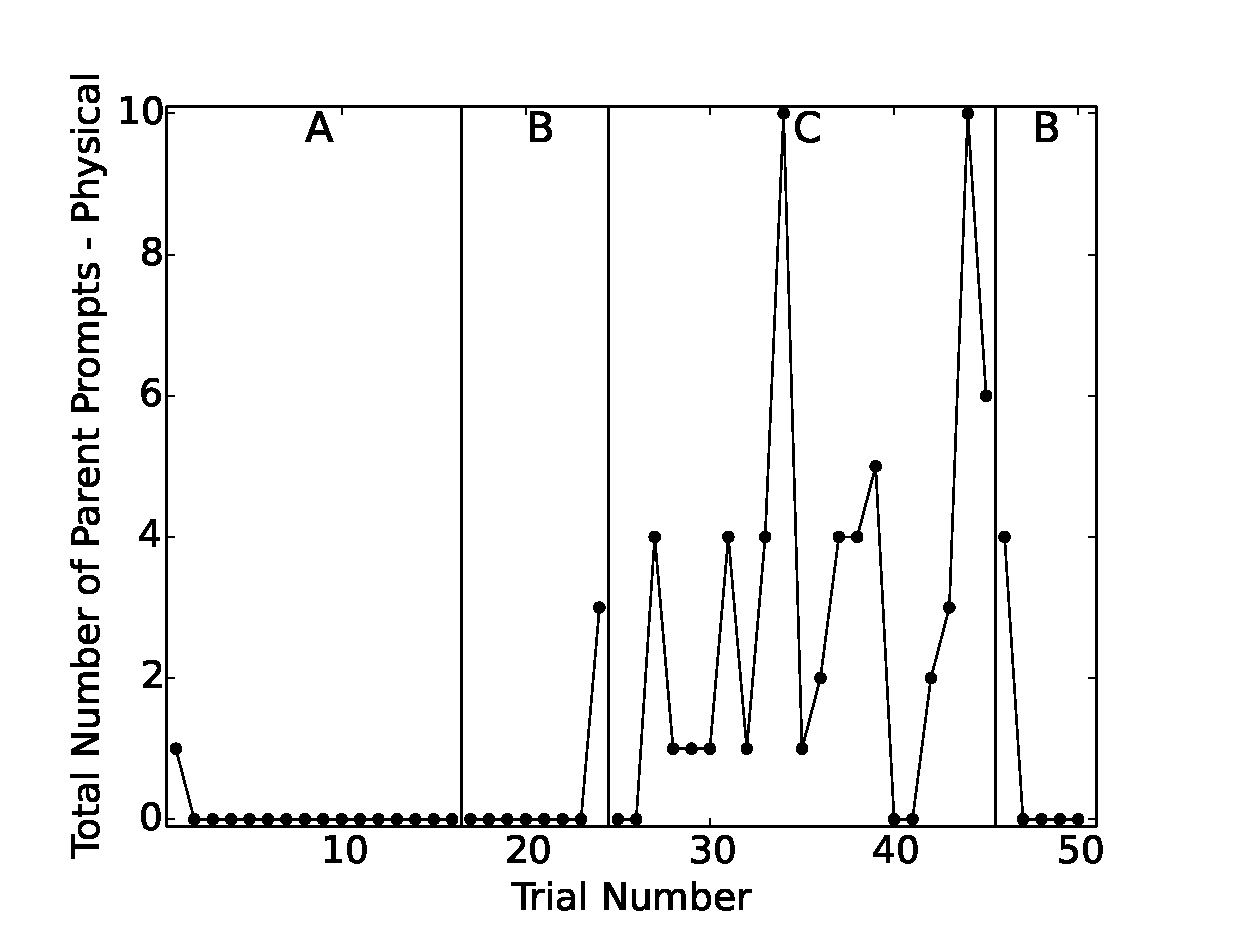
\includegraphics[width=1.1\linewidth]{./img/data_analysis/26TotalNumberofParentPrompts-Physical.eps}
		\caption{Total Number of Parent Prompts - Physical}
		\label{fig:26TotalNumberofParentPrompts-Physical}
	\end{subfigure}%
	\caption{Total Number of Parent Prompts}
	\label{fig:TotalNumberOfParentPrompts}
\end{figure}


\subsubsection{Child's Response to Prompts}
To illustrate the child's different responses to the prompts, we characterized child's responses into three categories: ``compliance'', ``not affected by prompt'', and others.

\paragraph{Compliance Rate}
A response is counted towards ``compliance'' if the child executes the correct step in response to the prompt.  If the child was executing the wrong step before prompt, and is converted into doing the correct step due to prompt, we call this hard compliance.  The compliance and hard compliance response rates are shown in Figure \ref{fig:ComplianceRate}.

Plot \ref{fig:102ComplianceRate-Overall} shows the overall compliance rate, with parent alone phase (A) leveling at 80\%, robot alone phase (first Phase B) leveling at 30\%, parent robot phase (C) moving upward from 60\% to 80\%, and robot alone repeat phase (second Phase B) leveling at 80\%.  We see that when the robot was first introduced in robot alone phase (first Phase B), the child did not comply to the prompts.  However, by going through Phase C where the parent prompts for child to follow the robot, the child complies more readily in the robot alone repeat phase, achieving similar level of compliance as the parent alone phase.  We need to note that this plot includes prompts delivered by the robot, by the parent, and by them together.  Even in robot alone and repeat phases, the parent still comes into the washroom and prompts when the child isn't complying to the robot.  To see whether the robot alone can potentially guide the child through the whole hand-washing activity with minimal parent involvement, we plotted the compliance rate counted over only prompts delivered by the robot, shown in Plot \ref{fig:79ComplianceRate-R1Pv0g0}.  This plot confirms the levels observed in the overall plot, validating the improvement of compliance rate seen in R Alone Rep phase.  To investigate to what extent the child is compliant, the overall hard compliance rate is shown in Plot \ref{fig:103HardComplianceRate-Overall}, with parent alone phase (A) split leveling at 100\% and 35\%, robot alone phase (first Phase B) leveling at 25\%.  The robot parent phase (C) averaging around 60\% but the spread increases as trials went on.  Lastly, the robot alone repeat phase (second Phase B) levels at 50\%.  Similar to above, we observe an improvement of hard compliance between robot alone and repeat phases.  Looking at the robot prompts only Plot \ref{fig:92HardComplianceRate-R1Pv0g0}, the robot alone phase (first Phase B) drops to almost 0\%, while robot alone repeat phase (second Phase B) remains at 50\%.
\begin{figure}[h]
	\centering
	\begin{subfigure}[b]{0.49\textwidth}
		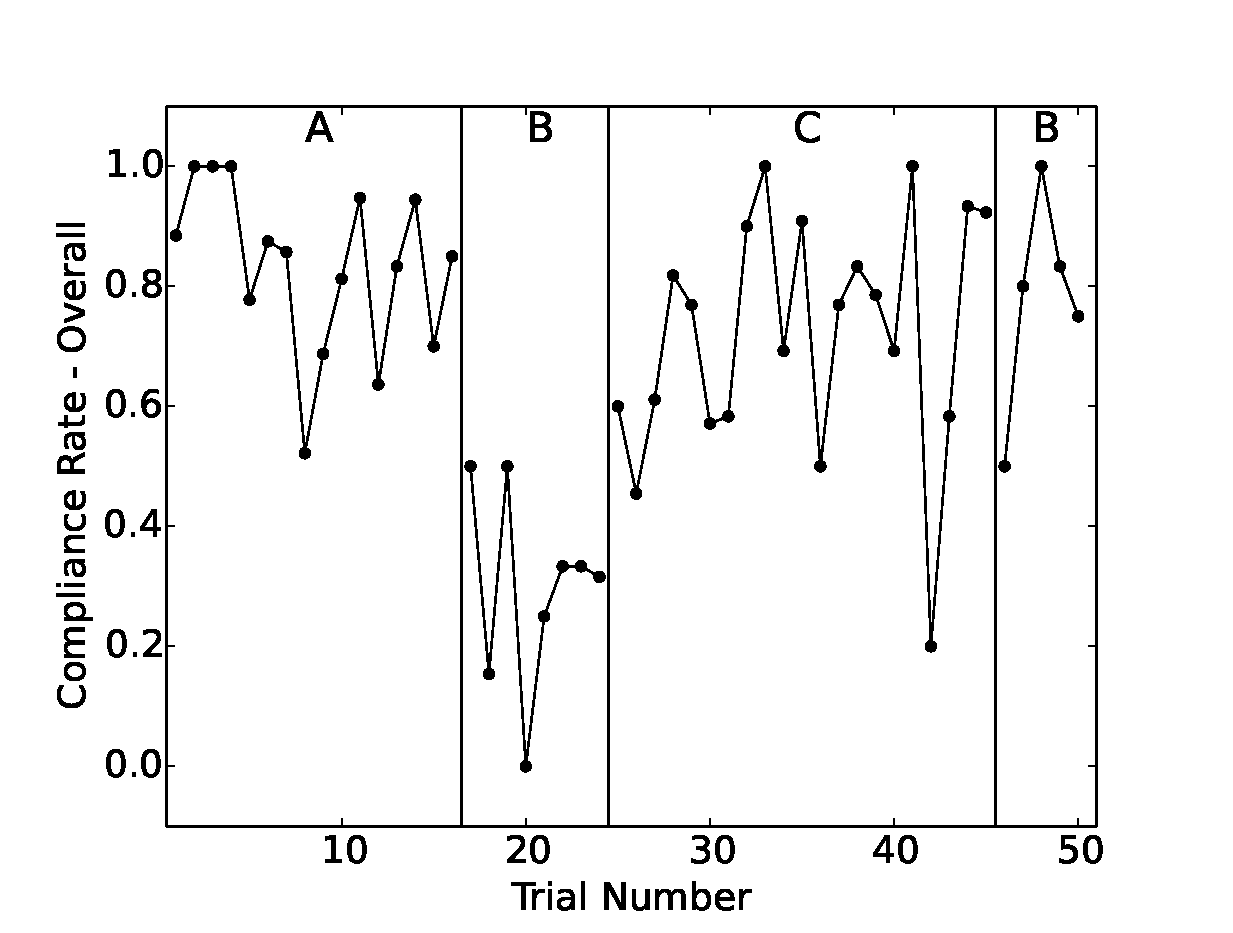
\includegraphics[width=1.1\linewidth]{./img/data_analysis/102ComplianceRate-Overall.eps}
		\caption{Compliance Rate - Overall}
		\label{fig:102ComplianceRate-Overall}
	\end{subfigure}
	\hfill
	\begin{subfigure}[b]{0.49\textwidth}
		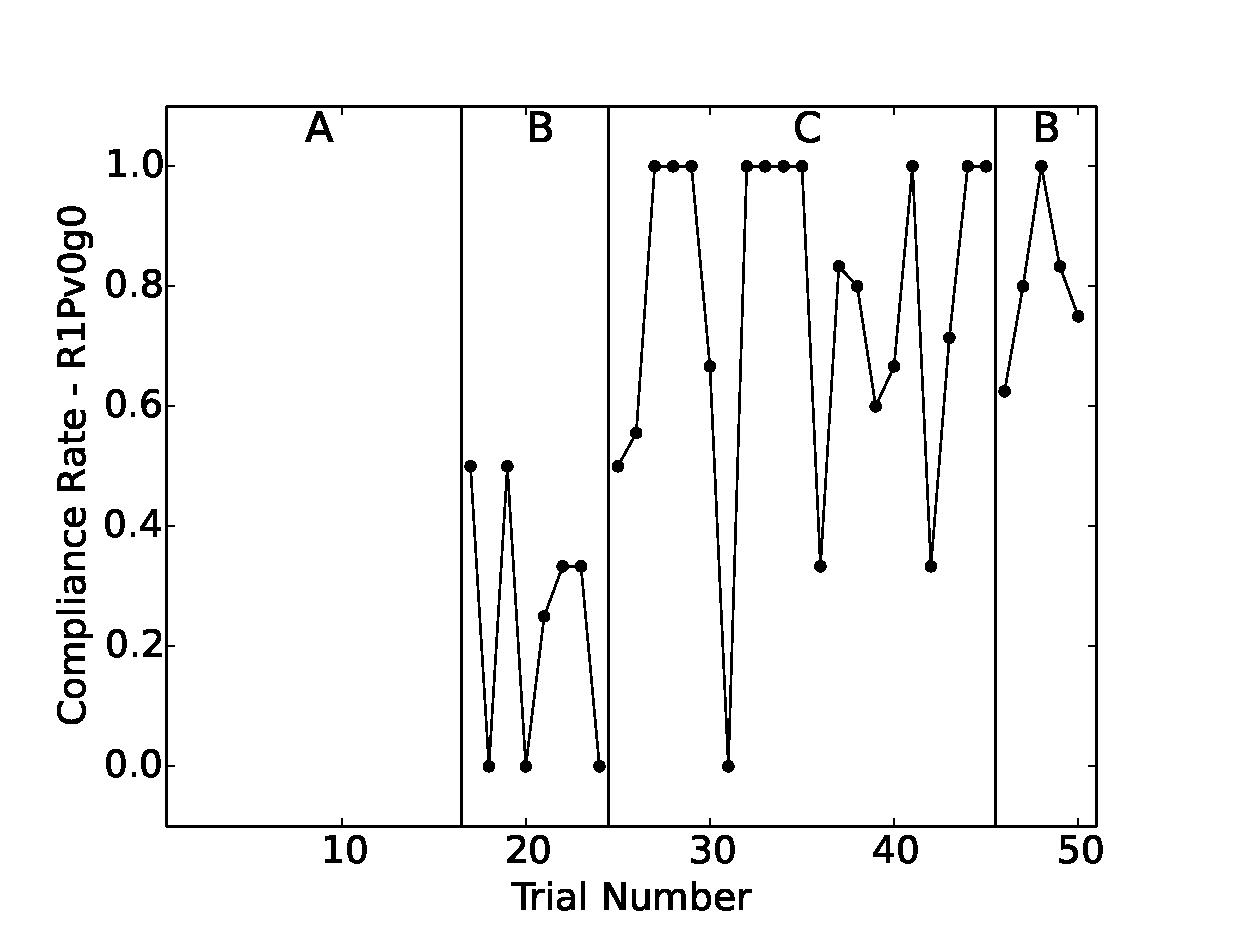
\includegraphics[width=1.1\linewidth]{./img/data_analysis/79ComplianceRate-R1Pv0g0.eps}
		\caption{Compliance Rate - Robot Only Prompts}
		\label{fig:79ComplianceRate-R1Pv0g0}
	\end{subfigure}%

	
	\begin{subfigure}[b]{0.49\textwidth}
		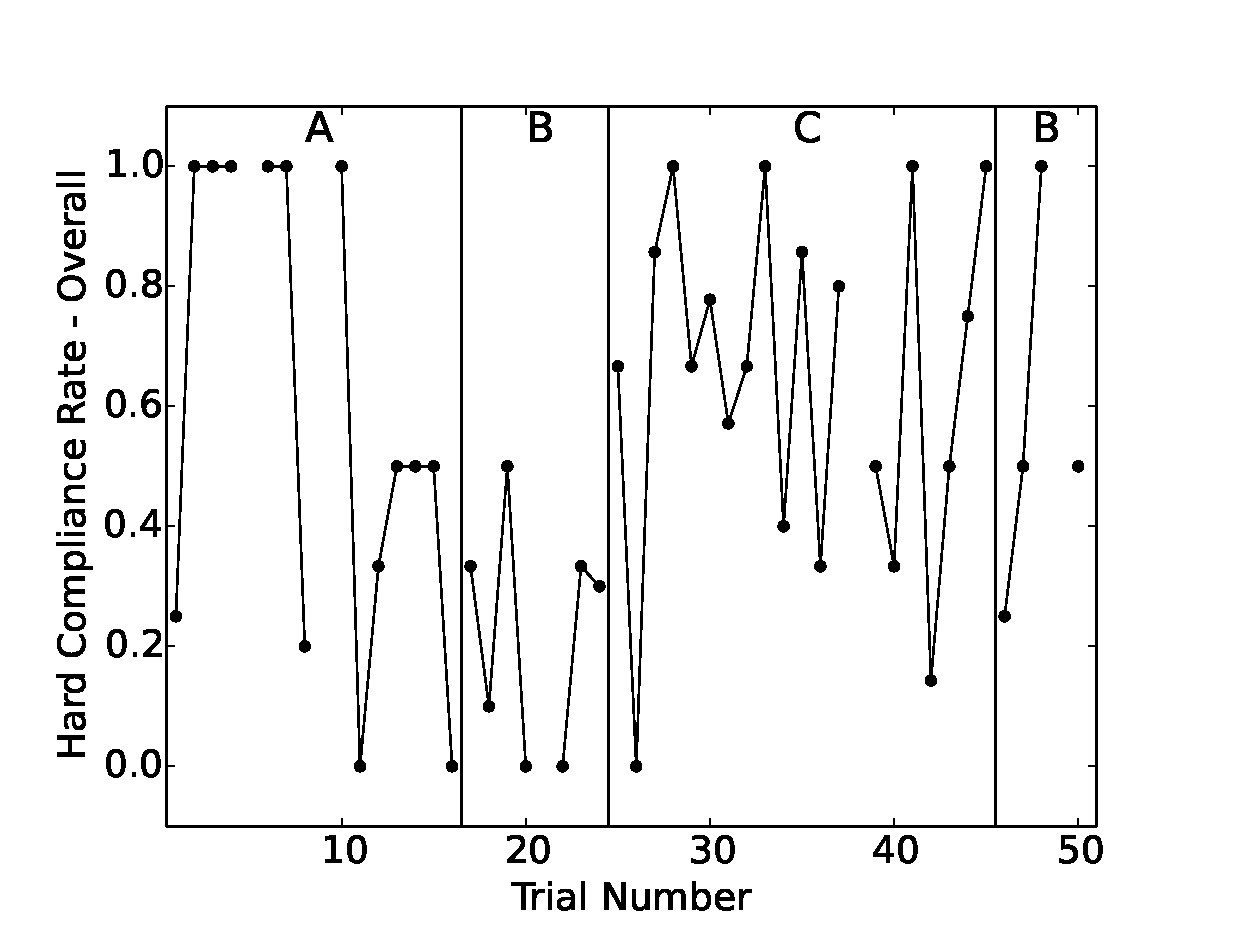
\includegraphics[width=1.1\linewidth]{./img/data_analysis/103HardComplianceRate-Overall.eps}
		\caption{Hard Compliance Rate - Overall}
		\label{fig:103HardComplianceRate-Overall}
	\end{subfigure}
	\hfill
	\begin{subfigure}[b]{0.49\textwidth}
		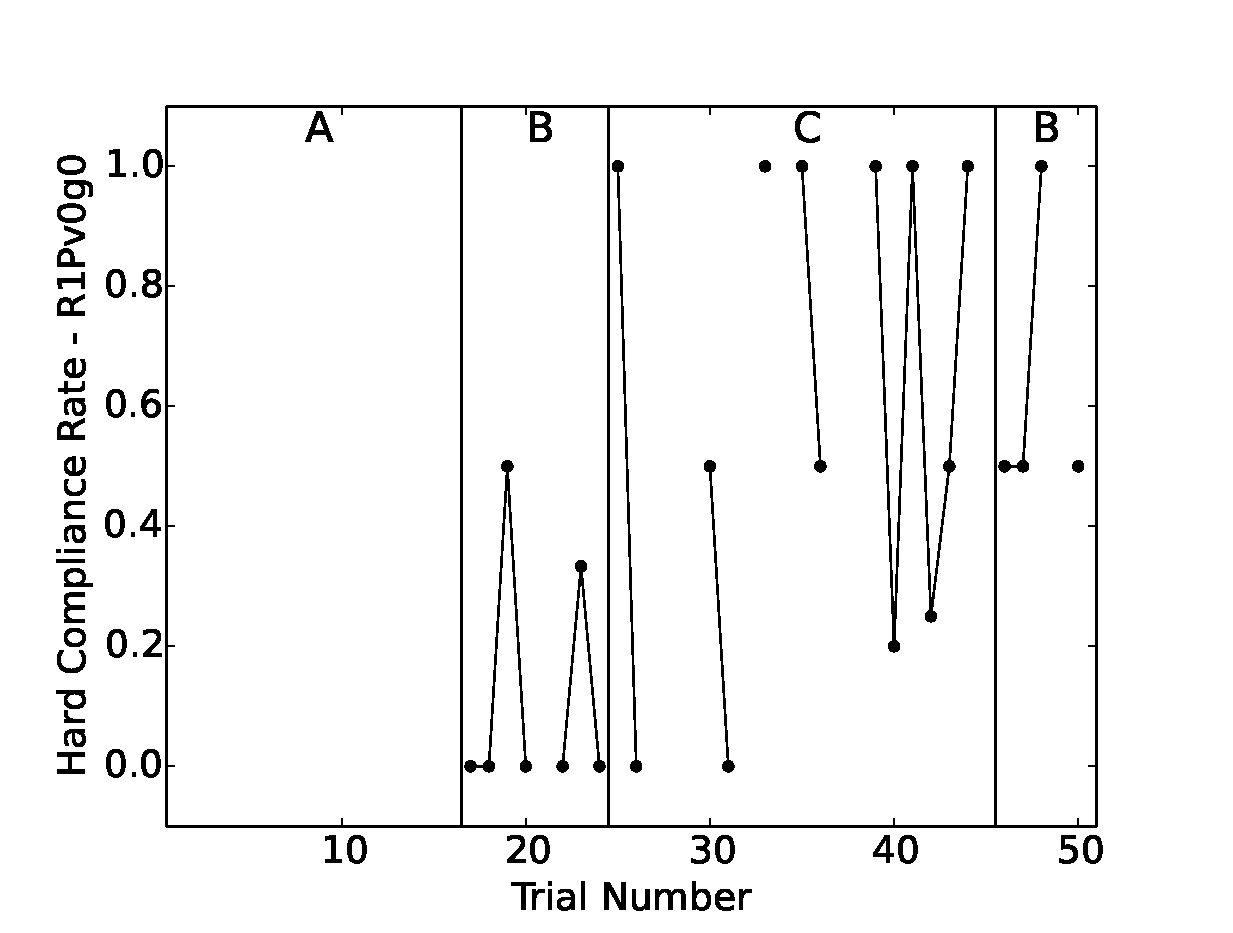
\includegraphics[width=1.1\linewidth]{./img/data_analysis/92HardComplianceRate-R1Pv0g0.eps}
		\caption{Hard Compliance Rate - Robot Only Prompts}
		\label{fig:92HardComplianceRate-R1Pv0g0}
	\end{subfigure}%
	\caption{Compliance Rate}
	\label{fig:ComplianceRate}
\end{figure}

\paragraph{Not Affected By Prompt Rate}
A response is counted towards ``not affected by prompt'' if the child was executing a wrong step and did not change after the prompt or was idling and did not change after the prompt.  The not affected by prompt rate is shown in Plot \ \ref{fig:99NotAffectedByPromptRate-Overall}.  We see that for most phases, it levels at 15\%, but for robot alone repeat phase (second Phase B) it is at 35\%.  This shows the robot prompts were ignored more when the robot was first introduced, but improves to an acceptable level through Phase C.
\begin{figure} [h]
	\centering
	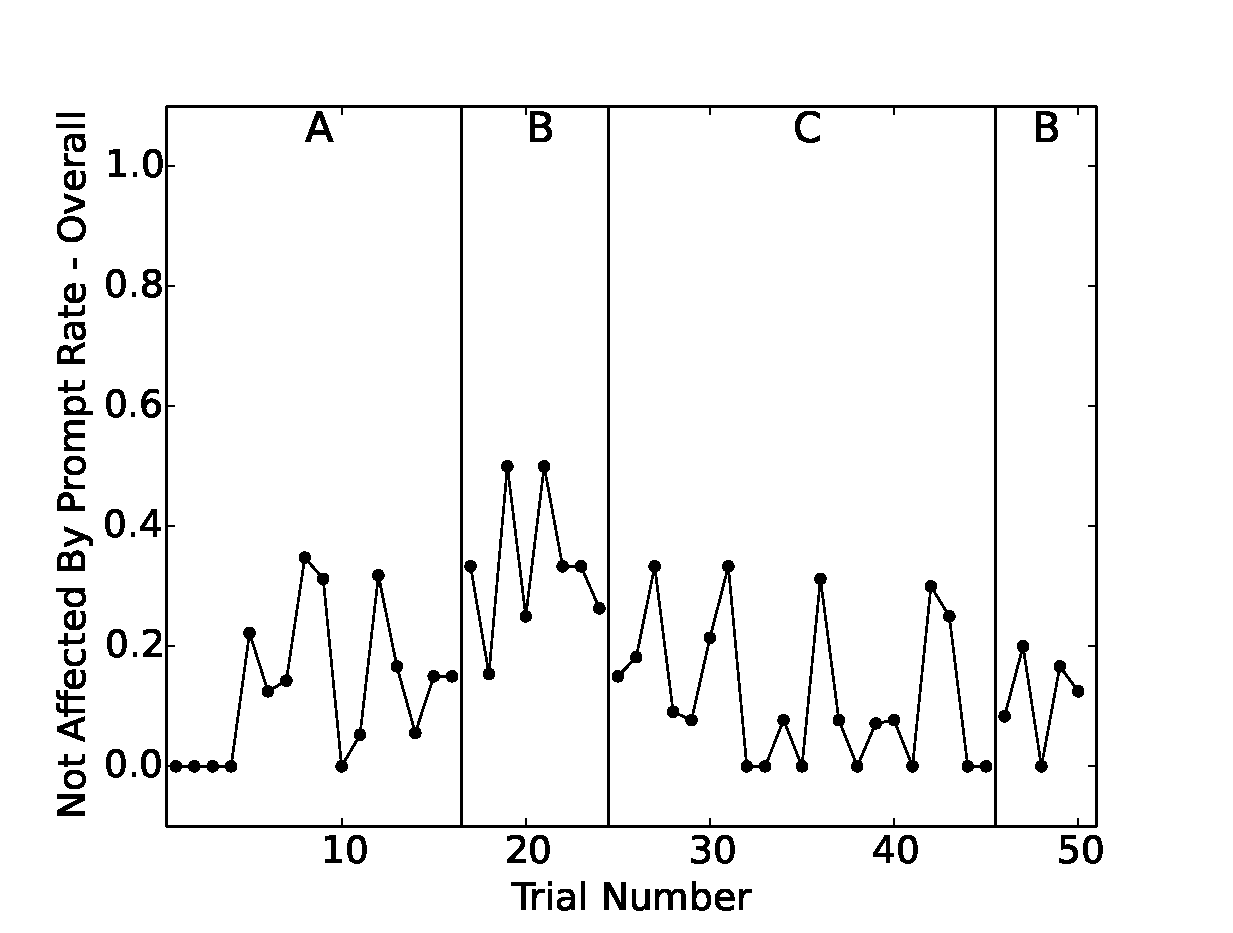
\includegraphics[width=0.6\textwidth]{./img/data_analysis/99NotAffectedByPromptRate-Overall.eps}
	\caption{Not Affected By Prompt Rate}
	\label{fig:99NotAffectedByPromptRate-Overall}
\end{figure}


\subsubsection{Engagement and Visual Attention}
To further characterize child's response to different prompting phases, we investigate how many times the child smiles and murmurs during step execution, and how often the child looks at the prompting agent during prompting and step execution.

\paragraph{Number of Times Child Smiles}
The measure "Total Number of Times Child Smiles" is shown in Plot \ \ref{fig:12TotalNumberofTimesChildSmiles}.  In it, parent alone phase (A) levels at 1.5, robot alone phase (first Phase B) levels at 0.5, robot parent phase (C) has a large spread and averages around 3, and robot alone repeat phase (second Phase B) also has a large spread and averages around 4.  It shows that the child smiles much more in later phases compared to earlier phases, and particularly, smiles in the repeat phase more than in robot alone phase.
\begin{figure} [h]
	\centering
	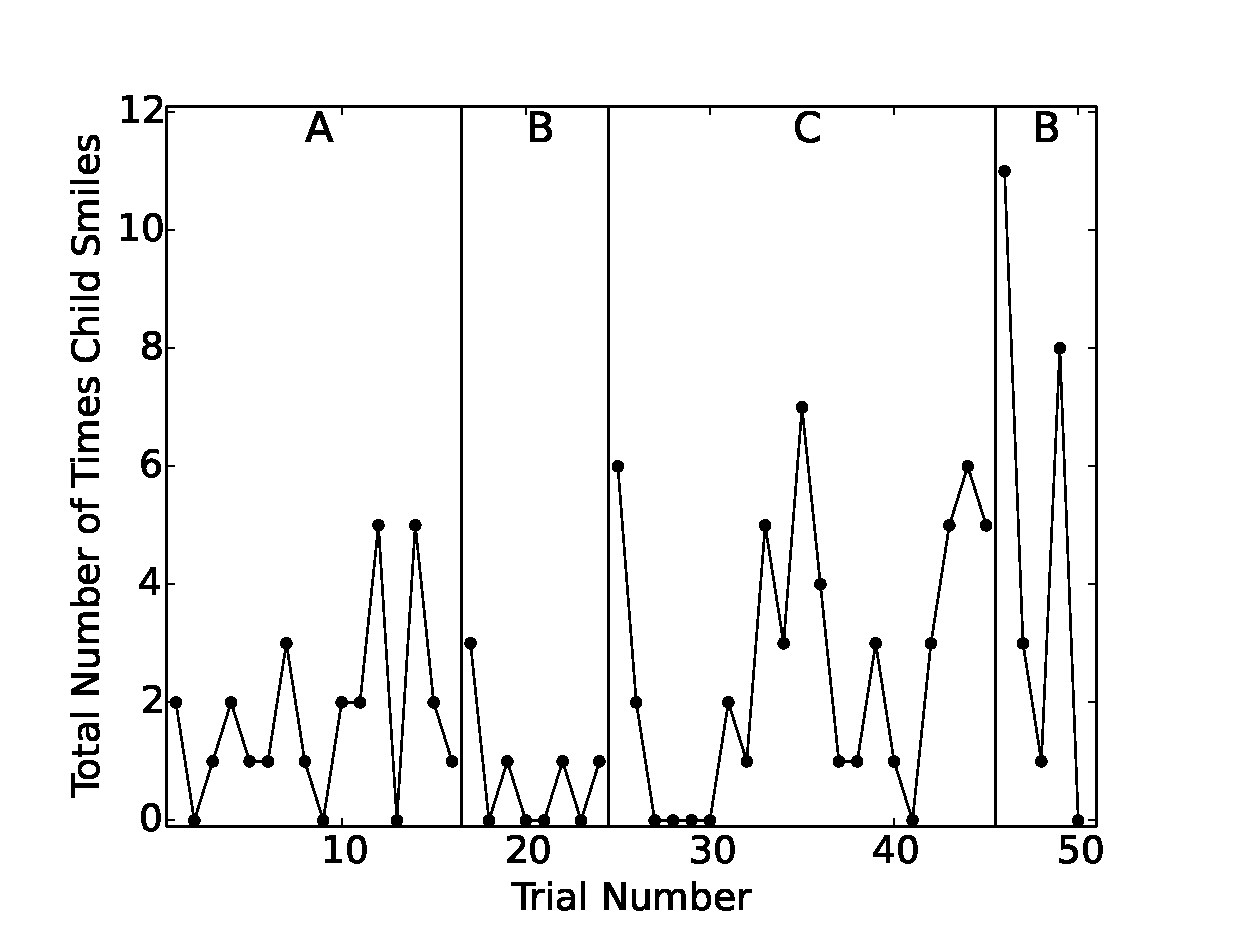
\includegraphics[width=0.6\textwidth]{./img/data_analysis/12TotalNumberofTimesChildSmiles.eps}
	\caption{Total Number of Times Child Smiles}
	\label{fig:12TotalNumberofTimesChildSmiles}
\end{figure}



\paragraph{Number of Times Child Murmurs}
The measure "Total Number of Times Child Murmurs" is shown in Plot \ \ref{fig:13TotalNumberofTimesChildMurmurs}.  In it, parent alone phase (A) has a large spread, averaging around 4.  Robot alone phase (first Phase B) levels at 0.5.  Robot parent phase (C) has a large spread, averaging around 4.  Robot alone repeat phase (second Phase B) levels at 2.  It shows that the child murmurs much more often when the parent is present.  Also, child murmurs in the repeat phase more than the robot alone phase.
\begin{figure} [h]
	\centering
	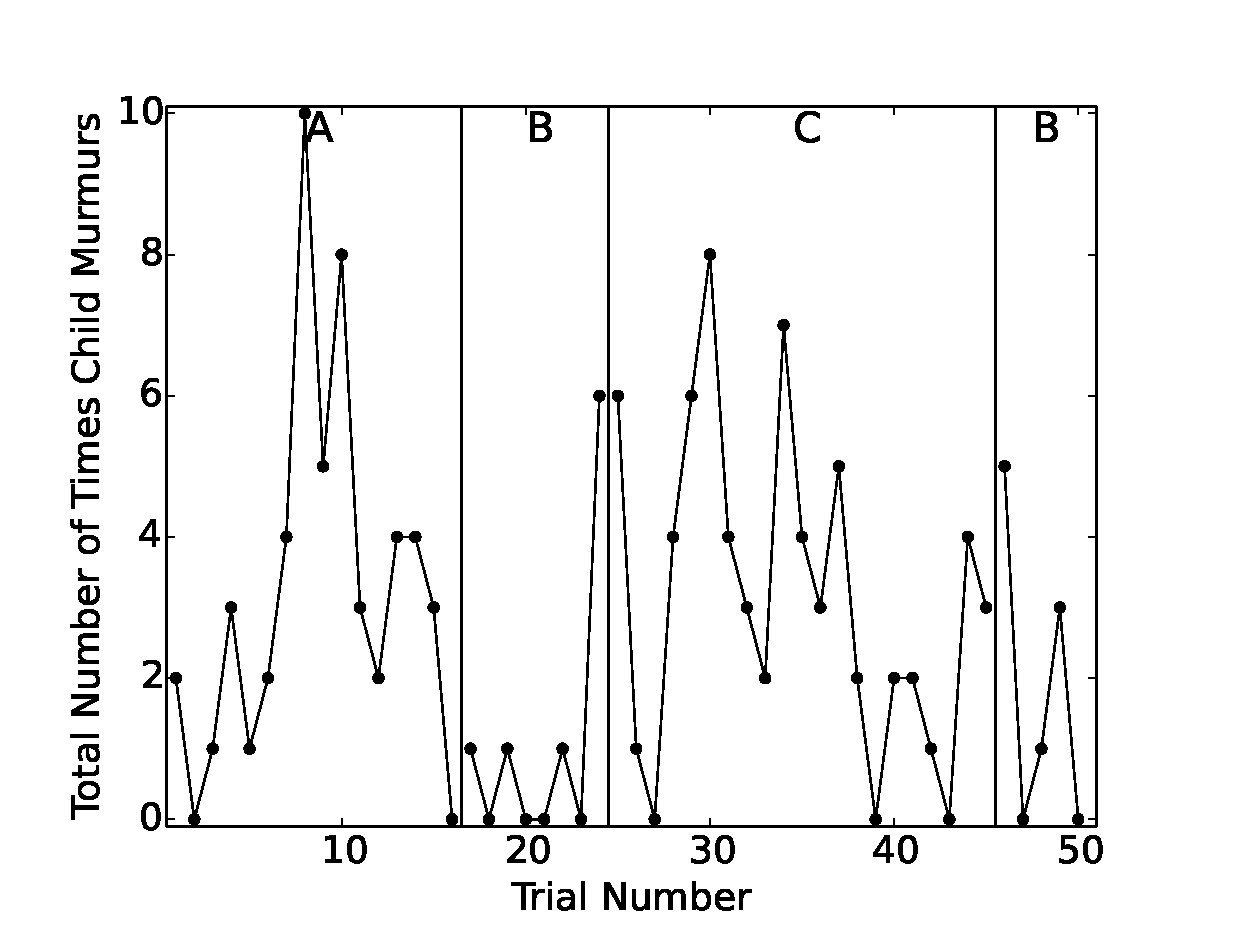
\includegraphics[width=0.6\textwidth]{./img/data_analysis/13TotalNumberofTimesChildMurmurs.eps}
	\caption{Total Number of Times Child Murmurs}
	\label{fig:13TotalNumberofTimesChildMurmurs}
\end{figure}

\paragraph{Looking at Prompting Agent Rate}
A prompt can be given by the parent, by the robot, or by them together.  During prompting and during step execution, the child may turn and look at the parent and/or the robot.  The gaze behavior of the child is shown in Figure \ref{fig:LookingAtPromptingAgentDuringPrompts} for all the cases above.  Because not all cases have the same amount of data in all phases, we will only mention here the phases that have enough evidence.  In Plot \ref{fig:8LookingatParentRateGivenParentPrompted}, ``Looking at Parent Rate - Given Parent Prompted'' levels at 40\% in parent alone phase (A).  In Plot \ref{fig:92HardComplianceRate-R1Pv0g0}, ``Looking at Robot Rate - Given Robot Prompted'' trends downward from 50\% to 30\% for robot alone phase (first Phase B), levels at 30\% with high spread for robot parent phase (C), and levels at 20\% for robot alone repeat phase (second Phase B).  We see that when the parent and the robot prompt individually, the parent has a higher chance of getting the child's visual attention.  Although the robot had similar levels of attention when was first introduced, it dropped as the study went on.  In Plot \ref{fig:10LookingatParentRateGivenBothPrompted}, ``Looking at Parent Rate - Given Both Prompted'' averages around 50\% with high spread in robot parent phase (C).  In Plot \ref{fig:11LookingatRobotRateGivenBothPrompted}, ``Looking at Robot Rate - Given Both Prompted' levels at 15\% for robot parent phase (C).  We see that when the parent and the robot prompt at the same time, the parent had a greater amount of visual attention.  It is interesting to note that the parent had similar levels of visual attention when prompting alone and when prompting with the robot.  The robot, however, experienced a decrease in visual attention level when the parent prompts with it.
\begin{figure}[h]
	\centering
	\begin{subfigure}[b]{0.49\textwidth}
		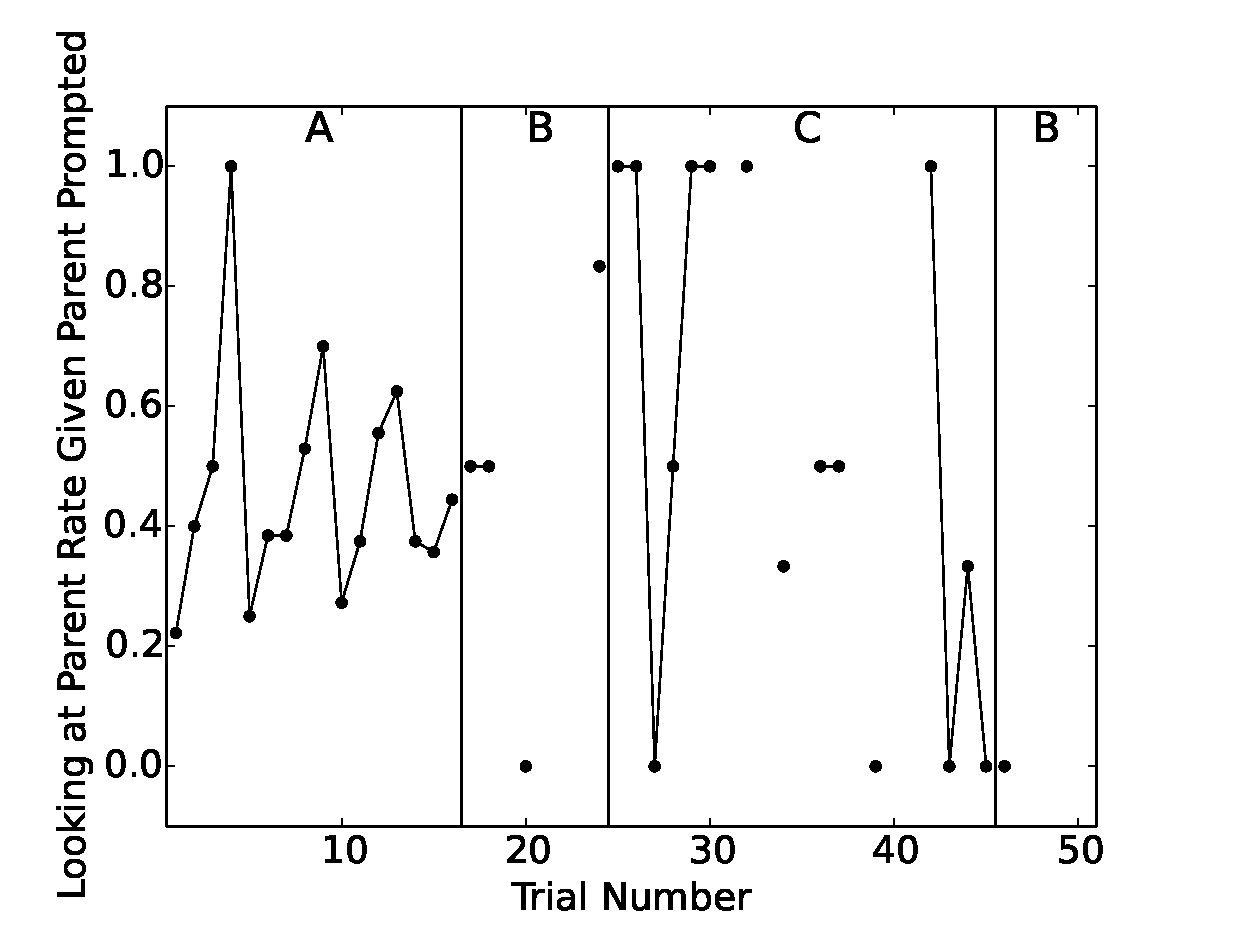
\includegraphics[width=1.1\linewidth]{./img/data_analysis/8LookingatParentRateGivenParentPrompted.eps}
		\caption{Looking at Parent Rate - Given Parent Prompted}
		\label{fig:8LookingatParentRateGivenParentPrompted}
	\end{subfigure}
	\hfill
	\begin{subfigure}[b]{0.49\textwidth}
		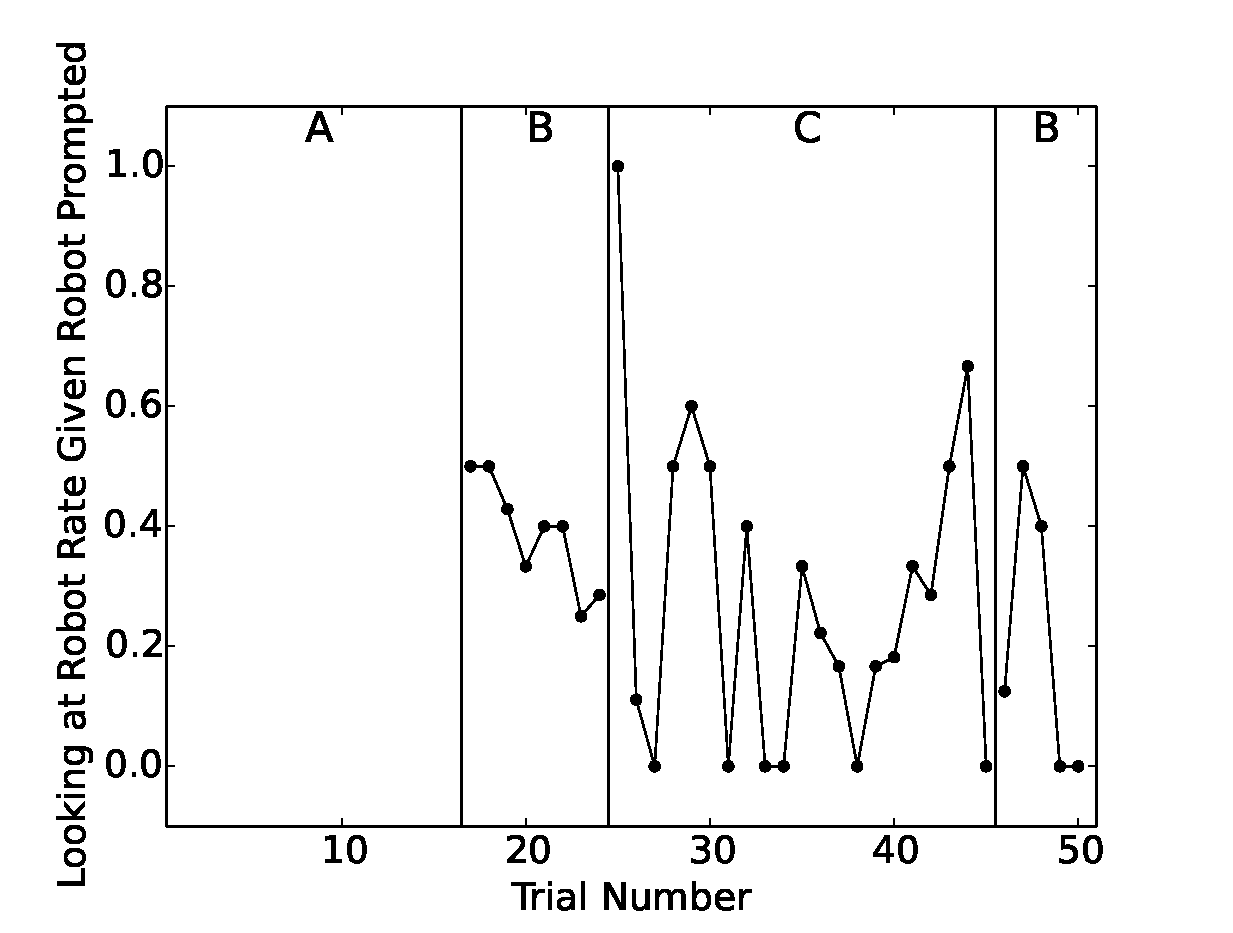
\includegraphics[width=1.1\linewidth]{./img/data_analysis/9LookingatRobotRateGivenRobotPrompted.eps}
		\caption{Looking at Robot Rate - Given Robot Prompted}
		\label{fig:9LookingatRobotRateGivenRobotPrompted}
	\end{subfigure}%

	
	\begin{subfigure}[b]{0.49\textwidth}
		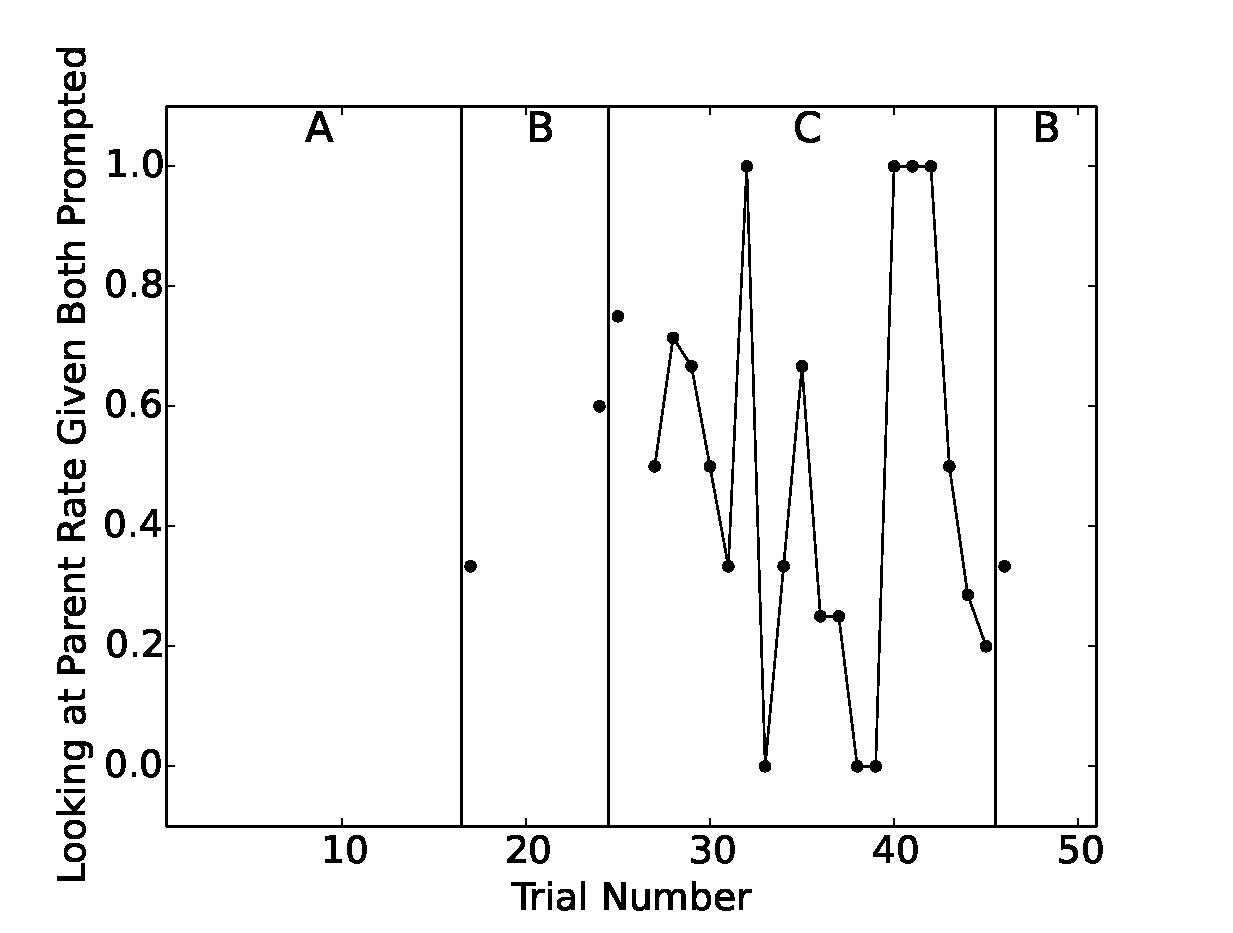
\includegraphics[width=1.1\linewidth]{./img/data_analysis/10LookingatParentRateGivenBothPrompted.eps}
		\caption{Looking at Parent Rate - Given Both Prompted}
		\label{fig:10LookingatParentRateGivenBothPrompted}
	\end{subfigure}
	\hfill
	\begin{subfigure}[b]{0.49\textwidth}
		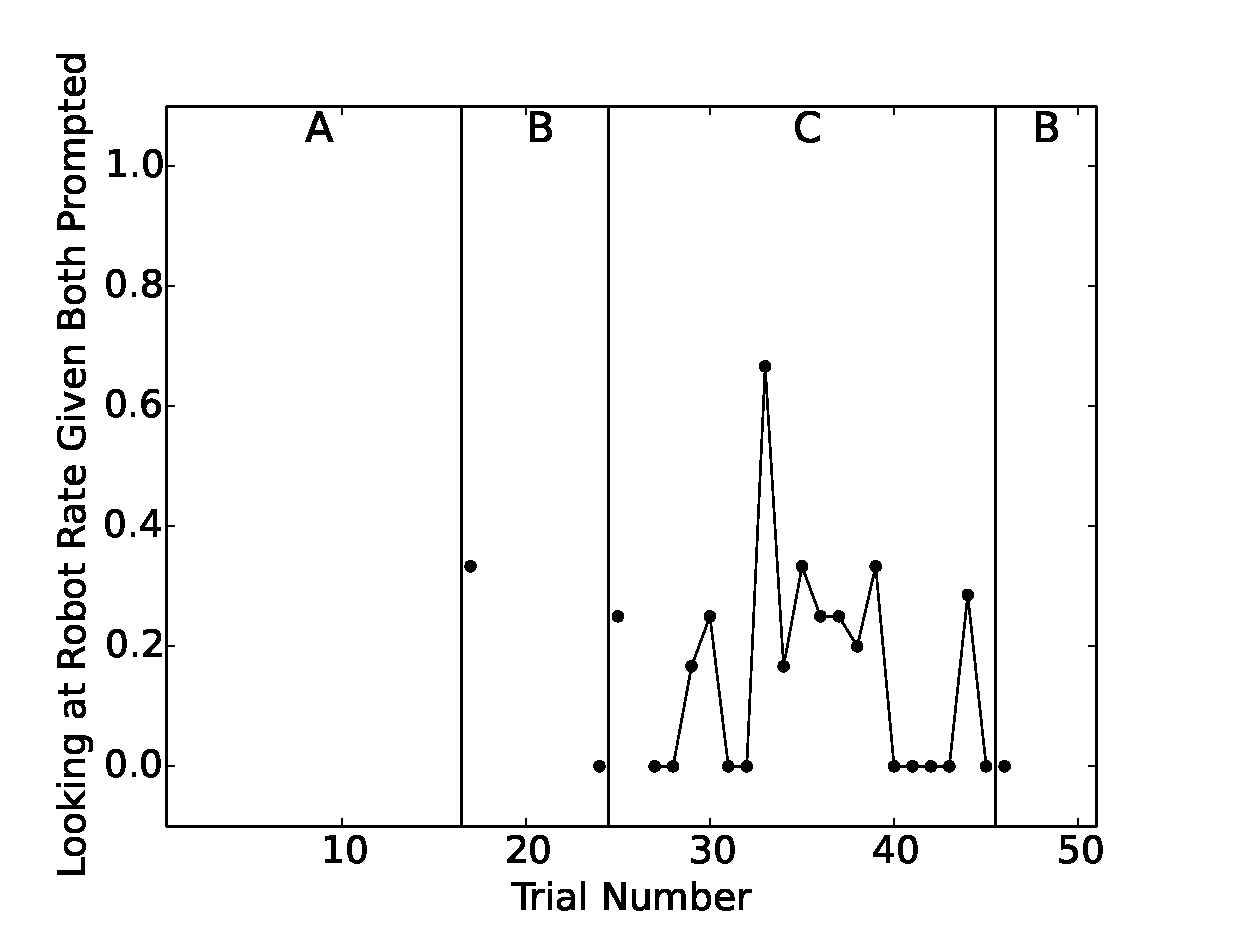
\includegraphics[width=1.1\linewidth]{./img/data_analysis/11LookingatRobotRateGivenBothPrompted.eps}
		\caption{Looking at Robot Rate - Given Both Prompted}
		\label{fig:11LookingatRobotRateGivenBothPrompted}
	\end{subfigure}%
	\caption{Looking at Prompting Agent Rate}
	\label{fig:LookingAtPromptingAgentDuringPrompts}
\end{figure}

\subsection{Survey Data Results}

\subsubsection{Entrance Survey}
The entrance survey results are reported as follows:

\paragraph{Child's Experience with Technologies}
The child is more of a visual learner.  He uses a computer at home, and likes to use it very much.  He also likes to use other technologies (e.g. iPhone, iPad), and likes to watch movies and TV.  He doesn't have a robot toy to play with at home or at school, so the parent doesn't know how much he likes to play with robot toys.  The parent never used technologies to help the child with self-care activities except using pictures to teach step by step hand-washing.

\paragraph{Child's Personal Preferences}
The child is sensitive to sound.  He likes Disney cartoon musics, and likes to watch his favorite cartoon scenes repeatedly on the iPad.  To reward the child after a good behavior, the parent suggested the following rewards: give extra time to play on iPad, give him praises (e.g. good job), give children books to read and animal dinosaurs to play with, give the parent's iPhone since his favorite musics are on there.

\paragraph{Child's Abilities on Hand-washing and on Other ADLs}
The parent agrees that the child usually gets distracted when performing hand-washing.  To assist him, the parent mainly reminds him to put soap, rinse properly, and dry properly with towel.  He needs more prompting in these areas since he always washes in a hurry.

Other activities the child needs help with include:  tooth brushing -- 2 hours/week; bathing -- 4.5 hours/week; dressing -- usually just hand the clothes to him, he knows how to put them on, but needs reminders of the order of the clothing, 7 hours/week.

\paragraph{Parent's Expectation and Concerns}
The parent expected the robot to be helpful in reminding the child to put soap, rinse and dry more, similar to the role of the parent.  Some concerns the parent has include: the child may be wondering why does he need to wash hands so many times repeatedly; the child performs well in his comfort zone with the same environment, so it takes a while for the child to get used to the lab environment.


\subsubsection{Post-Intervention Survey for Parent}
The post-intervention survey results are presented in Table \ref{tab:PostInterventionSurveyData}.  We see that the parent was happy with all aspects of the robot as a prompting agent, but did not see it to be as good as herself yet.  The suggestions the parent made regarding the robot and the experiment are reported in the discussion section.

\begin{table}[h]
	\centering
	\begin{tabular}{ | p{12cm} | l | }
		\hline
		\textbf{Survey Question}	&	\textbf{Parent's Answer}	\\	\hline	\hline		
		Hand-washing steps break down was appropriate	&	Strongly Agree	\\	\hline
		My child understood the verbal prompts	&	Agree	\\	\hline
		Robot's verbal prompts were appropriate	&	Strongly Agree	\\	\hline
		The prompt wordings were similar to mine	&	Strongly Agree	\\	\hline
		The prompt voice and tone were appropriate	&	Strongly Agree	\\	\hline
		The prompt wordings were easy to understand	&	Strongly Agree \\	\hline
		My child understood the gesture prompts	&	Strongly Agree	\\	\hline
		The gesture prompts were appropriate	&	Strongly Agree	\\	\hline
		The gesture prompts were easy to understand	&	Agree	\\	\hline
		The physical appearance of robot is aesthetically pleasing	&	Agree	\\	\hline
		The attention grabber gestures were appropriate	&	Strongly Agree	\\	\hline
		The verbal rewards were appropriate	&	Strongly Agree	\\	\hline
		The reward gestures were appropriate	&	Strongly Agree	\\	\hline
		The robot was effective in assisting my child through hand-washing	&	Strongly Agree	\\	\hline
		The robot motivated my child to wash hands	&	Strongly Agree	\\	\hline
		The robot was fun for my child to use	&	Strongly Agree	\\	\hline
		My child was confused by the robot	&	Disagree	\\	\hline
		I like the idea of a robot prompting my child	&	Strongly Agree	\\	\hline
		The robot is able to provide guidance as well as I can or better	&	Neither Agree or Disagree	\\	\hline
		I would want to own a robot like this one	&	Strongly Agree	\\	\hline
	\end{tabular}
	\caption{The Post-Intervention Survey Data}
	\label{tab:PostInterventionSurveyData}
\end{table}
\section{Discussion}
A Wizard of Oz study has been conducted following the A-B-C-B design.  In Phase A, the parent alone prompted the child through hand-washing steps.  In first Phase B, the robot alone prompted the child.  In Phase C, the parent and the robot jointly prompted.  Visual analyses were used to analyze the measures from annotated video data of the trials.

%To evaluate the effectiveness of the robot prompts on child's step completion, to measure the child's compliance to the prompts, and to investigate their relationships with the child's engagement level during hand-washing, the following metrics are calculated and analyzed from the video data annotations for each trial:

%- was the robot more effective in guiding child to complete steps than the parent?
%- does the child respond to the robot equally well as to the parent?
%- is it because child is not engaged?  or is it because robot prompts not understandable? or is it because robot not as authoritative as the parent? or is it something else? (like not responsive enough, or not contingent to child's behaviour enough?)

\subsection{Primary Results}
We saw that having the robot present in the washroom contributed positively in increasing the Number of Complete Steps.  Comparing with the parent's prompts' contribution, the robot prompts had the similar size of contribution in the first Phase B, smaller size in Phase C, and bigger size in the second Phase B.  It is interesting that the robot had drastically greater contribution in the second Phase B (increase of 1.5), but not in the first (increase of 0.5).  We believe this is mainly due to the child learning to follow the robot after going through Phase C, where the parent jointly prompted with the robot, telling the child to follow the robot's prompts.  Although robot prompts in the second Phase B (increase of 1.5) did not arrive at the same effectiveness as that of the parent's in Phase A (increase of 3), we believe that, given sufficient Phase C training, the robot potentially could replace the parent as an independent prompting agent.

Another way to look at the robot prompts' effectiveness is this: We first observe that the Number of Incomplete Steps are kept near zero in all trials through either parent prompts or robot prompts or joint (Number of Incomplete Steps is shown in Figure \ref{fig:4NumberofIncompleteSteps}).  In addition, we saw that the Number of Parent Prompts - Overall was sharply reduced in both of B phases (when robot prompted alone) and experienced a continual reduction in Phase C when robot and parent jointly prompted.  This shows two things: First, in the two B phases, the robot was able to guide the child through hand-washing without constant parent supervision.  Second, in Phase C, when the parent jointly prompts with the robot to have the child better follow the robot, the parent was able to gradually fade out the prompts while keeping Number of Incomplete Steps near zero since the child listened to the robot more and more.
\begin{figure} [h]
	\centering
	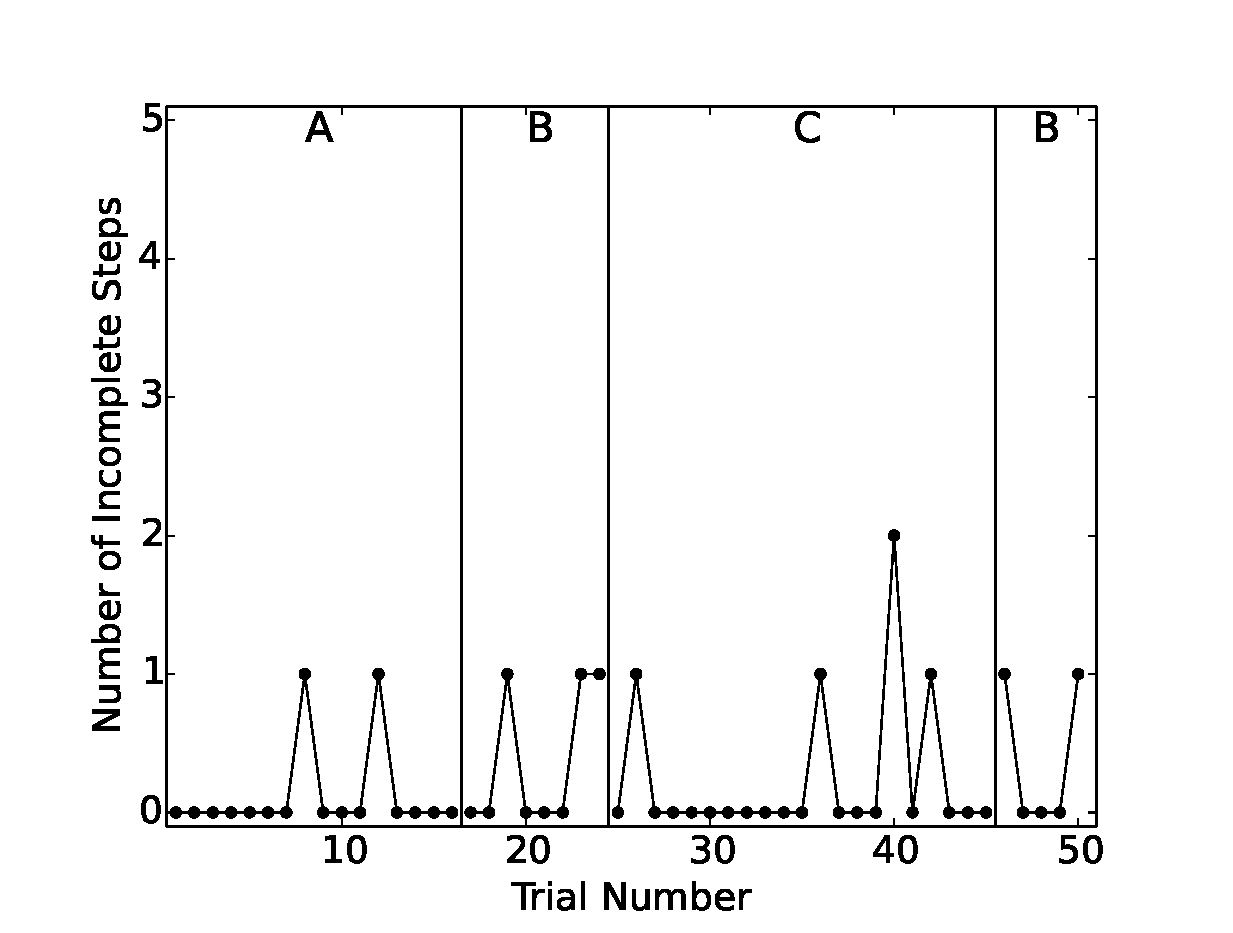
\includegraphics[width=0.6\textwidth]{./img/data_analysis/4NumberofIncompleteSteps.eps}
	\caption{Number of Incomplete Steps}
	\label{fig:4NumberofIncompleteSteps}
\end{figure}

One major limitation of evaluating robot prompt effectiveness based on the above measures (i.e. Number of Complete Steps and Number of Parent Prompts) is that we could have a trial where the child may be ignoring robot prompts and skipping steps.  This would fluctuate the total number of steps, and thus fluctuating Total Number of Complete Steps as well, influencing the estimation of effectiveness of robot vs. parent prompts.  Such fluctuation is not detectable using the measure Number of Parent Prompts, either.  Our study did not employ a strict hand-washing steps ordering that the child must adhere to, and we left it up to the parent's discretion to intervene as they think the child needs.  As a result, the measure Number of Parent Prompts does not fully reflect child skipping steps either.  One way to circumvent this problem may be to define a step order before hand, and monitor the measure Total Number of Steps Skipped each trial to characterize its effects.  However, it seems that children with ASD, or at least the one participant we had, had strict preference on the order of hand-washing steps, and the order is not known a priori and may be different across individuals.  Thus, having a flexible prompting scheme in terms of step orders is preferred.  However, this means that the decision of what steps need to be executed, and hence which steps were missed, often depends on the sequence of steps executed thus far in a trial.  This makes it troublesome to define what is meant by missed steps, possibly making the analysis process unfeasible.  Another way to circumvent this problem is to use other measures that reflect the child skipping steps, or not following the step order prompted -- the Compliance Rate and Not Affected By Prompt Rate measures can be used for this purpose.

We saw that both Compliance Rate and Hard Compliance Rate are high in Phase A, C, and second Phase B, and low in the first Phase B.  The contrary pattern exists for Not Affected By Prompt Rate.  This means that the prompts in the first Phase B were complied much less often, and a large portion of that noncompliance was exhibited as the child ignoring the prompts and kept doing some other step or not doing any step at all.  At the same time, both the Total Number of Complete Steps - With Robot and Parent Prompts and the Number of Parent Prompts - Overall are low in the first Phase B while the Number of Incomplete Steps in that phase is still near zero.  This is precisely the scenario talked about earlier, where the child skips many steps while the parent did not enforcement the steps skipped through prompts.  Thus, it is apparent that the robot was only effective in the second Phase B, but not in the first Phase B.  We believe the difference between first and second Phase B is that second Phase B is after Phase C, and first Phase B is before Phase C.  Phase C functioned as a training phase and helped the child comply better to robot prompts.

There are also other differences that existed between first and second Phase B, so training Phase C may not be the reason (or may not be the sole reason) for improved effectiveness of robot prompts in the second Phase B.  One important change happened to the way the robot was controlled starting at the seventh trial of first Phase B.  We found out, after introducing the robot to the child and conducting six trials, that the child did not follow the order of steps prompted by the robot.  This meant the robot needed to change the order of steps being prompted on the fly quickly.  However, due to the way its remote control was programmed, the researcher cannot change prompts quickly enough, resulting in the child growing impatient and ignored the robot prompts altogether.  Thus, the robot remote control scheme was changed from being inflexible in step order into one that the researcher can select the current prompting step on the fly.  Also, instead of implementing a timer, and automatically issuing the prompt after a predefined seconds of waiting, the timing of prompt delivery was changed to be decided by the researcher on the fly.  This makes the robot behavior much more flexible and relevant to the child's behaviors.  This robot control scheme change affected the last two trials in the first Phase B, and all trials in the second Phase B and Phase C.  This change, however, did not cause any abrupt change in any of our measures (comparing the last two trials of first Phase B with the previous trials in the phase).  Thus, we believe the robot control scheme change was not the cause of the improved effectiveness of robot prompts in the second Phase B.

It is important to mention here that the parent did not prompt the same way uniformly through Phase C, but instead was involved in various degrees.  The level of involvement was left up to the parent's discretion for each trial, with the ultimate goal to fade out the involvement to minimal by the end of Phase C.  By reviewing how the parent prompted the child, five levels of involvement were observed:
\begin{itemize}
	\item \textbf{Level 0}: the parent is outside of the room out of the child's view, only comes into the washroom to prompt when the child is not following the robot (this behavior is similar to that during Phase B)
	\item \textbf{Level 1}: the parent stands beside the child in the washroom, and mainly uses gestures to prompt the child to follow the robot and to demonstrate the step's motions after robot prompts
	\item \textbf{Level 2}: the parent stands beside the child in the washroom, and uses both verbals and gestures to prompt the child about each hand-washing steps, in competition to the robot prompts
	\item \textbf{Level 3}: the parent stands behind the child, and physically guide the child to follow the robot prompts
	\item \textbf{Level 4}: the parent stands beside the child, and prompts as the parent sees fit each hand-washing steps, with no robot present
\end{itemize}
The Parent Involvement Level is plotted in Figure \ref{fig:107ParentInvolvement}.  We see that, in Phase C, the parent mainly alternated between trial segments of level 1 and level 3 to train the child to follow the robot, while mixing single trials of level 0 to monitor the child's progress when left with robot alone.
\begin{figure} [h]
	\centering
	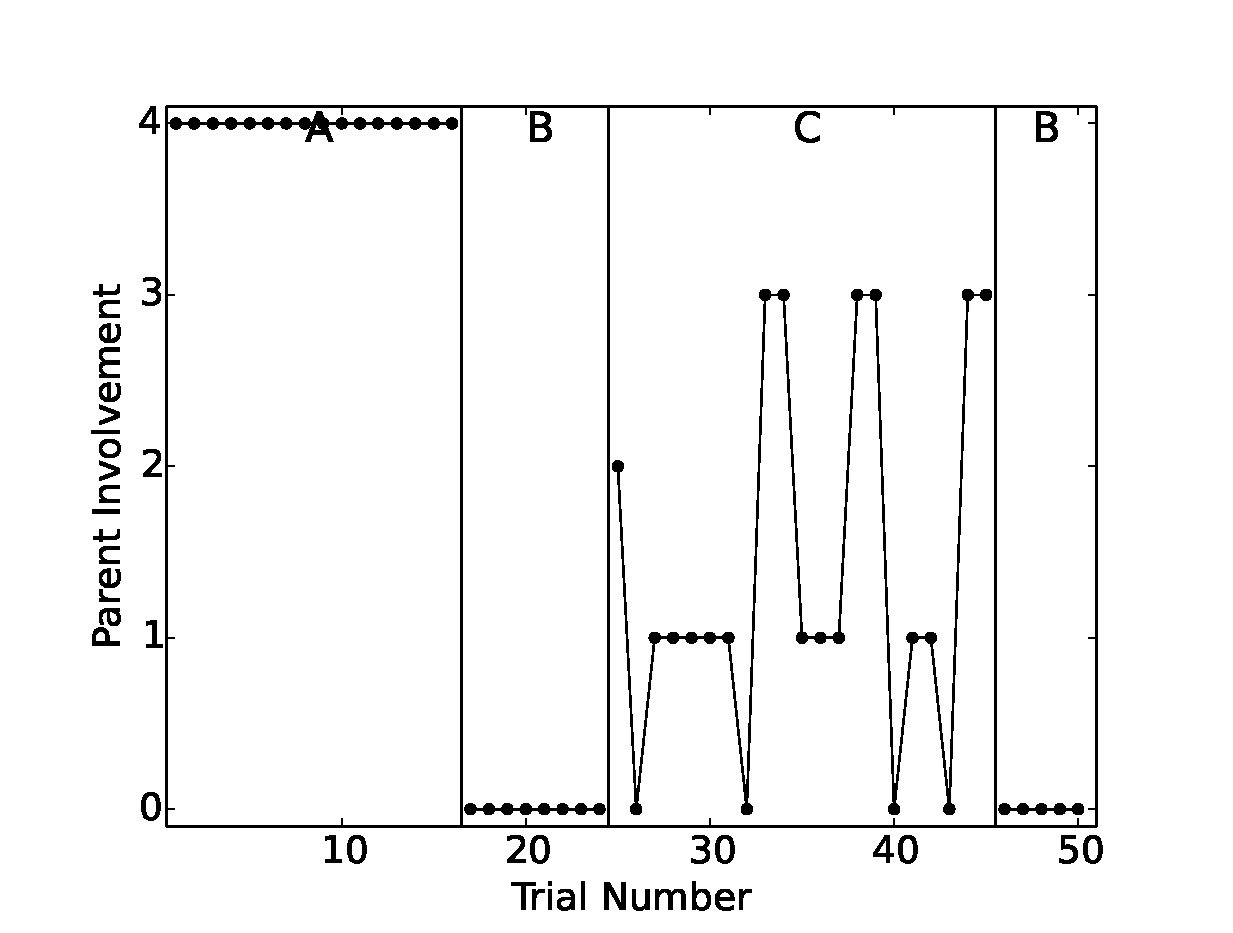
\includegraphics[width=0.6\textwidth]{./img/data_analysis/107ParentInvolvement.eps}
	\caption{Parent Involvement}
	\label{fig:107ParentInvolvement}
\end{figure}

With this in mind, we can attempt to answer what happened in Phase C that resulted in an increase of robot prompts effectiveness in the second Phase B.  The first observation we can make is by plotting only the level 0 parent involvement trials, where the robot is left alone with the child.  The Compliance Rate and Hard Compliance Rate for robot alone trials is shown in Figure \ref{fig:ComplianceRate_robotAloneOnly}.  The Not Affected By Prompt Rate for robot alone trials is shown in Figure \ref{fig:99NotAffectedByPromptRate-Overall_robotAloneOnly}.  We see a sharp jump rather than a gradual change in both Compliance Rate and Not Affected By Prompt Rate when we move from first Phase B to Phase C.  This suggests that the cause of effectiveness improvement of robot prompts was probably not a gradual processes such as the child learning hand-washing or getting used to the robot or washroom environment.  Instead, it was a sudden event experienced at the start of Phase C -- the joint prompting from the parent telling the child to follow the robot.  We also believe that, although the improvement in robot prompt effectiveness was immediate, a longer training Phase C was needed for the child to retain the behavior.  Note that Hard Compliance Rate did not show immediate change in levels.  This is possibly due to its low sample size, since hard compliance scenarios (child attempted a step before prompt and then was prompted for another step) were not that abundant.
\begin{figure}[h]
	\centering
	\begin{subfigure}[b]{0.49\textwidth}
		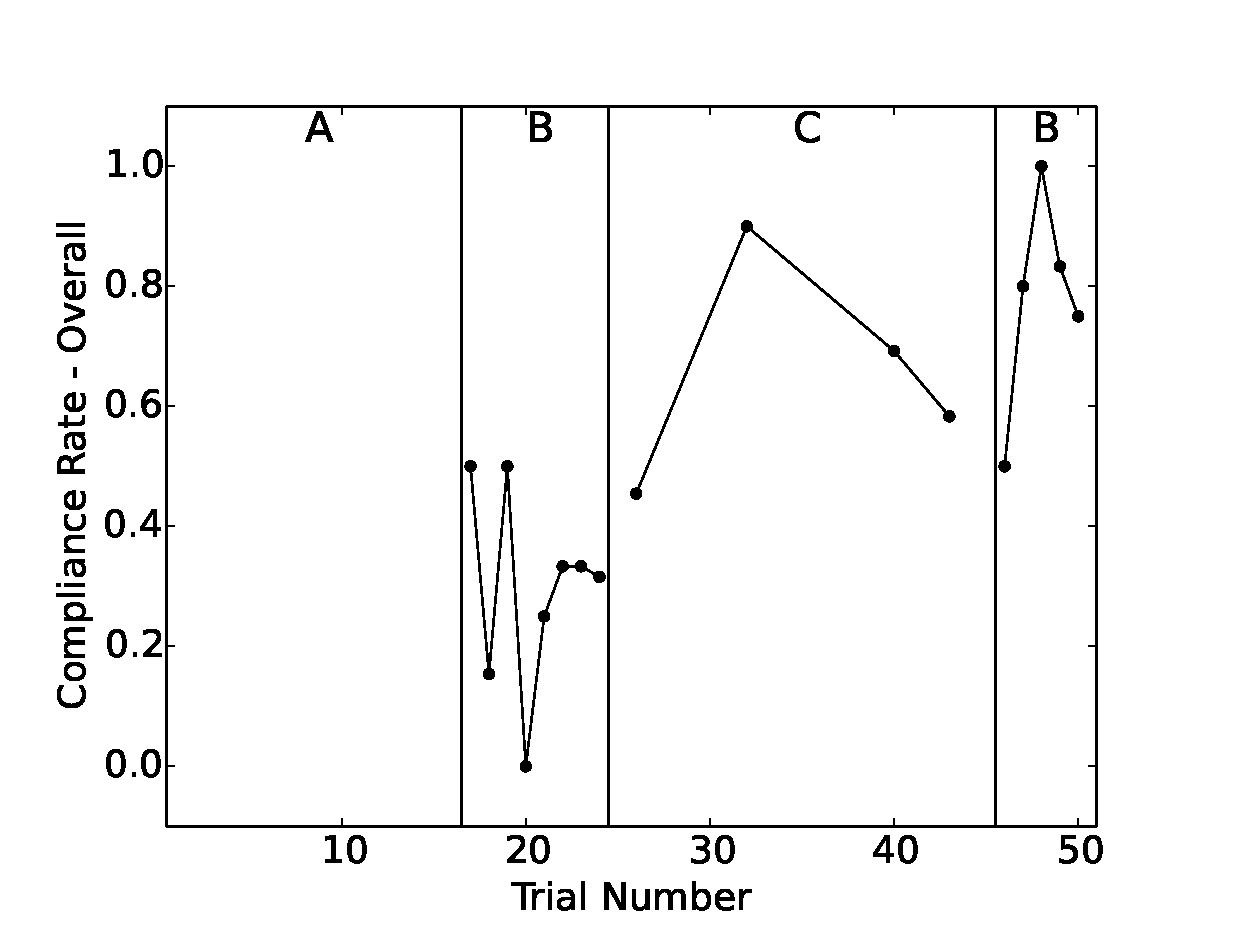
\includegraphics[width=1.1\linewidth]{./img/data_analysis/102ComplianceRate-Overall_robotAloneOnly.eps}
		\caption{Compliance Rate - Overall - Robot Alone Trials}
		\label{fig:102ComplianceRate-Overall_robotAloneOnly}
	\end{subfigure}
	\hfill
	\begin{subfigure}[b]{0.49\textwidth}
		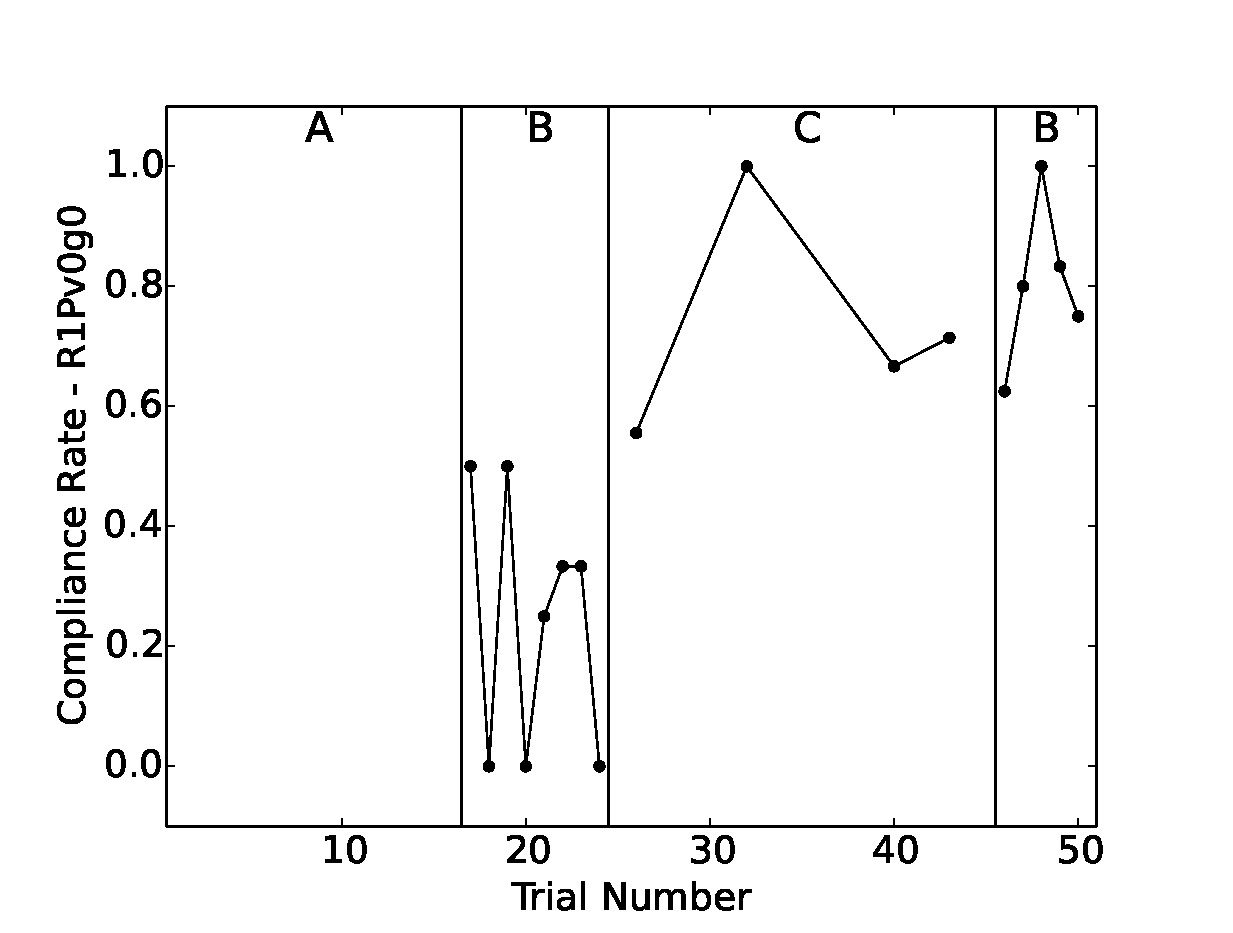
\includegraphics[width=1.1\linewidth]{./img/data_analysis/79ComplianceRate-R1Pv0g0_robotAloneOnly.eps}
		\caption{Compliance Rate - Robot Only Prompts - Robot Alone Trials}
		\label{fig:79ComplianceRate-R1Pv0g0_robotAloneOnly}
	\end{subfigure}%

	
	\begin{subfigure}[b]{0.49\textwidth}
		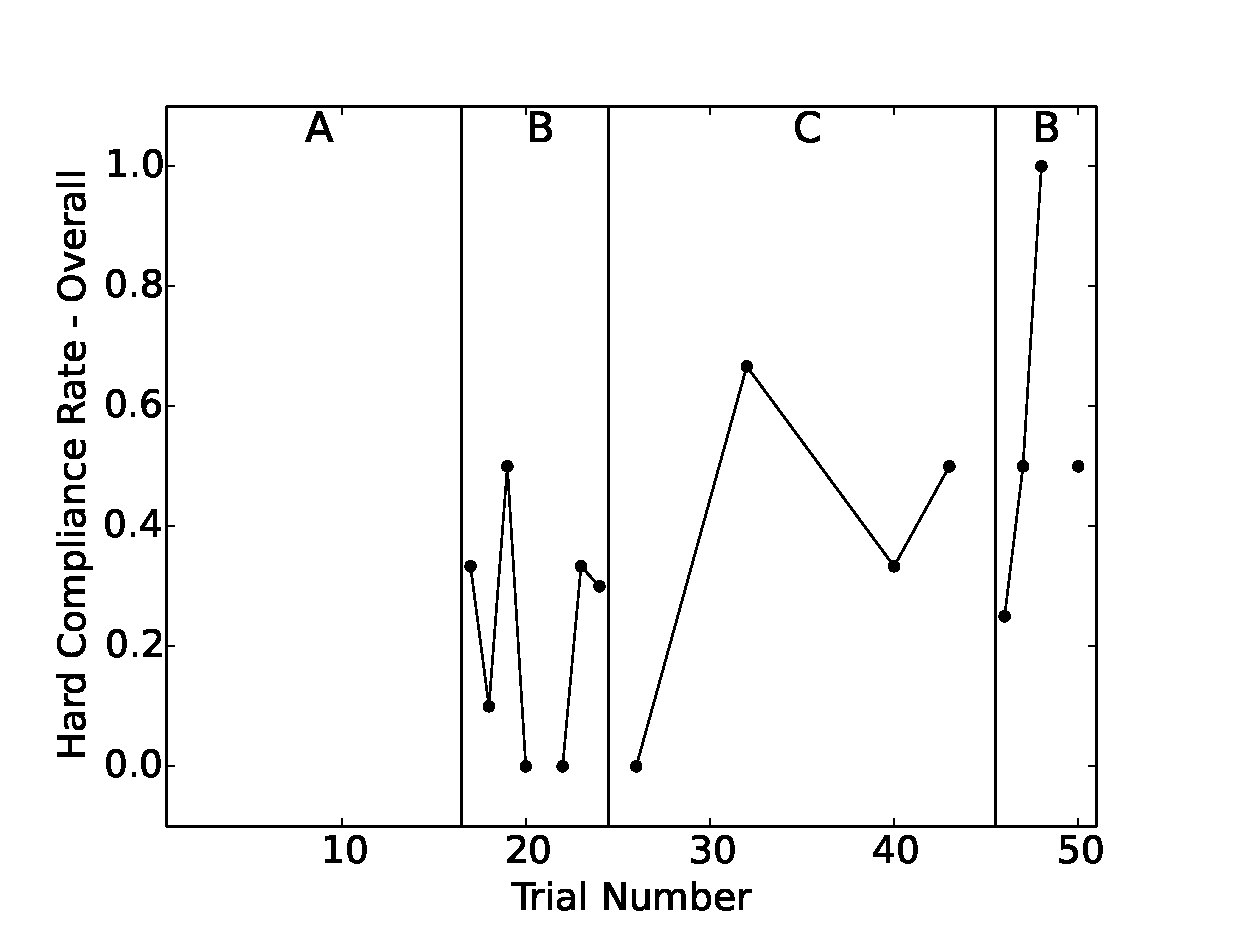
\includegraphics[width=1.1\linewidth]{./img/data_analysis/103HardComplianceRate-Overall_robotAloneOnly.eps}
		\caption{Hard Compliance Rate - Overall - Robot Alone Trials}
		\label{fig:103HardComplianceRate-Overall_robotAloneOnly}
	\end{subfigure}
	\hfill
	\begin{subfigure}[b]{0.49\textwidth}
		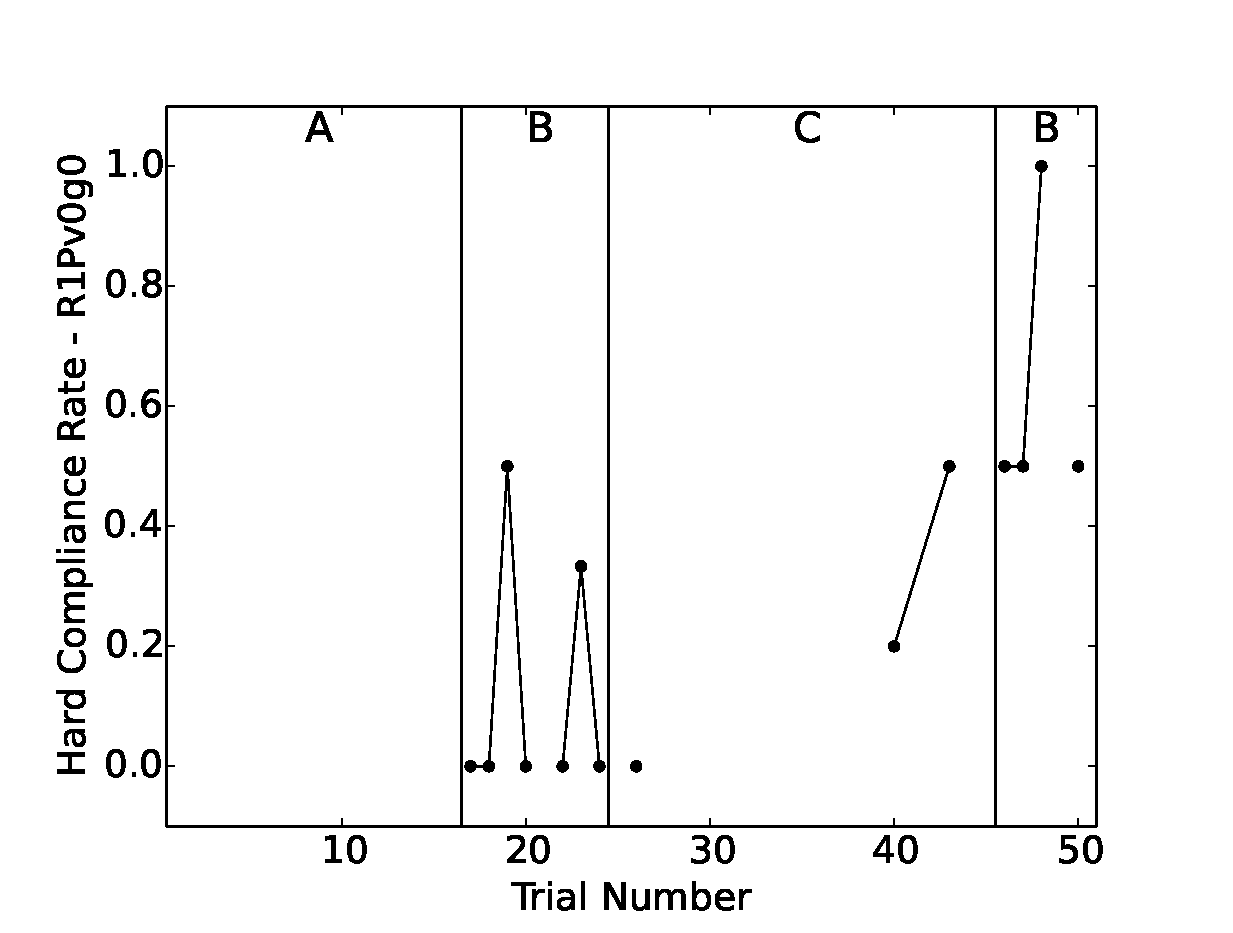
\includegraphics[width=1.1\linewidth]{./img/data_analysis/92HardComplianceRate-R1Pv0g0_robotAloneOnly.eps}
		\caption{Hard Compliance Rate - Robot Only Prompts - Robot Alone Trials}
		\label{fig:92HardComplianceRate-R1Pv0g0_robotAloneOnly}
	\end{subfigure}%
	\caption{Compliance Rate}
	\label{fig:ComplianceRate_robotAloneOnly}
\end{figure}
\begin{figure} [h]
	\centering
	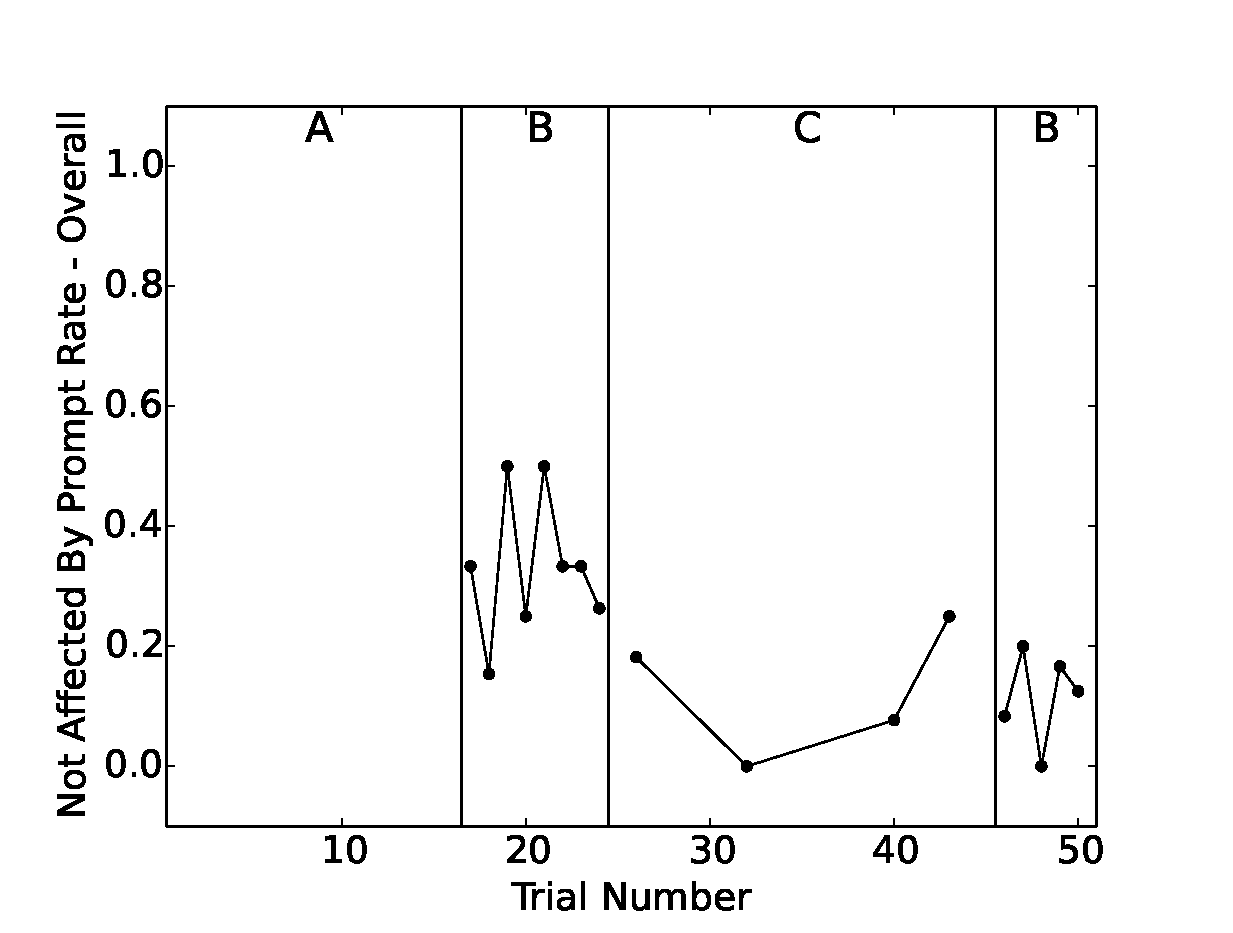
\includegraphics[width=0.6\textwidth]{./img/data_analysis/99NotAffectedByPromptRate-Overall_robotAloneOnly.eps}
	\caption{Not Affected By Prompt Rate - Robot Alone Trials}
	\label{fig:99NotAffectedByPromptRate-Overall_robotAloneOnly}
\end{figure}

As a summary of our primary results, we found that the robot was effective in guiding the child with ASD through hand-washing steps.  This was seen by a increased Number of Complete Steps and reduced Number of Parent Prompts as well as a maintained level of Prompt Compliance Rate.  Furthermore, we found that the child's compliance to robot prompts was not ideal when the robot was first introduced.  Through a training phase of the parent telling the child to follow the robot, the compliance rate was immediately improved.

\subsection{Secondary Results}
In addition to investigating the child's compliance in different intervention phases, we also attempted to characterize the child's engagement level, and possibly draw a causal link between higher engagement level and greater compliance.  We used measures Number of Times Child Smiles, Number of Times Child Murmurs, and Looking at Parent / Robot Rates (see Section \ref{sec:measures} for definitions) to characterize the child's engagement level during prompts and task executions.  However, we did not observe a correlation between any of these measures to the child's compliance rate.

The Number of Times Child Smiles did have a low level in First Phase B compared to Phase C and Second Phase B, but the level in Phase A should have been higher to be correlated with Compliance Rate.  Thus, although we can say the child tends to smile more in the later two phases, indicating that the child is more relaxed and having more fun, we can not draw a link between having fun and better compliance to prompts.

The Number of Times Child Murmurs did have a low level in First Phase B compared to Phase A and Phase C, but the level in Second Phase B should have been higher to be correlated with Compliance Rate.  What we found was that the child tends to murmur for two major reasons: in repeating the verbal prompt heard when the child is very engaged, and in protesting to the parent when the child does not wish to execute as prompted.  Thus, one could argue that this measure is not an ideal indicator for child's engagement level.  We also observed that the target to whom the child murmured to was often the parent, not the robot.  This may suggest that the child did not view the robot as a person one can communicate with, or that the child viewed the parent as the authoritative figure to appeal to in protest, not the robot.

The Looking at Robot Rate - Given Robot Prompted showed a high level in First Phase B, but decreased in the later two phases.  This is in contrary to the Compliance Rate, so no correlation was observed.  However, in comparison with Looking at Parent Rate and Given Both Prompted, we saw that the child prefers looking at the parent more than looking at the robot.  Also, the child looked at the robot more in the beginning of trials, but as trials went on, looked at the robot less.  This may be due to the robot not having a visually appealing appearance to the child.  The parent in Post-Intervention Survey also reported a lower level of satisfaction towards the robot's physical appearance.  Also, the appeal of the robot to the child may lie in not only its static appearance, but also the dynamics of its gestures and facial expressions.

\subsection{Limitations and Future Works}
Our Wizard of Oz study had many limitations.  The biggest one was having only one participant in the study.  This means our results maybe only applicable to this particular child, but not generalizable to the whole children with ASD population.  The next study in the future should increase the number of participants (maybe around ten subjects) while validating the major results of the current study.  The single subject research design should be used for this future study, since due to the diverseness of the children with ASD population, measures may have different levels across subjects.  Thus, we should generalize the effectiveness of an intervention by comparing the amount of change of measure levels for each child when having the intervention compared against him / her not having the intervention.  Also, the secondary aim of this future pilot study is to find out the participant demographics of a subpopulation of children with ASD that our intervention works consistently well on.  Only after this future study validating our major results and after we choose a subpopulation to focus on, should we attempt a larger scale (maybe around thirty subjects) randomized control trial, in which we divide the participants into control and intervention groups, and generalization of intervention effectiveness is made by directly comparing the measure levels between groups.  The focus of this randomized control would be to show clinical effectiveness of our intervention on the focused subpopulation.

Qualitative visual analysis was employed for the current study, where measure levels and trends were eyeballed.  We chose this analysis method due to its convenience, while accepting its inaccuracy as one of our limitations.  We felt that this inaccuracy is acceptable at the current stage of research -- having only one subject, with relatively few number of trials, and large noise in our measures.  However, as we move to the two future experiments mentioned above, quantitative analyses would be essential.  The pilot study could also employ visual analysis to make results comparable with the current study.  However, the randomized control trials study should strictly employ quantitative analysis only.

Another limitation was the reported change of robot control scheme in the middle of the First Phase B.  The reason for change was because our participant required a much more reactive robot who can switch the current step being prompted on the fly.  We felt the change was essential -- both the parent and the robot operator (the researcher) felt the robot was more responsive to the child after the control scheme switch.  However, the parent did report that the robot was still too slow for the child, and sometimes the pause between robot actions were too long.  We expected to see a change of measure levels due to robot scheme change.  However, due to noise in our measures, we could not observe such change.  Instead, only the change due to the parent robot training phase (Phase C) was apparent despite noise.  We felt the robot control scheme change was acceptable, since the focus of the current study is explore the possible questions and issues we might face In future experiments.  Thus, in future experiments we require the robot control scheme to be fixed.

Relating to the previous limitation was the fact that the current study (Wizard of Oz) involved a human operator (the researcher) remotely controlling the robot.  The researcher had no experience guiding the participant through hand-washing prior to the trials, and thus it was a learning process for the researcher through out the trials as well.  This meant that the researcher changed the order of steps the robot prompts were delivered to best fit the child's preference (e.g. the child preferred to put on soap before turning on water).  Also, the researcher chose prompts that were more effective (e.g. the attention grabber was not effective and so was not used in the end, and the child did not distinguish between scrub hands and rinse hands, so scrub hand prompts were not used in the end).  These changes were gradual, but may play a confounding effect on our measures.  However, we believe our major results, which reported an immediate change in Phase C, still stands despite the operator's learning effects.  One thing this does affect, though, is that in the future when we are automating the robot behaviors, tuning the robot prompts and order of steps to each child's preference is an inevitable task part of the automation process.

There are many sources of noise in the measures of the current study.  One of them is from the annotator(the researcher)'s subjectiveness when annotating the videos.  The annotator subjectivity may influence the different measures in varying degrees.  For example, when the parent repeats a verbal prompts several times in a roll, it is up to the annotator's discretion how many verbal prompts were issued.  Also, when the child executes a step almost simultaneously as a prompt is delivered, it is up to the annotator's discretion whether the prompt counts towards getting the child to execute the step.  Lastly, due to occasional obstruction of view and audio noise from running water, it is sometimes hard for annotator to tell whether the child smiles, murmurs, and looks at prompting parent / robot from the video.  All of the above are accepted as limitations of the current study, but can be improved through a more rigorous video annotation framework and better placement of video camera.  In addition, in future studies, the degree of annotator subjectiveness can be characterized by an inter-rater agreement measure such as the Cohen's Kappa \cite{volkmar2005handbook}.

Other confounding variables that produced measurement noise includes the following: First, the child was learning and getting better at hand-washing.  Although the child knew how to execute most of the hand-washing steps, he improved in remembering which step is next better through the trials, making him less and less dependent on prompts.  Second, the child's performance was influenced because he was new to the HomeLab washroom environment, which he gradually got used to the more he visited the lab.  The above two sources of noise can be reduced in future experiment through better control and maybe a per-trial training session to familiarize the child with the activity and the environment.  Thirdly, some measures were naturally noisy, due to the phenomenons they are measuring (e.g. the Number of Times Child Smiles or Murmurs could have been influenced by many factors unknown to the researcher).  Maybe better measures could have been chosen in the future.

One more limitation existed in our experiment protocol, specifically in regulating how the parent prompts in Phase C.  During Phase C, where the parent prompts the child alongside the robot, we gave the parent freedoms to decide how best to prompt.  Firstly, the parent could choose between verbal prompting in competition with the robot prompts, verbal prompting complementary to robot prompts, and physical prompting complementary to robot prompts [sec ref].  The parent decided to focus on the latter two, and alternated between the two as she saw fit.  Secondly, the parent could decide when to prompt relative to robot prompts.  In general, the parent prompted immediately after the robot.  However, there are cases where the parent prompts simultaneously with the robot, or even before the robot.  These uncontrolled variables of how the parent prompts in Phase C added noise on measures such as Number of Parent Prompts and Compliance Rate directly and other measures indirectly during this phase.  However, our major result, that Phase C acted as a training phase that resulted in effectiveness improvement of robot prompts, still holds.  What it does affect, though, is that we do not know which variable regarding how the parent prompts in Phase C was most beneficial in improving robot prompt effectiveness.  Thus, in future experiments, controlling how the parent prompts in the training phase is needed to better understand how to consistently improve robot prompt effectiveness.

Lastly, there is a limitation due to the experiment environment.  The current study was carried out in the HomeLab washroom in the Toronto Rehab hospital.  This lab setting is not ideal, in contrast to conducting the experiment in the home settings, in that: it is not an environment the child is familiar with (as mentioned in previous paragraph already); also, it requires the child to wash hands many times in a roll as opposed to only wash hands before meal and after toileting, creating fatigue and lacking real motivation.  We chose the HomeLab instead of home settings for this study because the Wizard of Oz study requires the researcher to operate the robot and monitor the child remotely (out of the child's view), which is hard to implement in the home settings.  For future experiments, especially the randomized control trials study, can venture in carrying out the experiment in the home settings, with the robot behavior fully automated.  Careful planning and parent educating of the parent prompting protocol during Phase C is needed to produce meaningful results.

In our study, we've established the link between compliance rate and prompt effectiveness.  Furthermore, we've shown that the initial compliance rate to robot NAO was low, but can be improved through a training phase with the parent.  Thus, for future experiments, instead of examining the training phase, we could also focus on investigating how to improve the initial compliance rate through better robot appearance and behavior designs.  For one, we can investigate if changing the robot appearance from humanoid to animal helps improve compliance.  Secondly, the verbal reward can be changed to fun animal or cartoon sounds, and task execution can be made more fun by playing back a cartoon tune of choice from the robot.  LED lights on the robot may be another mean to make the robot more salient to the child.  When investigating the effects of these design changes, it is essential to establish secondary measures besides compliance rate and prompt effectiveness.  More thoughts and literature research should be given in the future studies for choosing measures for measuring child engagement.  Lastly, we can investigate the impact of embodiment by comparing a physical robot with its virtual avatar (a video recorded version of the robot displayed on the monitor).  If they show similar effectiveness, it would potentially cut down the cost of the intervention by a significant amount, making the soluion commercially available immediately.  Also, this comparison may yield key clues in why the parent is currently a better prompting agent than the robot -- maybe the parent exerts a more authoritative presence than the robot, and the robot than its virtual avatar.

Finally, here are some suggestions for improvements from the parent in the Post-Intervention Survey that are not mentioned in previous sections:  The robot can improve its pointing better so that the child sees exactly which object he needs to interact with.  This can be done by having more fingers on the robot's hands, or by attaching a light source (e.g. laser pointer or mini-projector) that the robot can use to highlight physical objects at the sink.  The robot would be more visible if it is bigger or placed at eye level of the child.  It would be ideal if the robot is mobile, and can prompt other activities of daily living besides hand-washing.  Lastly, attaching permanent cameras in the washroom is not okay, since the child is not the only one using the washroom.  Thus, having a mobile robot that follows the child would be a better solution.

\chapter{Visual Focus of Attention Estimation}
From the WoZ pilot study, we have learned that the participant did not look at the robot as often as he did at the parent.  This means that the robot and its actions were not visually stimulating enough to motivate the participant to focus his attention upon.  Although no correlations between VFOA on robot and Compliance Rate was observed for our participant, literatures suggest that keeping the child with ASD visually engaged during action modeling when teaching a new skill is essential [\ref{Sec:AT4ASDDiscussion}].  Thus, it is helpful to be able to track the VFOA of the child with ASD during the hand-washing activity, so that the robot actions may adjust automatically to better engage the child's visual attention.

To track the VFOA of the child, we are using the Microsoft Kinect to collect RGB and depth images of the child's head.  Gaze directions can be tracked more accurately when head is viewed near frontal, and since we cared more about the child's attention to prompting agents than to sink objects, we setup the Kinect near the robot, and have sink objects further from the Kinect (i.e. soap and towel) be spread apart from each other to be easily distinguished.

The problem of estimating the object under child's attentional focus is broken into three parts: head pose estimation, eye pose estimation, and object identification.


%Overall objective
%	- to implement a real time gaze tracker
%a short reason why, so we know what's good enough and what's important to focus on
%
%2D webcam Approach:
%	- BLAH face tracker, eye corner extraction, stretch based inverse pose transformation, evaluation
%	
%	
%3D Kinect camera approach:
%	- KinFu mesh building, ICP head pose tracking, point cloud based inverse transformation, evaluation
%	- challenges of children with ASD footage, future algorithm requirement



\section{Head Pose Estimation}

%\subsection{2D Video Camera Approach}


%http://face.ci2cv.net/
%https://github.com/ci2cv/face-analysis-sdk
%http://face.ci2cv.net/doc/





\subsection{3D Kinect Camera Approach}

\subsubsection{Approach Overview}
\label{sec:approachOverview}
An accurate way for gaze tracking is to use the Kinect depth sensing camera so that we track the head pose using 3D data.  The idea is to first build a 3D model of the specific user's head using several frames of the depth images.  Then we can fit the model through rigid transformation onto new frames of depth video stream to estimate the head pose in real-time.  After the head pose is obtained for a depth frame, we transform the corresponding frame of color image to the frontal head pose, and crop out the eye regions for gaze prediction.  This method is more accurate than any 2D non-transforming method for the following reasons.  First, the color image is transformed into a frontal pose, and this transformation introduces minimal distortion to the image given the tracking is good, and makes the eye pose detection much easier and more accurate.  Second, when cropping the eye regions from the color image, we can specify the eye cropping regions ahead of time.  Since all color images are now in frontal pose, the cropping regions remain the same even when the user is rotating his/her head.  This gives a more accurate and more stable cropping.  Of course, the two advantages for this method are both dependent on that the head pose tracking is accurate.

\subsubsection{KinFu Head Modeling}
%what are we trying to achieve
%why do it this way
%open source kinfu, how it works
%what I did to fit it to our purpose
%results achieved
We would like to choose a method for building a user specific 3D model of the head that requires minimal user interactions.  This is because we are focusing on the children with ASD population.  Asking a child with ASD to sit still and keep head straight for a period of time for a 3D laser scanner to scan his/her head is less feasible.  Instead, we aimed to obtain the head model through a short video stream of the Kinect's depth frames captured as the child came into the washroom and stood in front of the sink, without trying to restrict the child's movements.

To achieve this, two pieces of softwares are essential.  One is Point Cloud Library (PCL)'s KinFu, which enables us to integrate the frames from Kinect's depth video stream into a single 3D model of the scene.  The second software is Microsoft Kinect for Windows (K4W) SDK's Skeleton Tracking, which enables us to track where the user's head is, and so that only the head is reconstructed by KinFu.

\paragraph{How KinFu Works}
PCL is an open source stand alone library that processes 3D data in the form of point clouds (collections of 3D points).  It provides functionalities such as filtering, normal estimation, feature extraction, transformations, segmentations, surface reconstructions, etc \cite{rusu20113d}.  KinFu is PCL's open source implementation of Kinect Fusion \cite{pirovano2011kinfu}, an algorithm first proposed by Microsoft and demonstrated in its KinectFusion API in K4W SDK \cite{newcombe2011kinectfusion}.  The idea of Kinect Fusion is related to the traditional Simultaneous Localization And Mapping (SLAM) algorithm \cite{pirovano2011kinfu}, where feature points in the scene are matched across frames of a 2D video stream, so that the camera's orientation within the scene is tracked across frames.  At the same time, the frames are patched together to build a sparse 3D map of the scene.  Kinect Fusion extends SLAM into a dense version where every point in the point cloud now becomes a feature point and the full 3D scene is reconstructed \cite{newcombe2011kinectfusion}. It also makes usage of the General Purposed GPU (GPGPU)'s parallel computation to speed up the algorithm to real-time.  The PCL's KinFu and Microsoft's KinectFusion implementations have similar processing pipeline -- they only differ in some specific low level algorithms used.  Below is KinFu's processing pipeline \cite{newcombe2011kinectfusion}:

\subparagraph{Preprocessing}
First, the depth frame from the Kinect camera is filtered through bilateral filtering to remove noise -- it selectively smooths the surfaces while preserving edges \cite{tomasi1998bilateral}.  The bilateral algorithm's effect is illustrated by Figure \ref{fig:bilateralFiltering}.
\begin{figure} [h]
	\centering
	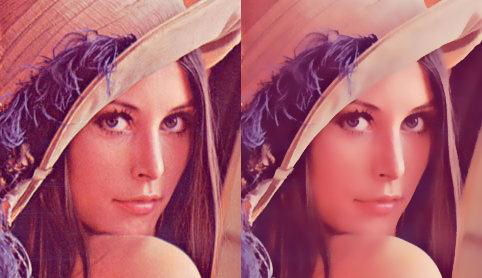
\includegraphics[width=0.6\textwidth]{./img/bilateral_filtering.jpg}
	\caption{A bilateral filter applied to a 2D color image.  The left is the original, while the right is filtered, resulting in removal of noise, figure adapted from \cite{pirovano2011kinfu}}.
	\label{fig:bilateralFiltering}
\end{figure}

If at time \(k\), the raw depth map \( R_k \) gives a depth measurement \( R_k(\textbf{u}) \) at image pixel \( \textbf{u} = (u,v)^T \) in the image domain \( \textbf{u} \in U \), then the bilateral filtered depth map \( D_k \) is given by:
\[  D_k(\textbf{u}) = \frac{1}{W_p} \sum_{\textbf{q} \in U}^{} \mathcal{N}_{\sigma_s}(\| \textbf{u} - \textbf{q} \|_2)  \mathcal{N}_{\sigma_r}(\| R_k(\textbf{u}) - R_k(\textbf{q}) \|_2) R_k(\textbf{q})  \]
, where 
\[ \mathcal{N}_{\sigma}(t) = exp(-t^2 \sigma^{-2}) \]
, and a normalizing constant 
\[  W_p = \sum_{\textbf{q} \in U}^{} \mathcal{N}_{\sigma_s}(\| \textbf{u} - \textbf{q} \|_2)  \mathcal{N}_{\sigma_r}(\| R_k(\textbf{u}) - R_k(\textbf{q}) \|_2)  \] 

After filtering, multiple resolutions of the depth frame is generated through sub-sampling, we call them the multi-resolution pyramid, illustrated by Figure \ref{fig:resolutionPyramid}.  Lastly, each layer of the pyramid generates a 3D point cloud through back projection using the camera's calibration matrix, \(\textbf{K}\), obtaining the point cloud (or vertex map) \(\textbf{V}_k\) in world coordinate,
\[  \textbf{V}_k(\textbf{u}) = D_k(\textbf{u}) \textbf{K}^{-1} \dot{\textbf{u}} \]
, where \( \dot{\textbf{u}} := (\textbf{u}^T|1)^T \)
\begin{figure} [h]
	\centering
	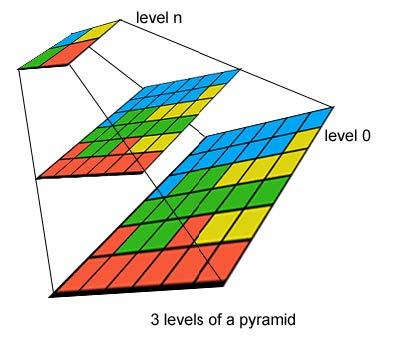
\includegraphics[width=0.6\textwidth]{./img/resolution_pyramid.jpg}
	\caption{A 3-level multi-resolution pyramid, figure adapted from \cite{pirovano2011kinfu}}.
	\label{fig:resolutionPyramid}
\end{figure}

In each point cloud, the normal for each point is estimated by an eigenvector of Principal Component Analysis (PCA) of its neighborhood points \cite{pirovano2011kinfu}.


\subparagraph{Alignment}
The preprocessed point clouds now need to be aligned to the current scene model.  If this is the very first depth frame, then its point cloud is used as the current model -- alignment starts at the second frame.  Alignment is done through the Iterative Closest Point (ICP) algorithm (with some modification of its procedures), starting from the point cloud of the coarsest layer in the pyramid.  ICP is performed in loops until one of the exit criteria is met, after which the same is done for the point cloud of the next level in the pyramid, and the next, until all levels are traversed.

The ICP loop (the modified version) has the following procedures:  Both points from the new frame's point cloud and the model's point cloud are projected to the model point cloud's camera image frame, and any pair of points from the two clouds falling onto the same pixel is noted as a match.  Then the rigid transform that globally minimizes the sum of squared errors between matched points is calculated, the error being the distance between the point of new cloud to the tangent plane of point of the model cloud, seen in Figure \ref{fig:pointToPlaneError} \cite{low2004linear}.
\begin{figure} [h]
	\centering
	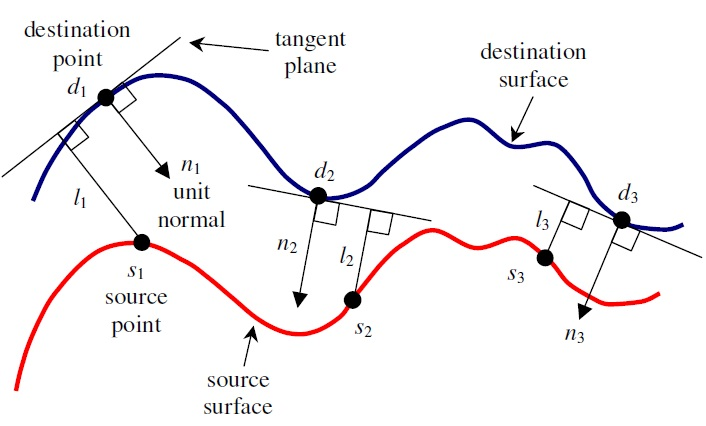
\includegraphics[width=0.6\textwidth]{./img/point_to_plane_error.jpg}
	\caption{Point-to-plane error between two surfaces, figure adapted from \cite{low2004linear}}.
	\label{fig:pointToPlaneError}
\end{figure}


If for a pair of points, \( \textbf{s}_i = (s_{ix}, s_{iy}, s_{iz}, 1)^T \) is the source point, \( \textbf{d}_i = (d_{ix}, d_{iy}, d_{iz}, 1)^T \) is the matched destination point, and \( \textbf{n}_i = (n_{ix}, n_{iy}, n_{iz}, 0)^T \) is the unit normal vector at \( \textbf{d}_i \), then in each ICP loop, the rigid-body transformation matrix \( \textbf{M} \) is found by
\[  \textbf{M}_{opt} = arg min_\textbf{M} \sum_{i}^{} ((\textbf{M} \cdot \textbf{s}_i - \textbf{d}_i) \cdot \textbf{n}_i)^2  \]

The exit criteria for the ICP loop are either 1) the maximum number of iterations are reached, 2) the changes of the transformation matrix falls below threshold, or 3) the sum of squared errors fall below threshold.

\subparagraph{Surface Reconstruction}
Finally, the aligned new frame needs to be integrated into the model and to form a new model point cloud so the pipeline can loop from the top as frames arrive.  A new model point cloud is formed by first converting the two clouds into Truncated Signed Distance Functions (TSDF).  A TSDF is basically a representation of surfaces of objects in a scene, with negative values assigned to voxels inside the surface or voxels that are not measured yet, positive values assigned to voxels outside the surface, increasing in value as we move further away from the surface, and voxels on the surface of objects are assigned the value of zero, illustrated in Figure \ref{fig:TSDF} \cite{newcombe2011kinectfusion}.  Here the raw value of the new frame with no filtering is used for calculating its TSDF to avoid losing details.
\begin{figure} [h]
	\centering
	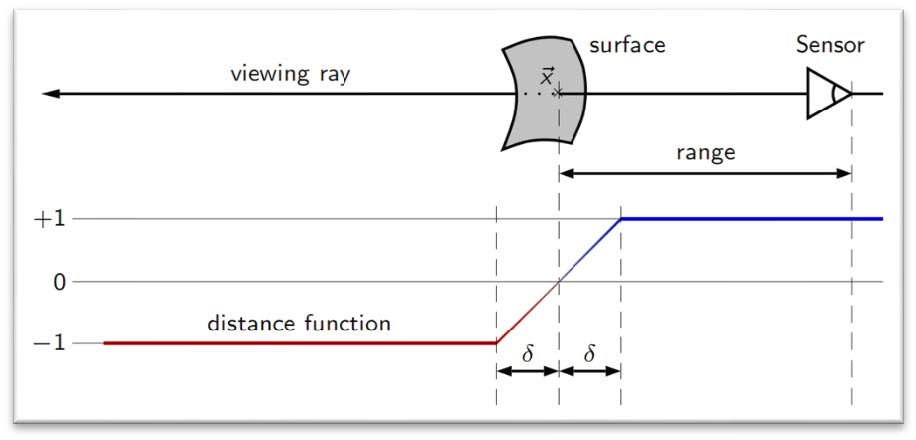
\includegraphics[width=0.6\textwidth]{./img/TSDF.jpg}
	\caption{A illustration of creating an 1D TSDF, figure adapted from \cite{pirovano2011kinfu}}.
	\label{fig:TSDF}
\end{figure}

Specifically, at a point \(\textbf{p}\) in the world coordinate, its projected nearest pixel \(\textbf{x}\) in the depth frame is given by,
\[  \textbf{x} = \lfloor \pi (\textbf{K} \textbf{M}^{-1}_{k} \textbf{p}) \rfloor  \]
, where \( \lfloor.\rfloor \) is the nearest neighbor lookup, and \( \textbf{q} = \pi(\textbf{p}) \) performs perspective projection of \(\textbf{p} = (x,y,z)^T\) with dehomogenization to obtain \(\textbf{q} = (x/z, y/z)^T\).

The TSDF \(F_{R_k}\) of a depth frame \(R_k\) at point \(\textbf{p}\) is computed as,
\[  F_{R_k}(\textbf{p}) = \Psi(\lambda^{-1}\|\textbf{t}_k - \textbf{p}\|_2 - R_k(\textbf{x}))  \]
, \[  \lambda = \|\textbf{K}^{-1} \dot{\textbf{x}} \|_2   \]
, 
\[
\Psi(\zeta) = 
\begin{cases}
min(1, \frac{\zeta}{\mu}) sgn(\zeta)  & \text{iff}\ \zeta \geq -\mu \\
\text{null} & \text{otherwise}
\end{cases}
\]
, where \(\textbf{t}\) is the translation part of the rigid body transformation matrix,
\[  \textbf{M} = 
\begin{bmatrix}
\textbf{R}		&	\textbf{t} \\
\textbf{0}^T	&	1
\end{bmatrix}  \]
, and \(\lambda^{-1}\) converts ray distance from frame origin to \(\textbf{p}\) to a depth value, and \(\Psi(.)\) truncates the SDF to a tolerance \(\mu\) within which distance to the uncertain depth measurement we expect the true value to lie.

After obtaining the TSDFs of the two clouds, volume integration of the two clouds are achieved by a weighted running average of the model cloud's TSDF with the new frame cloud's TSDF.
If the model before integration has TSDF \(F_{k-1}\), then integrating the new frame's TSDF \(F_{R_k}\) gives
\[  F_k(\textbf{p}) = \frac{W_{k-1}(\textbf{p}) F_{k-1}(\textbf{p}) + W_{R_k}(\textbf{p}) F_{R_k}(\textbf{p})} {W_k(\textbf{p})}   \]
\[  W_k(\textbf{p}) = W_{k-1}(\textbf{p}) + W_{R_k}(\textbf{p})  \]
, where \( W_{R_k}(\textbf{p}) \)is the weight used for correcting noisy measurements due to distance from sensor center, and is proportional to \( cos(\theta)/R_k(\textbf{x}) \), \(\theta\) the angle between the direction of the associated pixel ray and the surface normal.

Lastly, surface reconstruction is done through the marching cube algorithm, which converts the new model's TSDF into a point cloud.


%http://research.microsoft.com/pubs/155378/ismar2011.pdf
%http://homes.di.unimi.it/~pirovano/pdf/3d-scanning-pcl.pdf
%http://pointclouds.org/documentation/tutorials/normal_estimation.php

%- KinFu
%	- noise removal via bilateral filtering
%	- creation of multi-resolution pyramid (through sub-sampling)
%	- forming 3D point cloud (through back projection using cameras' calibration matrix) and normal estimation (through eigenvalue estimation) for each layer
%	- alignment (through ICP)
%		- for each point, search, within predefined radius, for its closest point
%		- calculate the rigid transform that minimizes sum of squared distances of all point pairs
%		- repeat this process until
%			- maximum number of iterations reached
%			- difference in transformations fall below threshold
%			- sum of squared distances fall below threshold
%		- KinFu makes modification:
%			- assumes small difference between frames!
%			- in order to parallelize computation, instead of searching for closest point in 3D space, it projects the two clouds onto the first cloud's camera image frame (2D), and pair all points that fall onto the same pixels.
%			- loops through ICP algorithm starting with coarser point clouds first, and works its way down the pyramid
%			- uses point to plane distance metrics instead of point to point, converging faster		
%	- surface reconstruction (through TSDF (Truncated Signed Distance Function) volume integration and marching cube surface reconstruction)
%		- raw depth data is used for merging into model instead of the filtered ones to avoid losing details
%		- calculate TSDF of current model and the new cloud to be merged
%		- merge the two TSDFs using weighted running average
%		- marching cube for reconstructing surface of the updated model's TSDF, creating a smoother point cloud with normals for registering next frame using ICP

\paragraph{Using KinFu with Kinect2 Camera}
To use KinFu with Kinect2 Camera, the open source PCL Kinect2 SDK and PCL Kinect2 KinFu by Steven Hickson (available on GitHub.com) are used.  They act as a driver for Kinect2 camera using the PCL point cloud framework.  This SDK currently only supports generating 3D non-color point cloud from the depth frames of Kinect2.  We had to implement the generation of color point cloud using the color frames ourselves.  However, the advantage of using this over using Microsoft Kinect2 for Windows SDK is that: first, Kinect Fusion was only in an unstable beta version in the Windows SDK during the time this thesis was conducted; second, the open source nature of PCL's KinFu enables us to have much more control in using the algorithm for our application.  The modifications to the KinFu algorithm are outlined in the sections following.


\paragraph{Using KinFu for Head Modeling}
Using KinFu for head modeling is very similar to the original purpose of KinFu -- scene modeling.  The difference lies that, for object (e.g. a head) modeling, we need to filter everything except the object of interest in the depth frame, so that KinFu only builds the 3D model over data on the object, and ignores everything.  One thing that's neat about object modeling is, instead of rotating the Kinect camera around the object, we can rotate the object while fixing the camera.  Also, specifically for head modeling, we can utilize Kinect's Skeleton Tracking algorithm to filter out everything except the head.

Not all objects can be tracked using the ICP algorithm in KinFu.  In KinFu's paper, the author reports that whenever the object is moving too quickly or when not enough 3D features (e.g. edges and corners) are present on the object surface, ICP often fails \cite{pirovano2011kinfu}.  This is mainly due to the assumption in ICP that between frame movements are small (note that this problem may be potentially solved by higher frame rate camera with higher computational power so no frames are skipped).  However, for head tracking, KinFu turns out to work just fine as long as the person isn't moving his/her head too fast.  Shown in Figure \ref{fig:headTrackingResults} (b) is an example 3D mesh model created using the above method.
\begin{figure} [h]
	\centering
	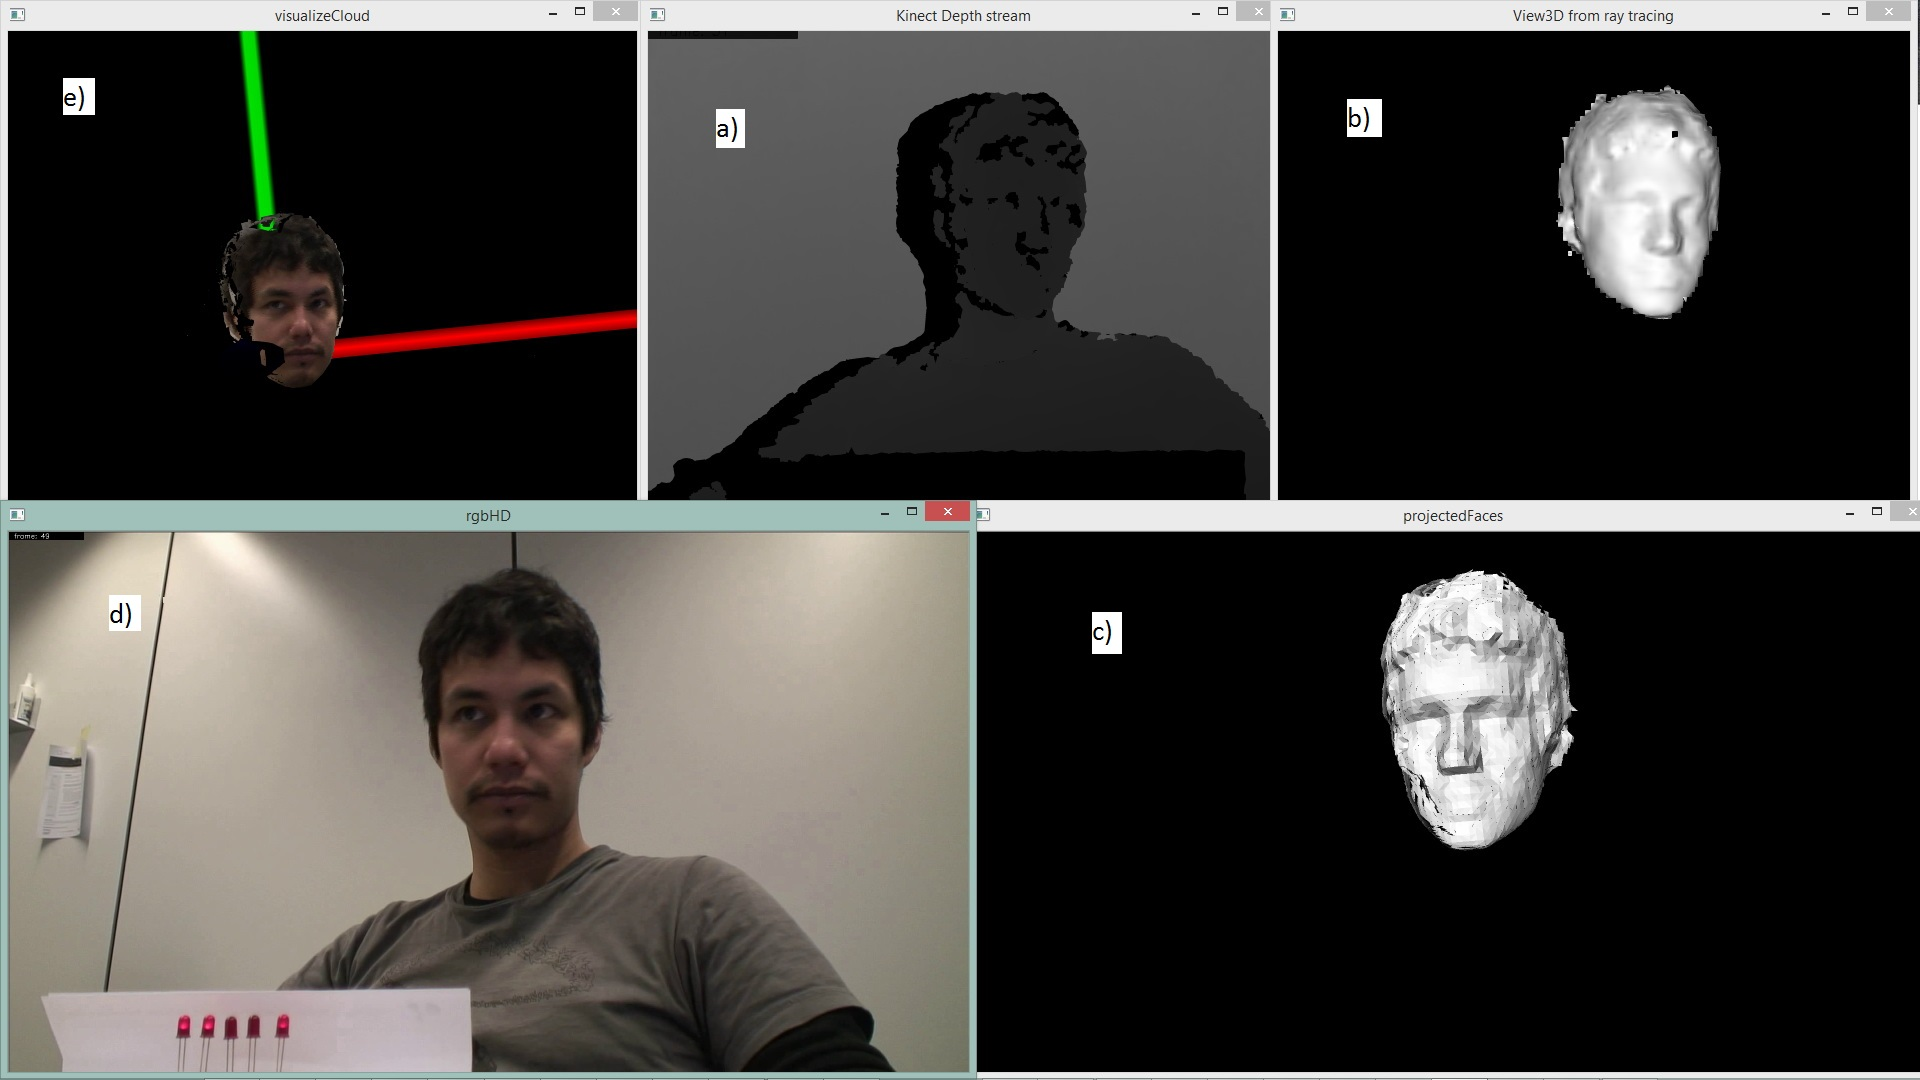
\includegraphics[width=\textwidth]{./img/headTrackingResults1.jpg}
	\caption{The 3D Kinect Camera Approach Results: we start by grabbing a frame from the Kinect depth camera (a), then we fit the 3D head model to the depth frame (b), after which we project the head model mesh onto the color camera image plane (c), so as to associate the color pixels with the head model mesh (d), and lastly forming the 3D color point cloud (e).}
	\label{fig:headTrackingResults}
\end{figure}

Also, facial expressions deform the face, making it deviate from the learned head model, and tracking accuracy may suffer due to the ICP's rigid nature.  Thus we see that the robustness of ICP head tracking depends on two factors:
\begin{itemize}
	\item the head's movement speed (both translational and rotational) relative to the ICP loop process speed or the Kinect camera's frame rate (which ever is the bottleneck)
	\item the dynamics of facial expressions on the head
\end{itemize}

An evaluation of KinFu's capability for head modeling can be done by finding the maximum movement speed of the head (both translational and rotational) under expressionless vs. moving jaw faces conditions before KinFu's alignment step fails.  However, due to limitation of time, the algorithm's capability was not evaluated.


\subsubsection{KinFu Head Pose Tracking}
After obtaining the user's 3D head model, the 3D position and pose (pitch, yaw, and roll) of the head can be tracked in the depth video stream using KinFu.  Skeleton Tracking is again used to filter out everything except the head in the depth video stream.  In addition, it is used to give initial position of head for the ICP loop, so that new frames to be aligned are within the capability of ICP.  Also, the KinFu algorithm needs to be modified to skip the surface reconstruction step, since we already have a model of the head.

A similar evaluation of algorithm capability as mentioned above for KinFu head modeling can be done to see KinFu's robustness in head tracking.  However, this was not conducted due to time limitations.


\subsubsection{Point Cloud Based Inverse Pose Transformation}
Having accurate head model and head pose tracking enable us to restore the color image frames of the user's head into frontal pose.  This inverse pose transformation is done by first forming a colored point cloud from the color frame, then 3D rigid transforming the point cloud inversely to the head pose so that the head represented by the point cloud is in frontal pose, finally projecting the transformed point cloud onto the camera image plane to obtain the 2D color image of the frontal posed head.

\paragraph{Colored Point Cloud}
To form a colored point cloud, we need to calculate the 3D coordinates of every pixel in the color frame.

The function "MapColorFrameToCameraSpace" provided by K4W SDK is for this purpose, and is used by the PCL Kinect2 KinFu SDK by Steven Hickson.  However, MapColorFrameToCameraSpace provides the 3D coordinates of color pixels by associating each pixel in the color frame with a pixel in the depth frame, and then calculating the 3D coordinates of every pixel in the depth frame.  This approach is convenient to code and fast in execution, but is limited by the depth frame resolution.  For the typical resolution of the Kinect2 camera, the color frame resolution is 1920 X 1080 (2073600 pixels), the depth frame resolution is 512 X 424 (217088 pixels).  Using the above method, 2073600 pixels are available in color frame, but can only form 217088 unique points in the point cloud.  This is an order of magnitude reduction, wasting the HD color frame provided by the Kinect2 camera.  For Kinect1 camera, with color frame and depth resolutions being 640 X 480 (307200 pixels), this is also a huge reduction in resolution.  This problem of using the depth frame resolution for point cloud greatly reduces the resolution of the resulting frontal pose color image, making the next step, gaze prediction, less accurate if not much harder.

To avoid resolution reduction, we use the 3D head model instead of the depth frame for calculating the 3D coordinates of each color pixel:

\subparagraph{Head Model Mesh Projection}
To do this, we first generate a triangular mesh version of the 3D head model.  Then we transform the head model mesh to match the pose in the current depth frame (done in previous step).  Next, we project the mesh onto the color camera image plane, keeping track of which pixel each vertex of the mesh lands on.  This enables us to mark which mesh surface each pixel in the projected image belongs to.  More specifically, for each mesh surface in the model, we do a depth first search traverse on the projected image starting with the pixel that one of the surface vertices projects to.  During traverse, we go to the pixel's neighbors one by one (there are eight adjacent neighbors to each pixel) if the pixel itself lies within the projected surface (i.e. inside the triangle formed by the surface's three projected vertices), and stop traversing if the pixel is outside of the projected surface, outside of the image boundary , or is already visited by the traverse.  There are times where two surfaces overlap in their projections -- this happens when one surface obstructs the view of the other (from the camera's point of view).  We handle this by assigning pixels to belong to the mesh surface nearest to the camera's focal point.  The result of this head model mesh projection is shown in Figure \ref{fig:headTrackingResults} (c).

\subparagraph{3D Coordinate Calculation}
After assigning surfaces to every pixel, the pixels' 3D coordinates can be calculated by linearly interpolating from the surface vertices.  To do this, we take advantage of the fact that Barycentric coordinates are preserved during projection of a planar object in 3D onto another plane.  Thus, a point on the 3D mesh surface preserves its Barycentric coordinate after projecting onto the color image plane.  Note that expressing a point in Barycentric coordinates w.r.t. a triangle it is on is basically expressing the point as a linear combination of two of the triangle's edges.  Mathematically, this means the following: Given triangular mesh surface vertices with coordinates P1, P2 and P3 in 3D, projected vertices with coordinates p1, p2 and p3 in 2D, and a point on the mesh surface with coordinate P in 3D, and projected coordinate p in 2D.  The Barycentric coorindate for P w.r.t. {P1, P2, P3} is \( (\lambda1, \lambda2, \lambda3)  \), with \( P = \lambda1 \times P1 + \lambda2 \times P2 + \lambda3 \times P3 \), \( \lambda1 + \lambda2 + \lambda3 = 1 \), and \( \lambda1, \lambda2, \lambda3 > 0 \).  Then, the Barycentric coorindate for the projected point, p, w.r.t. {p1, p2, p3} is also \( (\lambda1, \lambda2, \lambda3)  \), with \( p = \lambda1 \times p1 + \lambda2 \times p2 + \lambda3 \times p3 \).  Using this fact, we can calculate the Barycentric coordinate for each pixel w.r.t. the mesh surface it belongs to, and then calculate the pixel's back projected 3D coordinate using the surface's vertices' 3D coordinates.  An example of a colored point cloud formed using this method is shown in Figure \ref{fig:headTrackingResults} (e).

\paragraph{Inverse Pose Transformation}
With the color point cloud created, we are ready to form a frontal pose color image.  First, we rigid transform the cloud so that the center of the head is at coordinate (0, 0, 2 \( \times\) focal length) and its pose facing the origin.  The reason for 2 \( \times\) focal length is that the image plane is at 1 \( \times\) focal length, and we want the cloud to be a little distance away from the image plane so that the projection looks good inside the image boundaries.  Note that focal length is a programmer defined value used in the next step for perspective projection, and is the distance from image plane to the camera's focal point.

\subsubsection{Projection onto Camera Image Plane}
The last step before obtaining the frontal pose color image is the perspective projection.  For this, we go through every point in the color point cloud and calculate each point's 2D image coordinate.  If two points land in the same pixel, the one closer to the camera's focal point is used.  Several images of inverse pose transformed color point clouds projected onto the camera image plane are shown in Figure \ref{fig:inversePoseResults}.  We see that for moderate range of head poses, the algorithm works great.  However, at extreme range of head poses, distortions of the image and occlusions occur.  The distortion is mainly caused by the inaccuracy in head pose tracking as well as the crudeness of the 3D mesh head model (triangular mesh needs to be quite dense to approximate certain fine curves on the face, e.g. near the eyes).  The occlusion is a natural artifact due to lack of data from the RGB image.
\begin{figure}[h]
	\centering
	\begin{subfigure}[b]{0.32\textwidth}
		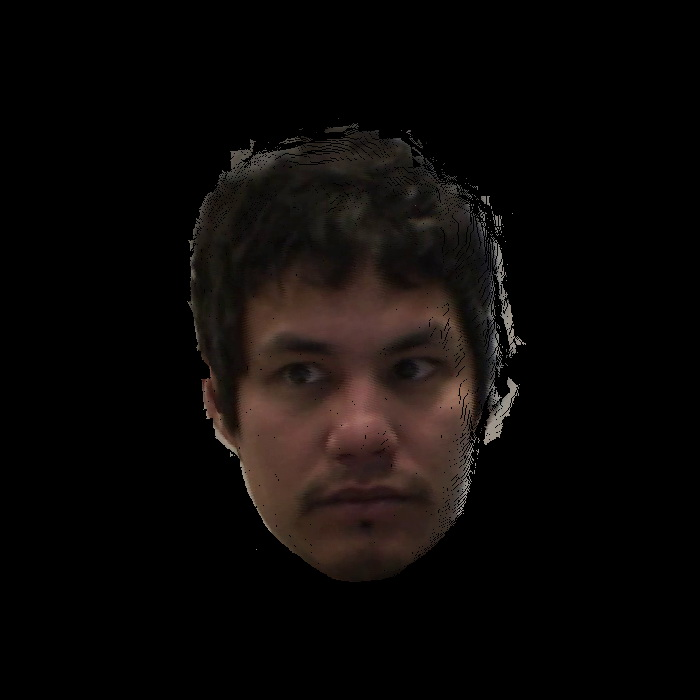
\includegraphics[width=1.1\linewidth]{./img/eyeimages/s1.jpg}
	\end{subfigure}
	\begin{subfigure}[b]{0.32\textwidth}
		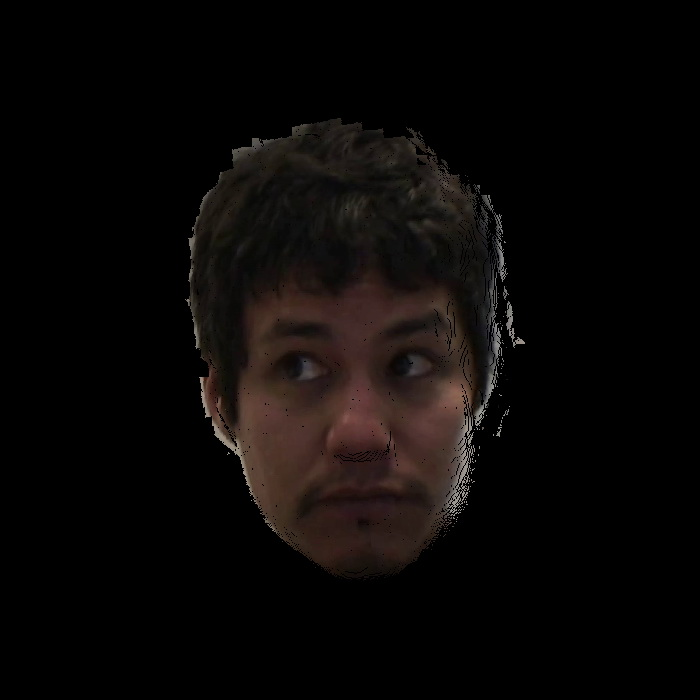
\includegraphics[width=1.1\linewidth]{./img/eyeimages/s2.jpg}
	\end{subfigure}
	\begin{subfigure}[b]{0.32\textwidth}
		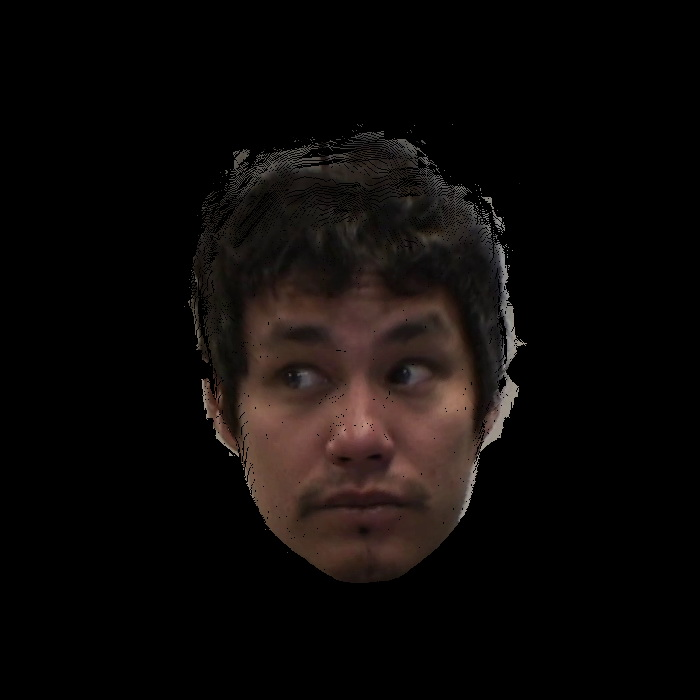
\includegraphics[width=1.1\linewidth]{./img/eyeimages/s3.jpg}
	\end{subfigure}
	\\
	\begin{subfigure}[b]{0.24\textwidth}
		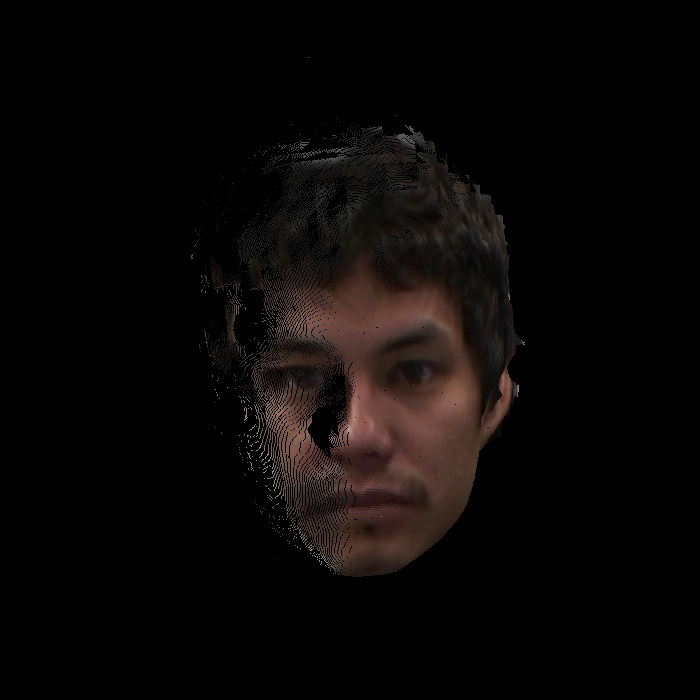
\includegraphics[width=1.1\linewidth]{./img/eyeimages/f1.jpg}
	\end{subfigure}
	\begin{subfigure}[b]{0.24\textwidth}
		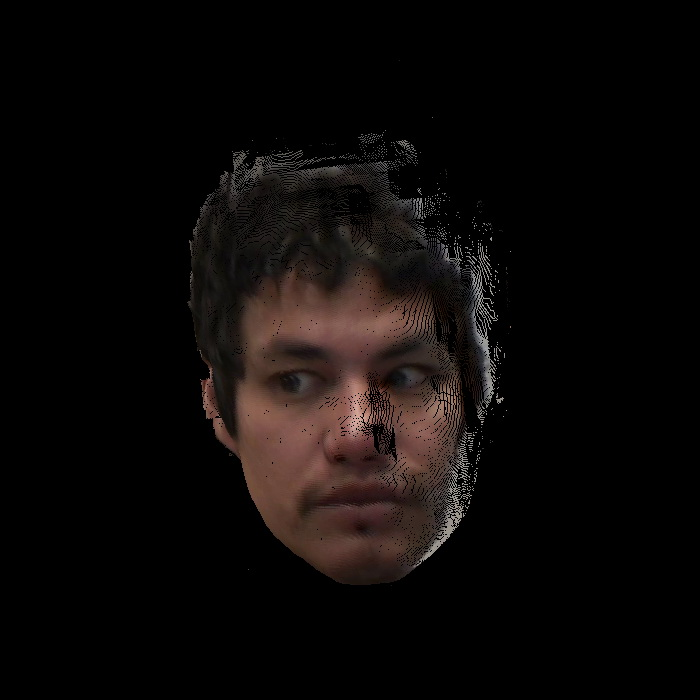
\includegraphics[width=1.1\linewidth]{./img/eyeimages/f2.jpg}
	\end{subfigure}
	\begin{subfigure}[b]{0.24\textwidth}
		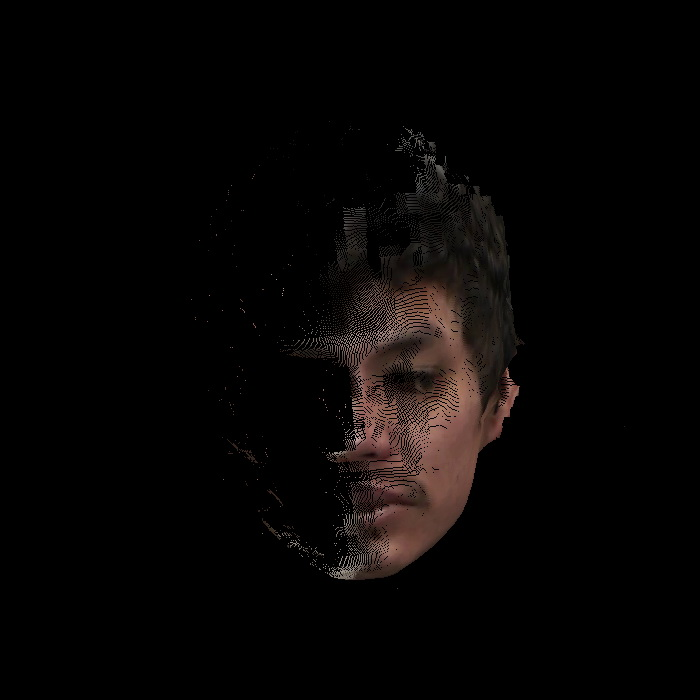
\includegraphics[width=1.1\linewidth]{./img/eyeimages/f3.jpg}
	\end{subfigure}
	\begin{subfigure}[b]{0.24\textwidth}
		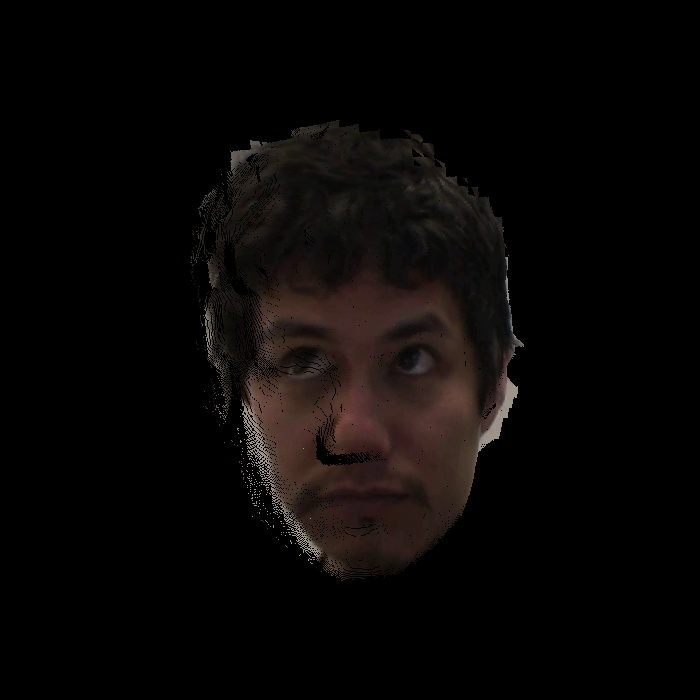
\includegraphics[width=1.1\linewidth]{./img/eyeimages/trackingError.jpg}
	\end{subfigure}
	\caption{Inverse Pose Transformed Color Images of an Example Head: The top row displays images of the head for moderate range of poses, showing little distortion and blank spots; the bottom row displays failure cases, the first three shows extreme head poses resulting in some distortions and huge blank spots due to occlusion, the last image shows a failure case due to head tracking error, resulting in large distortions.}
	\label{fig:inversePoseResults}
\end{figure}


There are pixels in the image that are blank because no points in the color point cloud landed on them.  When the cause of the blank spots is the point cloud being sparse, then the resulting projected image has scattered and small blank spots.  To this end, OpenCV's In-Painting algorithm is used to fill them \cite{bertalmio2000image}.  However, if the blank spots are caused by occlusion due to head pose, the spots are larger and more concentrated, and the In-Painting algorithm may be doing a poor job.  This only happens at the eye regions at extreme head poses, where other sources of distortion errors (e.g. head pose tracking inaccuracy) dominate.  Thus In-Painting being inaccurate in this case is tolerable, and treated as a limitation.

\subsubsection{Using the EYEDIAP Dataset}
Our ultimate goal is to predict the user's gaze given the depth and color video streams from Kinect.  So far, we are able to extract a frontal pose corrected color images of the eye regions.  The next step is to train a gaze predictor so the gaze direction can be predicted given a pair of eye region images.  To this end, we obtained the EYEDIAP Dataset \cite{mora2014eyediap}.

The EYEDIAP Dataset was created by the IDIAP Research Institute for the purpose of training and evaluating gaze prediction algorithms using depth and color video streams.  It consists of 16 participants, 12 males and 4 females.  Participants are asked to gaze follow visual targets while being recorded by a Kinect1 camera and a HD video camera.  For each participant, three visual target conditions are recorded: target on a computer screen changing positions discretely, target on a computer screen changing positions continuously, and a small moving ball floated by a long pole moving continuously.  For each condition, two sessions are recorded, with one requiring the participant's head to remain still while the other allowing free movement.  The videos are annotated automatically for head pose and gaze direction.  This is done by using the 3D Morphable Model (3DMM) algorithm for head tracking, knowing the location of the visual targets on screen, and extracting the location of the floating ball target from the depth data.  Using the annotations, gaze predictors can be trained and evaluated.

To use the EYEDIAP Dataset in our framework, further modifications to the KinFu algorithm were made.  First, instead of subscribing to the video sources of a Kinect camera, the depth and color videos of the dataset are read frame by frame using OpenCV.  Note that we are not using the Kinect1 camera's color videos; instead, the higher resolution HD camera videos are used along with the Kinect1's depth videos.  Depth frames are undistorted using the distortion calibration values provided, following the method used in the open source calibration toolbox by \cite{herrera2012joint}.  Also, image buffers' sizes are changed to match the HD video camera's resolution (1920 X 1080) and the Kinect1 depth camera's resolution (640 X 480).  Next, to form color point clouds, we need to map from depth frame's image coordinate to the world coordinate for forming the face model, and map from the world coordinate to the color frame's image coordinate for assigning mesh surfaces to color pixels.  These mappings are done by transforming the coordinates using the cameras' extrinsics and intrinsics provided.  During processing, the ICP alignment loop along with the color point cloud formation and projection reside in one thread, while the video frames grabbing reside in a separate thread.  Thus, synchronization is needed between threads to ensure no frame skipping when the processing thread is slow.  Lastly, Skeleton Tracking is only available if a dataset is recorded using Kinect Studio, thus it is not available in the EYEDIAP dataset.  Instead, we used in its place the 3DMM head pose tracking annotations by frame provided in the dataset.  We only used the translation part of the head tracking, and only needed it for initialization of ICP -- we still rely on ICP for orientation alignment in the first frame as well as full head pose tracking in new frames after that.

The results shown before (Figure \ref{fig:inversePoseResults}) were created using one of the video data in the EYEDIAP Dataset.

%How well does it perform?
%	- head modeling => not good for floating target and stationary head. => need moving head, DS or CS targets
%	- head tracking => fine for all three conditions?  how about moving vs stationary head?
%	- show results of eye regions cropped?



%\subsubsection{Evaluation On Child With ASD Videos}





\subsection{Eye Pose Estimation}

\subsubsection{Eye Image Cropping and Stabilization}
The appearance-based method we use follows after Mora et al. \cite{funes2013person}, and requires cropped eye images from frontal head pose.  As explained in previous section (Section \ref{sec:approachOverview}), the cropped color eye images are easily obtained as long as we have stable tracking of the head -- the relative position of the eyes on the head is unchanged although the head is moving.  Given the tracked head pose, we can reverse the viewing angle and project back the RGB image to obtain frontal head pose eye images.


\subsubsection{Eye Image Descriptor}
We first convert the eye image to gray-scale, normalize intensity values by setting mean to 125 and standard deviation to 30 (given that original intensity range is [0, 255]).  Then, we bin the image pixels into a grid of 3X5.  We form the descriptor e as the concatenated vector of bin values, normalized such that elements of e sum to 1.


\subsubsection{Adaptive Linear Regression (ALR)}
For a single eye, the gaze estimation problem can be formulated as the following: given training examples \( {(e_i,g_i )} \), input \(e'\), we want to estimate the gaze \(g'\).
Let \(E\) be the matrix whose \(i^{th}\) column i is \( e_i \), \(G\) be the matrix whose \(i^{th}\) column is \(g_i\), \(\epsilon\) be a tolerance parameter, we formulate our problem as a sparse reconstruction problem, finding the optimal \(w\) by minimizing the \(L_1\) norm of w:
\[ w' = argmin_w \|w\|_1  \quad  s.t.   \quad   \|Ew - e'\|_2 < \epsilon   \]
, then the estimated gaze \[ g' = Gw \]


\subsubsection{Coupled Eyes Constraints}
Now considering both eyes together, the ALR equation holds if we redefine the following:

\[  e = \begin{bmatrix}
e_l \\ e_r
\end{bmatrix}   \]

\[  w = \begin{bmatrix}
w_l \\ w_r
\end{bmatrix}   \]

\[  E = \begin{bmatrix}
E_l	&	0 \\
0	&	E_r
\end{bmatrix}  \]

and \[g = \begin{bmatrix}
g_{\phi l} \\ g_{\theta l} \\ g_{\phi r} \\ g_{\theta r}
\end{bmatrix}  \]
the vector of (pan, tilt) angles of the (left, right) eye

Then, the coupled eyes constraints can be formulated as: 
\begin{enumerate}
	\item Left and right eyes tilt angles should be the same:
	\[ g_{\phi l}^T w_l -  g_{\phi r}^T w_r = 0 \]

	\item Left and right eyes pan angles should not differ by more than a threshold, \(\tau_\phi\), with left eye the bigger angle
	\[  \tau_\phi < g_{\phi r}^T w_r - g_{\phi l}^T w_l < 0 \]
\end{enumerate}


\subsubsection{Solving ALR with Coupled Eyes Constraints}
The ALR with coupled eyes constraints can be solved as a Second Order Cone Programming problem \cite{funes2013person, kim2001second}.


\subsubsection{Training Examples Collection and Model Selection}
Since we are dealing with children with ASD, collecting person specific training examples would be infeasible.  Instead, generic training examples across multiple normal individuals are used.  Such training examples are extracted by cropping the eye regions from videos in the EYEDIAP dataset, with the ground truth gaze directions provided by the dataset.

After training examples are collected, eye pose estimation for a new person is done through ALR searching through the training examples.  We keep track of which person's training examples are used more often, and only keep the top few.  This is done by accumulating a running sum of \(w_i\) for each person.  This way, people that have eye appearances greatly differing from the new person are ignored, making the search more efficient and the estimation more accurate.
\section{Object Identification}
Given the gaze directions, in order to know which object is being looked at, we need to know the objects' locations.  For the purpose of the pilot study, we assumed object locations are fixed during the trial and calibrate their positions before the trial.


The calibration should be performed by a person whose 3D head model has been learned and whose eyes are part of the ALR training examples for best gaze estimation accuracy.  The person is asked to look at each object when prompted while walking around, and gaze directions are estimated then recorded.  The intersection of two gaze directions pinpoints an object's location.  However, because the objects are larger than pinpoints, and gaze direction predictions have errors, thus we describe each object location as a Gaussian ellipsoid, with mean and variance calculated from all recorded gaze directions.  The resulting Gaussian ellipsoid is shown in Figure \ref{fig:locCalibResults}.  The center of the Gaussian, shown in red, is calculated by finding the point in space closest to all gaze lines, shown in blue.  For the \(i^{th}\) gaze line given by \(P_{oi} + s_i U_i\) (\(s_i\) a scalar, \(P_{oi}\) a 3D vector, and \(U_i\) a 3D unit vector), and for P the 3D point denoting the center to be calculated, then setting \(s_i = (P - P_{oi})\cdot{U_i} \) gives the closest point on the line to P (shown as green dots).  Our problem can be formulated as finding a P that minimizes the sum of squared distances between it and all lines:
\[ argmin_P \sum_{i}^{} || P_{oi} + [(P - P_{oi})\cdot{U_i}]U_i - P ||^2 \]
The solution to this is simply:
\[ P = [ \sum_{i}^{} I - U_i U_i^T ]^{-1}  [ \sum_{i}^{}(I - U_i U_i^T)P_{oi} ]   \]
The covariance of the Gaussian ellipsoid is given by calculating the covariance of the points \(P_{oi} + [(P - P_{oi})\cdot{U_i}]U_i\).
\begin{figure}[h]
	\centering
	\begin{subfigure}[b]{0.49\textwidth}
		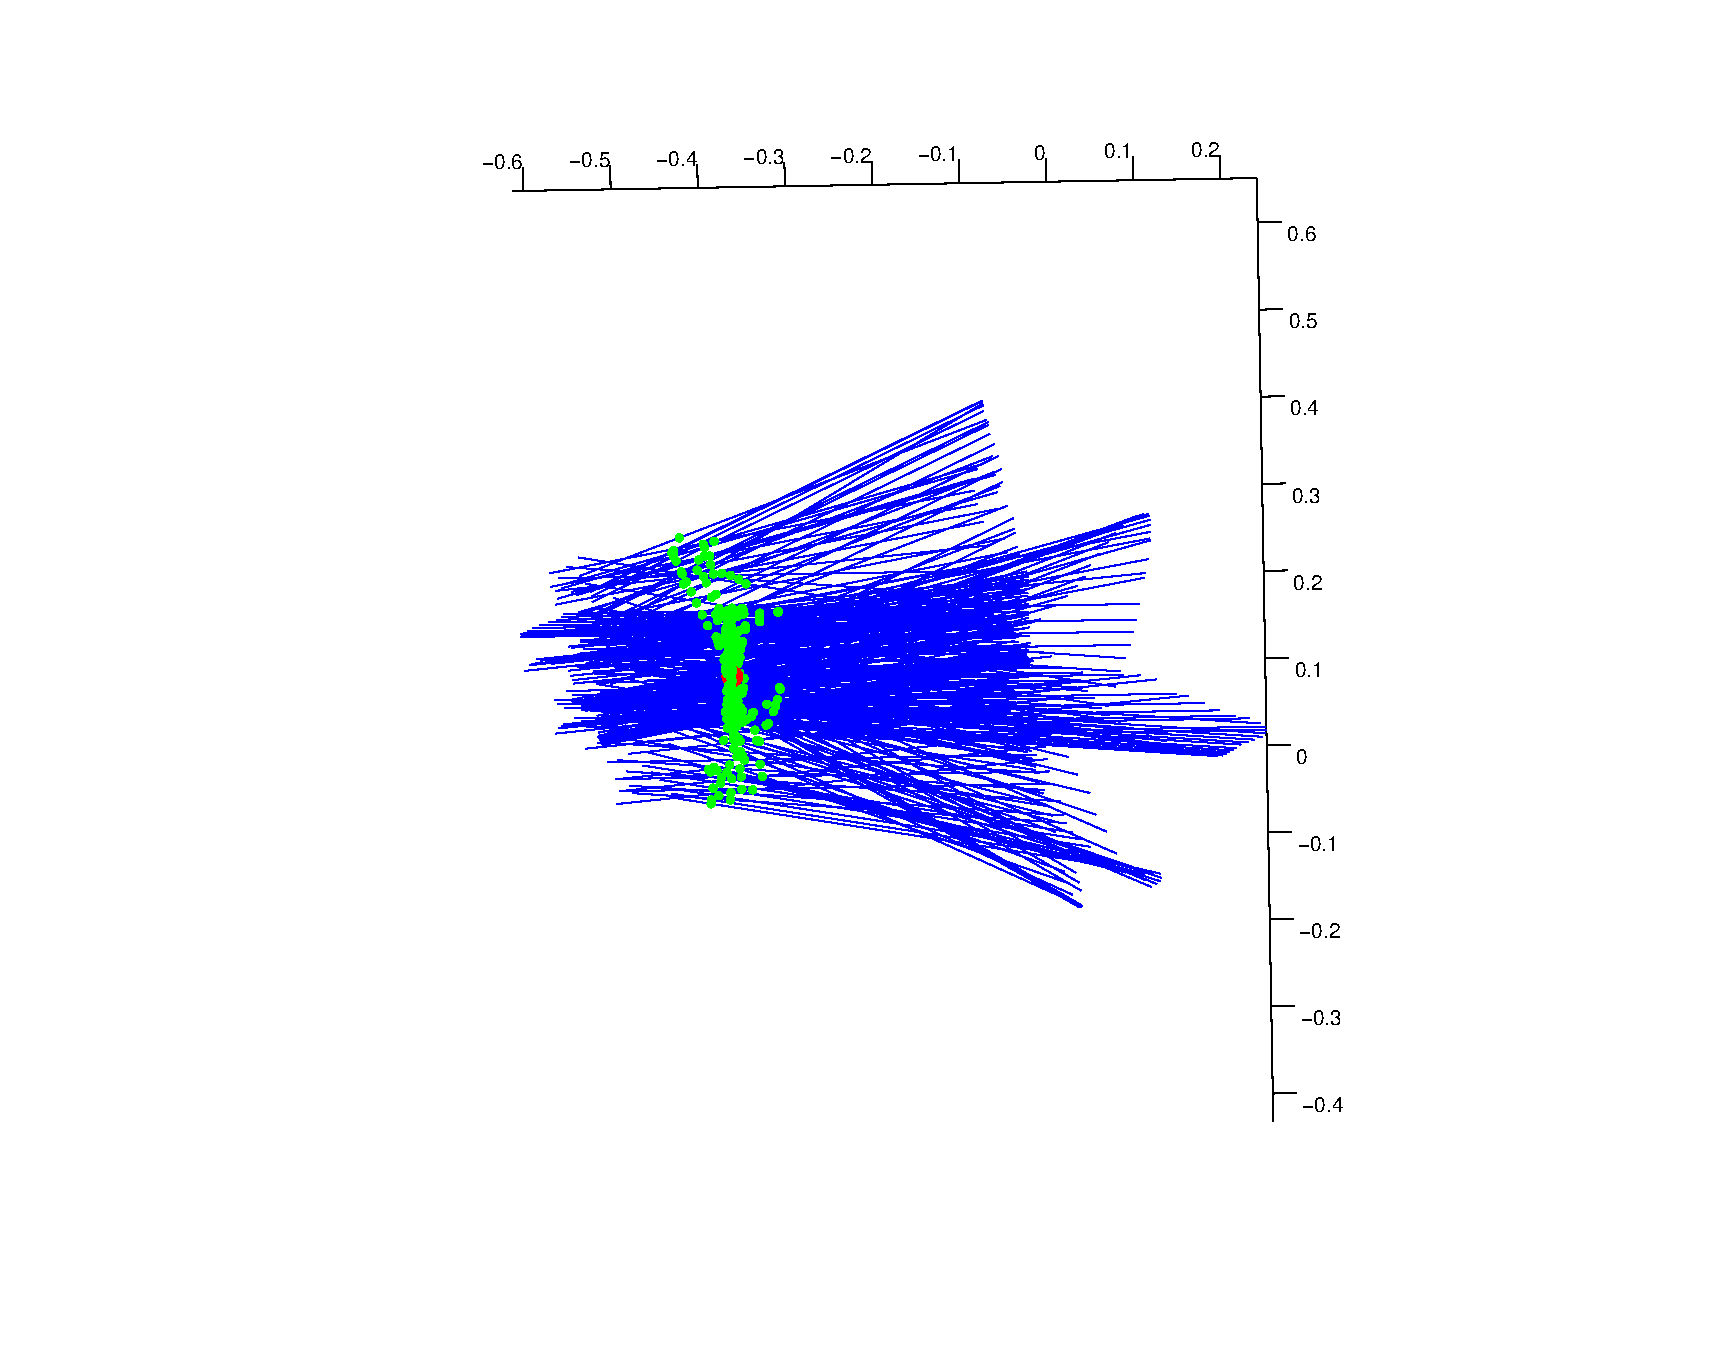
\includegraphics[width=1.1\linewidth]{./img/loc_calib_gauss.eps}
	\end{subfigure}
	\hfill
	\begin{subfigure}[b]{0.49\textwidth}
		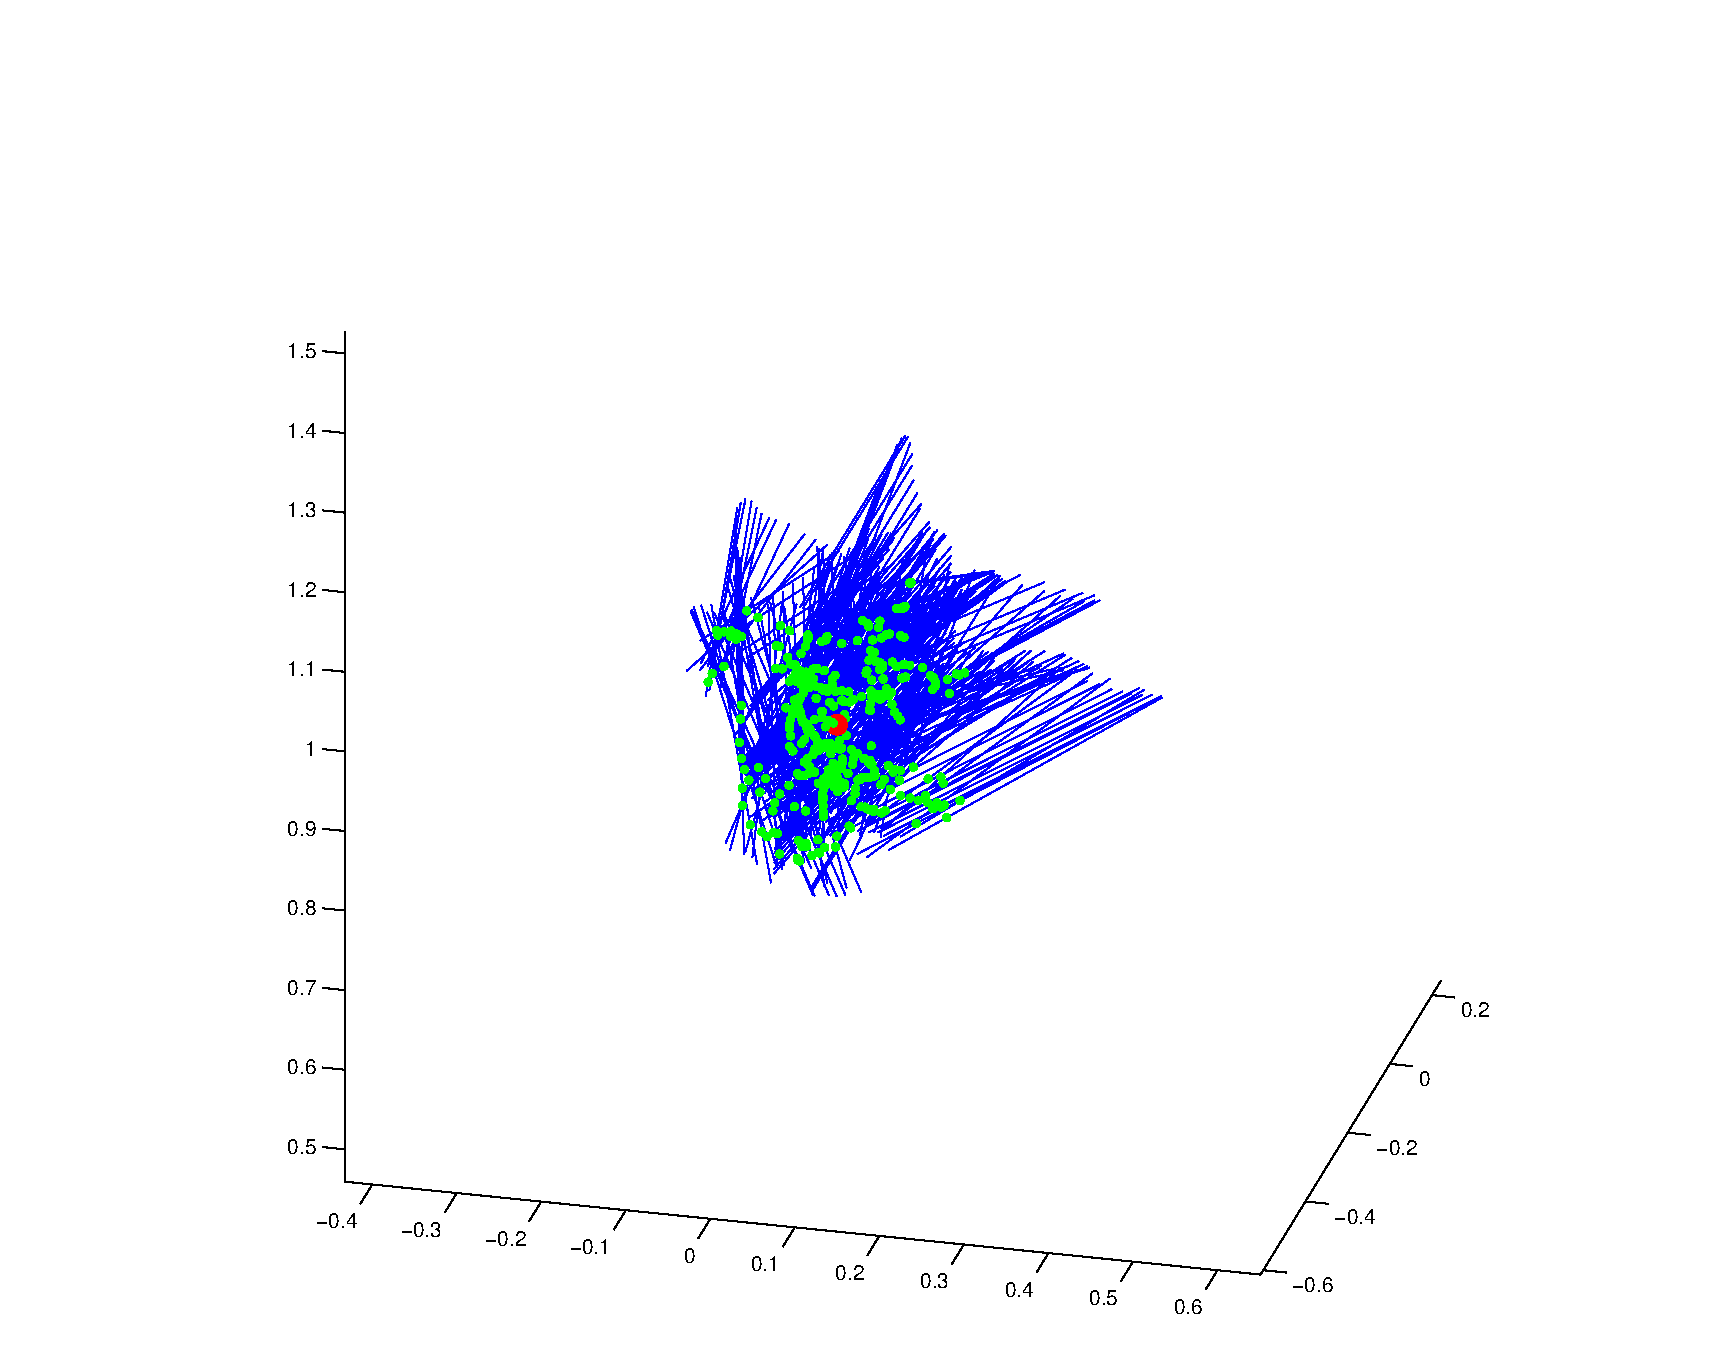
\includegraphics[width=1.1\linewidth]{./img/loc_calib_gauss_cross.eps}
	\end{subfigure}
	\caption{The Gaussian ellipsoid formed by finding the point of minimal sum of squared distances from all gaze lines.  Shown in red is the calculated point, shown in green are the closest point on each gaze line, shown in blue are the gaze lines.  In the left figure, the person doing the object location calibration is standing on the right, looking to the left.  The figure on the right shows the same plot rotated so the spread of the ellipsoid is seen more clearly.}
	\label{fig:locCalibResults}
\end{figure}

After this calibration for the objects of interest, we use a simple heuristic when identifying the object under gaze.  If gaze direction lies within x variance away from an object location mean, then this object is considered to be gazed at (x is a sensitivity parameter chosen manually).  If the gaze lies in two or more objects' vicinities, the object whose distance from gaze normalized by variance is less is chosen as the object under gaze.  If no objects are close to the gaze direction, the person is considered not looking at any object, i.e. idling.

\section{Discussion}
We have shown working implementations of the KinFu algorithm that produces inverse head pose transformed color eye images.  However, due to limitation of time, its capability was not explored.  We did test it with Kinect video footages we have obtained of the child with ASD's head during his hand-washing trials.  However, because the Kinect camera was placed too close to the participant's face (due to limitation of space near the sink), and because the participant rocks back and forth quite rapidly, our algorithm could not track the participant's head motions robustly.  Thus, we weren't able to build a head model from the footages, and thus further investigation was impeded.

For future studies, we need to first ensure the head tracker we developed works with children with ASD.  To do this, we should characterize children with ASD's head movement during hand-washing with the robot, since some children with ASD exhibit rocking motions.  We should note the speed and range of motions.  We may need to reposition the Kinect camera further away from the child to make sure the child's head motions does not go out of camera's range.  Then we need to characterize our head tracker's capability and make sure it can handle children with ASD's head movements.  If the head movements of children with ASD are faster than the tracker can handle, we may consider decreasing the number of vertices in the head model mesh to increase frame rate.

After obtaining a head tracker that works with children with ASD, we can move on to implementing the eye tracker.  Training eye images can be obtained by using the head tracker, doing the frontal pose transformation, and cropping the eye region using the EYEDIAP dataset.  Then the eye tracker can be implemented following the ALR method outlined previously.

For the future studies, one should evaluate the gaze (head plus eye) tracking accuracy for children with ASD.  One way to evaluate it is by letting children with ASD wear a commercially available gaze tracking headset that gives the ground truth of their gaze, and compare it with the gaze direction estimated by our head plus eye tracker.  However, if asking children with ASD to wear the obtrusive headset proves infeasible, then maybe a fun activity can be designed instead that asks children with ASD to look at a moving object (e.g. a ball) whose 3D position can be automatically estimated using Kinect, serving as ground truth.

Lastly, the future studies should integrate the head and eye tracker with object under gaze estimator to realize the VFOA tracker, tracking the object under gaze in real-time.  Robot behaviors responding to child's gaze should then be implemented.  A study evaluating the effectiveness of implemented gaze behavior dependent robot actions on children with ASD's engagement, prompt compliance, and step completion during hand-washing prompting should be conducted.
\chapter{Conclusion}
In this thesis, we aimed to investigate a new modality of interaction for COACH, using a humanoid robot NAO, during the prompting of hand-washing steps to a child with ASD.  A Wizard of Oz (WoZ) study was conducted, and yielded promising results.  In addition, we further improved COACH by implementing a Visual Focus of Attention (VFOA) tracker.  The thesis answers the hypotheses raised in the following way (the hypotheses are shown in bold):

\paragraph{The humanoid robot, NAO, is able to independently assist child with ASD through hand-washing, and child exhibits greater engagement level, higher prompt compliance rate, and better task completion when prompted by NAO than by parent.}
Through the WoZ study, we have seen that NAO was effective in facilitating task completion, though the parent was more effective.  Also, NAO had a low prompt compliance rate compared to the parent during the first phase it was introduced, but through a training phase of joint prompting with the parent, NAO resulted in a higher prompt compliance rate, comparable to that of the parent's.  The measures employed for engagement level (i.e. Number of Times Child Smiles, Number of Times Child Murmurs, Looking at Robot/Parent Rate) were very noisy, and the parent mostly had higher levels than the robot.  We did not observe any correlations between these measures to prompt compliance rate either.  In whole, although we have not achieved totally independent assistance using NAO, we have shown that NAO has very good potential of achieving independent assistance, given longer training and testing sessions.

\paragraph{Gestural, gaze, and verbal are the essential modes of interactions present in the hand-washing prompting scenario between child with ASD and the prompting agent NAO.}
The WoZ study revealed that verbal instructions and pointing gestures are useful for our participant, who knows the execution of each hand-washing step, but needs reminders of which step to execute.  In cases the child did need demonstrations for a step, NAO's limited dexterity made the motion demonstration somewhat confusing to the child compared to that of the parent's.  In terms of gaze behaviors during interactions, our participant generally avoided looking at the prompting agent when he knew what to do, and tends to look at the parent more than NAO when seeking help.  Lastly, when the child is not complying, the parent had the ability to increase the invasiveness of the prompt by physically influencing the child through nudging, guiding the arm, and fully doing the step hand-on-hand.  This increase of physical invasiveness was effective in promoting compliance, and NAO lacked such interaction modality.

\paragraph{Using 3DMM and ALR for estimating head pose and eye pose, and using the Kinect camera, a classification rate of more than 80\% is achieved for estimating child's VFOA on NAO, monitor screen, soap, towel, tap region, hands, and idling.}
We have implemented the head pose tracker using the Kinect camera, employing our modified version of the KinFu algorithm.  However, due to rapid head movements of the participant during hand-washing sessions, our head pose tracker was not successful in tracking his head.  Future improvements were suggested.  We have also implemented front-pose transformation of the head image for eye region cropping.  But due to limitation of time, we did not implement the eye pose tracker using EYEDIAP dataset employing the ALR method.  Lastly, we implemented the object under gaze estimator.  In whole, we showed the feasibility of implementing the VFOA's three components (i.e. head pose tracker, eye pose tracker, object under gaze estimator), and described the steps for completing its implementation and evaluating its performance.
\\
\\
In conclusion, the thesis results suggest promising prospects of utilizing the humanoid, NAO, as a novel prompting modality to enhance COACH, and to fill the gap of in-vivo ATCs for teaching daily skills that can automatically deliver prompts and reinforcement schedules.  Future investigations in regards to improving the child's engagement further through more creative design of the robot's appearance and behavior dynamics were suggested.  One such improvement could come from implementing robot behaviors contingent to the VFOA of the child.

%special thanks to: Jiayang Jiang, Leon Li, Jimmy, Boyu and Betty, Andrew and others at CEACT
%thank prof, thank Bing, Tuck, and other lab members
%thank committee members


%% This adds a line for the Bibliography in the Table of Contents.
\addcontentsline{toc}{chapter}{Bibliography}
%% *** Set the bibliography style. ***
%% (change according to your preference/requirements)
\bibliographystyle{plain}
%% *** Set the bibliography file. ***
%% ("thesis.bib" by default; change as needed)
\begin{thebibliography}{100}

\bibitem{abledata2010alpha}
{AbleData} alpha interactive language series—gator super sentences.
\newblock \url{http://www.abledata.com}.
\newblock Accessed: July 18, 2010.

\bibitem{autism2014facts}
{Autism Speaks Canada} facts and stats.
\newblock
  \url{http://www.autismservicesinc.com/pdf/Autism%20Speaks%20Canada%20Updated%20Facts%20and%20Stats.pdf}.
\newblock Accessed: June 20, 2015.

\bibitem{mackiev2010welcome}
{MacKiev.com} welcome to roger wagner’s hyperstudio.
\newblock \url{http://www.mackiev.com/hyperstudio}.
\newblock Accessed: September 27, 2010.

\bibitem{synapse2010the}
{Synapse Adaptive} the therapy tool that has people talking.
\newblock \url{http://www.synapseadaptive.com/edmark/prod/sv3}.
\newblock Accessed: July 20, 2010.

\bibitem{1997microsoft}
Microsoft powerpoint [computer software].
\newblock {\em Redmond, WA: Microsoft Corporation}, 1997–2003.

\bibitem{2005team}
Team up with timo: Animated learning tutor. [computer software].
\newblock {\em San Francisco, CA: Animated Speech Corporation}, 2005.

\bibitem{amberg2008expression}
Brian Amberg, Reinhard Knothe, and Thomas Vetter.
\newblock Expression invariant 3d face recognition with a morphable model.
\newblock In {\em Automatic Face \& Gesture Recognition, 2008. FG'08. 8th IEEE
  International Conference on}, pages 1--6. IEEE, 2008.

\bibitem{ayres2009acquisition}
Kevin~M Ayres, Amy Maguire, and Desiree McClimon.
\newblock Acquisition and generalization of chained tasks taught with computer
  based video instruction to children with autism.
\newblock {\em Education and Training in Developmental Disabilities},
  44(4):493, 2009.

\bibitem{baluja1994non}
Shumeet Baluja and Dean Pomerleau.
\newblock Non-intrusive gaze tracking using artificial neural networks.
\newblock Technical report, DTIC Document, 1994.

\bibitem{bandura1969principles}
Albert Bandura.
\newblock Principles of behavior modification.
\newblock 1969.

\bibitem{belkin2003laplacian}
Mikhail Belkin and Partha Niyogi.
\newblock Laplacian eigenmaps for dimensionality reduction and data
  representation.
\newblock {\em Neural computation}, 15(6):1373--1396, 2003.

\bibitem{bellini2007meta}
Scott Bellini and Jennifer Akullian.
\newblock A meta-analysis of video modeling and video self-modeling
  interventions for children and adolescents with autism spectrum disorders.
\newblock {\em Exceptional children}, 73(3):264--287, 2007.

\bibitem{bereznak2012video}
Sally Bereznak, Kevin~M Ayres, Linda~C Mechling, and Jennifer~L Alexander.
\newblock Video self-prompting and mobile technology to increase daily living
  and vocational independence for students with autism spectrum disorders.
\newblock {\em Journal of Developmental and Physical Disabilities},
  24(3):269--285, 2012.

\bibitem{bernard1999enhancing}
Vera Bernard-Opitz, N~Sriram, and Sharul Sapuan.
\newblock Enhancing vocal imitations in children with autism using the ibm
  speech viewer.
\newblock {\em Autism}, 3(2):131--147, 1999.

\bibitem{bertalmio2000image}
Marcelo Bertalmio, Guillermo Sapiro, Vincent Caselles, and Coloma Ballester.
\newblock Image inpainting.
\newblock In {\em Proceedings of the 27th annual conference on Computer
  graphics and interactive techniques}, pages 417--424. ACM
  Press/Addison-Wesley Publishing Co., 2000.

\bibitem{bhargava2013demonstration}
Shweta Bhargava, Srinivasan Janarthanam, Helen Hastie, Amol Deshmukh, Ruth
  Aylett, Lee Corrigan, and Ginevra Castellano.
\newblock Demonstration of the emote wizard of oz interface for empathic
  robotic tutors.
\newblock In {\em Proceedings of SIGdial}, 2013.

\bibitem{bimbrahw2012investigating}
Justin Bimbrahw, Jennifer Boger, and Alex Mihailidis.
\newblock Investigating the efficacy of a computerized prompting device to
  assist children with autism spectrum disorder with activities of daily
  living.
\newblock {\em Assistive Technology}, 24(4):286--298, 2012.

\bibitem{bogin2010steps}
J~Bogin, L~Sullivan, S~Rogers, A~Stabel, and D~Hatton.
\newblock Steps for implementation: Discrete trial training, 2010.

\bibitem{bondy1994picture}
Andrew~S Bondy and Lori~A Frost.
\newblock The picture exchange communication system.
\newblock {\em Focus on Autism and Other Developmental Disabilities},
  9(3):1--19, 1994.

\bibitem{bosseler2003development}
Alexis Bosseler and Dominic~W Massaro.
\newblock Development and evaluation of a computer-animated tutor for
  vocabulary and language learning in children with autism.
\newblock {\em Journal of autism and developmental disorders}, 33(6):653--672,
  2003.

\bibitem{buggey2005video}
Tom Buggey.
\newblock Video self-modeling applications with students with autism spectrum
  disorder in a small private school setting.
\newblock {\em Focus on autism and other developmental disabilities},
  20(1):52--63, 2005.

\bibitem{buggey1999training}
Tom Buggey, Kristina Toombs, Pia Gardener, and Michele Cervetti.
\newblock Training responding behaviors in students with autism using
  videotaped self-modeling.
\newblock {\em Journal of Positive Behavior Interventions}, 1(4):205--214,
  1999.

\bibitem{burgess2007quality}
Audrey~F Burgess and Steven~E Gutstein.
\newblock Quality of life for people with autism: Raising the standard for
  evaluating successful outcomes.
\newblock {\em Child and Adolescent Mental Health}, 12(2):80--86, 2007.

\bibitem{case2008evidence}
Jane Case-Smith and Marian Arbesman.
\newblock Evidence-based review of interventions for autism used in or of
  relevance to occupational therapy.
\newblock {\em American Journal of Occupational Therapy}, 62(4):416--429, 2008.

\bibitem{cohen2006early}
Howard Cohen, Mila Amerine-Dickens, and Tristram Smith.
\newblock Early intensive behavioral treatment: Replication of the ucla model
  in a community setting.
\newblock {\em Journal of Developmental \& Behavioral Pediatrics},
  27(2):S145--S155, 2006.

\bibitem{coleman2005using}
Mari~Beth Coleman-Martin, Kathryn~Wolff Heller, David~F Cihak, and Kathryn~L
  Irvine.
\newblock Using computer-assisted instruction and the nonverbal reading
  approach to teach word identification.
\newblock {\em Focus on Autism and Other Developmental Disabilities},
  20(2):80--90, 2005.

\bibitem{colombo1999real}
Carlo Colombo and Alberto Del~Bimbo.
\newblock Real-time head tracking from the deformation of eye contours using a
  piecewise affine camera.
\newblock {\em Pattern Recognition Letters}, 20(7):721--730, 1999.

\bibitem{constantino2002social}
John~N Constantino and Christian~P Gruber.
\newblock The social responsiveness scale.
\newblock {\em Los Angeles: Western Psychological Services}, 2002.

\bibitem{dautenhahn2004towards}
Kerstin Dautenhahn and Iain Werry.
\newblock Towards interactive robots in autism therapy: Background, motivation
  and challenges.
\newblock {\em Pragmatics \& Cognition}, 12(1):1--35, 2004.

\bibitem{diehl2012clinical}
Joshua~J Diehl, Lauren~M Schmitt, Michael Villano, and Charles~R Crowell.
\newblock The clinical use of robots for individuals with autism spectrum
  disorders: A critical review.
\newblock {\em Research in autism spectrum disorders}, 6(1):249--262, 2012.

\bibitem{duquette2008exploring}
Audrey Duquette, Fran{\c{c}}ois Michaud, and Henri Mercier.
\newblock Exploring the use of a mobile robot as an imitation agent with
  children with low-functioning autism.
\newblock {\em Autonomous Robots}, 24(2):147--157, 2008.

\bibitem{feil2005defining}
David Feil-Seifer and Maja~J Mataric.
\newblock Defining socially assistive robotics.
\newblock In {\em Rehabilitation Robotics, 2005. ICORR 2005. 9th International
  Conference on}, pages 465--468. IEEE, 2005.

\bibitem{feil2009toward}
David Feil-Seifer and Maja~J Matari{\'c}.
\newblock Toward socially assistive robotics for augmenting interventions for
  children with autism spectrum disorders.
\newblock In {\em Experimental robotics}, pages 201--210. Springer, 2009.

\bibitem{fong2003survey}
Terrence Fong, Illah Nourbakhsh, and Kerstin Dautenhahn.
\newblock A survey of socially interactive robots.
\newblock {\em Robotics and autonomous systems}, 42(3):143--166, 2003.

\bibitem{foxx1982decreasing}
Richard~M Foxx.
\newblock {\em Decreasing behaviors of severely retarded and autistic persons}.
\newblock Research Press, 1982.

\bibitem{foxx2008applied}
Richard~M Foxx.
\newblock Applied behavior analysis treatment of autism: The state of the art.
\newblock {\em Child and adolescent psychiatric clinics of North America},
  17(4):821--834, 2008.

\bibitem{francis2005autism}
K~Francis.
\newblock Autism interventions: a critical update.
\newblock {\em Developmental Medicine \& Child Neurology}, 47(7):493--499,
  2005.

\bibitem{frank2004assistive}
Edmund Frank~Lopresti, Alex Mihailidis, and Ned Kirsch.
\newblock Assistive technology for cognitive rehabilitation: State of the art.
\newblock {\em Neuropsychological rehabilitation}, 14(1-2):5--39, 2004.

\bibitem{frith2005autism}
Uta Frith and Francesca Happ{\'e}.
\newblock Autism spectrum disorder.
\newblock {\em Current biology}, 15(19):R786--R790, 2005.

\bibitem{funes2012gaze}
Kenneth~Alberto Funes~Mora and J~Odobez.
\newblock Gaze estimation from multimodal kinect data.
\newblock In {\em Computer Vision and Pattern Recognition Workshops (CVPRW),
  2012 IEEE Computer Society Conference on}, pages 25--30. IEEE, 2012.

\bibitem{funes2013person}
Kenneth~Alberto Funes~Mora and Jean-Marc Odobez.
\newblock Person independent 3d gaze estimation from remote rgb-d cameras.
\newblock In {\em International Conference on Image Processing}, number
  EPFL-CONF-192423. IEEE, 2013.

\bibitem{ganz2012meta}
Jennifer~B Ganz, John~L Davis, Emily~M Lund, Fara~D Goodwyn, and Richard~L
  Simpson.
\newblock Meta-analysis of pecs with individuals with asd: Investigation of
  targeted versus non-targeted outcomes, participant characteristics, and
  implementation phase.
\newblock {\em Research in developmental disabilities}, 33(2):406--418, 2012.

\bibitem{ganz2012metab}
Jennifer~B Ganz, Theresa~L Earles-Vollrath, Amy~K Heath, Richard~I Parker,
  Mandy~J Rispoli, and Jaime~B Duran.
\newblock A meta-analysis of single case research studies on aided augmentative
  and alternative communication systems with individuals with autism spectrum
  disorders.
\newblock {\em Journal of autism and developmental disorders}, 42(1):60--74,
  2012.

\bibitem{ganz2013moderation}
Jennifer~B Ganz, Mandy~J Rispoli, Rose~Ann Mason, and Ee~Rea Hong.
\newblock Moderation of effects of aac based on setting and types of aided aac
  on outcome variables: An aggregate study of single-case research with
  individuals with asd.
\newblock {\em Developmental neurorehabilitation}, 17(3):184--192, 2013.

\bibitem{goldsmith2004use}
Tina~R Goldsmith and Linda~A LeBlanc.
\newblock Use of technology in interventions for children with autism.
\newblock {\em Journal of Early and Intensive Behavior Intervention}, 1(2):166,
  2004.

\bibitem{goodrich2007human}
Michael~A Goodrich and Alan~C Schultz.
\newblock Human-robot interaction: a survey.
\newblock {\em Foundations and trends in human-computer interaction},
  1(3):203--275, 2007.

\bibitem{graetz2006show}
Janet~E Graetz, Margo~A Mastropieri, and Thomas~E Scruggs.
\newblock Show time using video self-modeling to decrease inappropriate
  behavior.
\newblock {\em Teaching exceptional children}, 38(5):43--48, 2006.

\bibitem{hansen2010eye}
Dan~Witzner Hansen and Qiang Ji.
\newblock In the eye of the beholder: A survey of models for eyes and gaze.
\newblock {\em Pattern Analysis and Machine Intelligence, IEEE Transactions
  on}, 32(3):478--500, 2010.

\bibitem{heimann1995increasing}
Mikael Heimann, Keith~E Nelson, Tomas Tjus, and Christopher Gillberg.
\newblock Increasing reading and communication skills in children with autism
  through an interactive multimedia computer program.
\newblock {\em Journal of autism and developmental disorders}, 25(5):459--480,
  1995.

\bibitem{herrera2012joint}
C~Herrera, Juho Kannala, Janne Heikkil{\"a}, et~al.
\newblock Joint depth and color camera calibration with distortion correction.
\newblock {\em Pattern Analysis and Machine Intelligence, IEEE Transactions
  on}, 34(10):2058--2064, 2012.

\bibitem{hetzroni2005logos}
Orit~E Hetzroni and Uri Shalem.
\newblock From logos to orthographic symbols: A multilevel fading computer
  program for teaching nonverbal children with autism.
\newblock {\em Focus on Autism and Other Developmental Disabilities},
  20(4):201--212, 2005.

\bibitem{hetzroni2004effects}
Orit~E Hetzroni and Juman Tannous.
\newblock Effects of a computer-based intervention program on the communicative
  functions of children with autism.
\newblock {\em Journal of autism and developmental disorders}, 34(2):95--113,
  2004.

\bibitem{hine2006using}
Jeffrey~F Hine and Mark Wolery.
\newblock Using point-of-view video modeling to teach play to preschoolers with
  autism.
\newblock {\em Topics in Early Childhood Special Education}, 26(2):83--93,
  2006.

\bibitem{hitchcock2003video}
Caryl~H Hitchcock, Peter~W Dowrick, and Mary~Anne Prater.
\newblock Video self-modeling intervention in school-based settings a review.
\newblock {\em Remedial and Special Education}, 24(1):36--45, 2003.

\bibitem{howlin2003outcome}
Patricia Howlin.
\newblock Outcome in high-functioning adults with autism with and without early
  language delays: implications for the differentiation between autism and
  asperger syndrome.
\newblock {\em Journal of autism and developmental disorders}, 33(1):3--13,
  2003.

\bibitem{howlin2009systematic}
Patricia Howlin, Iliana Magiati, and Tony Charman.
\newblock Systematic review of early intensive behavioral interventions for
  children with autism.
\newblock {\em Journal Information}, 114(1), 2009.

\bibitem{hutcherson2004computer}
Karen Hutcherson, John Langone, Kevin Ayres, and Tom Clees.
\newblock Computer assisted instruction to teach item selection in grocery
  stores: An assessment of acquisition and generalization.
\newblock {\em Journal of Special Education Technology}, 19(4):33--42, 2004.

\bibitem{kagohara2013using}
Debora~M Kagohara, Larah van~der Meer, Sathiyaprakash Ramdoss, Mark~F
  O’Reilly, Giulio~E Lancioni, Tonya~N Davis, Mandy Rispoli, Russell Lang,
  Peter~B Marschik, Dean Sutherland, et~al.
\newblock Using ipods{\textregistered} and ipads{\textregistered} in teaching
  programs for individuals with developmental disabilities: A systematic
  review.
\newblock {\em Research in developmental disabilities}, 34(1):147--156, 2013.

\bibitem{kim2001second}
Sunyonga Kim and Masakazu Kojima.
\newblock Second order cone programming relaxation of nonconvex quadratic
  optimization problems.
\newblock {\em Optimization Methods and Software}, 15(3-4):201--224, 2001.

\bibitem{kogan2009prevalence}
Michael~D Kogan, Stephen~J Blumberg, Laura~A Schieve, Coleen~A Boyle, James~M
  Perrin, Reem~M Ghandour, Gopal~K Singh, Bonnie~B Strickland, Edwin Trevathan,
  and Peter~C van Dyck.
\newblock Prevalence of parent-reported diagnosis of autism spectrum disorder
  among children in the us, 2007.
\newblock {\em Pediatrics}, 124(5):1395--1403, 2009.

\bibitem{kruger2002gabor}
Volker Kr{\"u}ger and Gerald Sommer.
\newblock Gabor wavelet networks for efficient head pose estimation.
\newblock {\em Image and vision computing}, 20(9):665--672, 2002.

\bibitem{lang2014assistive}
Russell Lang, Sathiyaprakash Ramdoss, Tracy Raulston, Amarie Carnet, Jeff
  Sigafoos, Robert Didden, Dennis Moore, and Mark~F O’Reilly.
\newblock Assistive technology for people with autism spectrum disorders.
\newblock In {\em Assistive Technologies for People with Diverse Abilities},
  pages 157--190. Springer, 2014.

\bibitem{li2000support}
Yongmin Li, Shaogang Gong, and Heather Liddell.
\newblock Support vector regression and classification based multi-view face
  detection and recognition.
\newblock In {\em Automatic Face and Gesture Recognition, 2000. Proceedings.
  Fourth IEEE International Conference on}, pages 300--305. IEEE, 2000.

\bibitem{liss2001predictors}
Miriam Liss, Brian Harel, Deborah Fein, Doris Allen, Michelle Dunn, Carl
  Feinstein, Robin Morris, Lynn Waterhouse, and Isabel Rapin.
\newblock Predictors and correlates of adaptive functioning in children with
  developmental disorders.
\newblock {\em Journal of autism and developmental disorders}, 31(2):219--230,
  2001.

\bibitem{lovaas1987behavioral}
O~Ivar Lovaas.
\newblock Behavioral treatment and normal educational and intellectual
  functioning in young autistic children.
\newblock {\em Journal of consulting and clinical psychology}, 55(1):3, 1987.

\bibitem{lovaas1979stimulus}
O~Ivar Lovaas, Robert~L Koegel, and Laura Schreibman.
\newblock Stimulus overselectivity in autism: A review of research.
\newblock {\em Psychological bulletin}, 86(6):1236, 1979.

\bibitem{low2004linear}
Kok-Lim Low.
\newblock Linear least-squares optimization for point-to-plane icp surface
  registration.
\newblock {\em Chapel Hill, University of North Carolina}, 2004.

\bibitem{lu2011inferring}
Feng Lu, Yusuke Sugano, Takahiro Okabe, and Yoichi Sato.
\newblock Inferring human gaze from appearance via adaptive linear regression.
\newblock In {\em Computer Vision (ICCV), 2011 IEEE International Conference
  on}, pages 153--160. IEEE, 2011.

\bibitem{massaro2006read}
Dominic~W Massaro and Alexis Bosseler.
\newblock Read my lips the importance of the face in a computer-animated tutor
  for vocabulary learning by children with autism.
\newblock {\em Autism}, 10(5):495--510, 2006.

\bibitem{mataric2005role}
Maja~J Mataric.
\newblock The role of embodiment in assistive interactive robotics for the
  elderly.
\newblock In {\em AAAI fall symposium on caring machines: AI for the elderly,
  Arlington, VA}, 2005.

\bibitem{mechling2010computer}
Linda Mechling and Eileen O'Brien.
\newblock Computer-based video instruction to teach students with intellectual
  disabilities to use public bus transportation.
\newblock {\em Education and Training in Autism and Developmental
  Disabilities}, pages 230--241, 2010.

\bibitem{mihailidis2008coach}
Alex Mihailidis, Jennifer~N Boger, Tammy Craig, and Jesse Hoey.
\newblock The coach prompting system to assist older adults with dementia
  through handwashing: An efficacy study.
\newblock {\em BMC geriatrics}, 8(1):28, 2008.

\bibitem{mirenda2001autism}
Pat Mirenda.
\newblock Autism, augmentative communication, and assistive technology what do
  we really know?
\newblock {\em Focus on Autism and Other Developmental Disabilities},
  16(3):141--151, 2001.

\bibitem{moore2000brief}
Monique Moore and Sandra Calvert.
\newblock Brief report: Vocabulary acquisition for children with autism:
  Teacher or computer instruction.
\newblock {\em Journal of autism and developmental disorders}, 30(4):359--362,
  2000.

\bibitem{mora2014eyediap}
Kenneth Alberto~Funes Mora, Florent Monay, and Jean-Marc Odobez.
\newblock Eyediap: a database for the development and evaluation of gaze
  estimation algorithms from rgb and rgb-d cameras.
\newblock In {\em Proceedings of the Symposium on Eye Tracking Research and
  Applications}, pages 255--258. ACM, 2014.

\bibitem{murphy2009head}
Erik Murphy-Chutorian and Mohan~M Trivedi.
\newblock Head pose estimation in computer vision: A survey.
\newblock {\em Pattern Analysis and Machine Intelligence, IEEE Transactions
  on}, 31(4):607--626, 2009.

\bibitem{newcombe2011kinectfusion}
Richard~A Newcombe, Shahram Izadi, Otmar Hilliges, David Molyneaux, David Kim,
  Andrew~J Davison, Pushmeet Kohi, Jamie Shotton, Steve Hodges, and Andrew
  Fitzgibbon.
\newblock Kinectfusion: Real-time dense surface mapping and tracking.
\newblock In {\em Mixed and augmented reality (ISMAR), 2011 10th IEEE
  international symposium on}, pages 127--136. IEEE, 2011.

\bibitem{parsons1993effect}
Carl~L Parsons and Diane La~Sorte.
\newblock The effect of computers with synthesized speech and no speech on the
  spontaneous communication of children with autism.
\newblock {\em Australian Journal of Human Communication Disorders},
  21(1):12--31, 1993.

\bibitem{paysan20093d}
Pascal Paysan, Reinhard Knothe, Brian Amberg, Sami Romdhani, and Thomas Vetter.
\newblock A 3d face model for pose and illumination invariant face recognition.
\newblock In {\em Advanced Video and Signal Based Surveillance, 2009. AVSS'09.
  Sixth IEEE International Conference On}, pages 296--301. IEEE, 2009.

\bibitem{pierno2008robotic}
Andrea~C Pierno, Morena Mari, Dean Lusher, and Umberto Castiello.
\newblock Robotic movement elicits visuomotor priming in children with autism.
\newblock {\em Neuropsychologia}, 46(2):448--454, 2008.

\bibitem{pirovano2011kinfu}
M.~Pirovano.
\newblock Kinfu – an open-source implementation of kinect fusion + case
  study: Implementing a 3d scanner with pcl.
\newblock {\em 3D Structure from Visual Motion}, 2011/2012.

\bibitem{preston2009review}
Deborah Preston and Mark Carter.
\newblock A review of the efficacy of the picture exchange communication system
  intervention.
\newblock {\em Journal of autism and developmental disorders},
  39(10):1471--1486, 2009.

\bibitem{ramdoss2011use}
Sathiyaprakash Ramdoss, Russell Lang, Austin Mulloy, Jessica Franco, Mark
  O’Reilly, Robert Didden, and Giulio Lancioni.
\newblock Use of computer-based interventions to teach communication skills to
  children with autism spectrum disorders: A systematic review.
\newblock {\em Journal of Behavioral Education}, 20(1):55--76, 2011.

\bibitem{ramdoss2012computer}
Sathiyaprakash Ramdoss, Wendy Machalicek, Mandy Rispoli, Austin Mulloy, Russell
  Lang, and Mark O'Reilly.
\newblock Computer-based interventions to improve social and emotional skills
  in individuals with autism spectrum disorders: A systematic review.
\newblock {\em Developmental Neurorehabilitation}, 15(2):119--135, 2012.

\bibitem{ramdoss2011useb}
Sathiyaprakash Ramdoss, Austin Mulloy, Russell Lang, Mark O’Reilly, Jeff
  Sigafoos, Giulio Lancioni, Robert Didden, and Farah El~Zein.
\newblock Use of computer-based interventions to improve literacy skills in
  students with autism spectrum disorders: A systematic review.
\newblock {\em Research in Autism Spectrum Disorders}, 5(4):1306--1318, 2011.

\bibitem{rao2008social}
Patricia~A Rao, Deborah~C Beidel, and Michael~J Murray.
\newblock Social skills interventions for children with asperger’s syndrome
  or high-functioning autism: A review and recommendations.
\newblock {\em Journal of autism and developmental disorders}, 38(2):353--361,
  2008.

\bibitem{ravindra2009therapeutic}
P~Ravindra, S~De~Silva, Katsunori Tadano, Azusa Saito, Stephen~G Lambacher, and
  Mastake Higashi.
\newblock Therapeutic-assisted robot for children with autism.
\newblock In {\em Intelligent Robots and Systems, 2009. IROS 2009. IEEE/RSJ
  International Conference on}, pages 3561--3567. IEEE, 2009.

\bibitem{raytchev2004head}
Bisser Raytchev, Ikushi Yoda, and Katsuhiko Sakaue.
\newblock Head pose estimation by nonlinear manifold learning.
\newblock In {\em Pattern Recognition, 2004. ICPR 2004. Proceedings of the 17th
  International Conference on}, volume~4, pages 462--466. IEEE, 2004.

\bibitem{reinders1996locating}
Marcel~JT Reinders, RWC Koch, and Jan~J Gerbrands.
\newblock Locating facial features in image sequences using neural networks.
\newblock In {\em Automatic Face and Gesture Recognition, 1996., Proceedings of
  the Second International Conference on}, pages 230--235. IEEE, 1996.

\bibitem{robins2006does}
Ben Robins, Kerstin Dautenhahn, and Janek Dubowski.
\newblock Does appearance matter in the interaction of children with autism
  with a humanoid robot?
\newblock {\em Interaction Studies}, 7(3):509--542, 2006.

\bibitem{robins2005robotic}
Ben Robins, Kerstin Dautenhahn, R~Te~Boekhorst, and Aude Billard.
\newblock Robotic assistants in therapy and education of children with autism:
  can a small humanoid robot help encourage social interaction skills?
\newblock {\em Universal Access in the Information Society}, 4(2):105--120,
  2005.

\bibitem{rosenberg2010evaluating}
Nancy~E Rosenberg, Ilene~S Schwartz, and Carol~A Davis.
\newblock Evaluating the utility of commercial videotapes for teaching hand
  washing to children with autism.
\newblock {\em Education and Treatment of Children}, 33(3):443--455, 2010.

\bibitem{roweis2000nonlinear}
Sam~T Roweis and Lawrence~K Saul.
\newblock Nonlinear dimensionality reduction by locally linear embedding.
\newblock {\em Science}, 290(5500):2323--2326, 2000.

\bibitem{rusu20113d}
Radu~Bogdan Rusu and Steve Cousins.
\newblock 3d is here: Point cloud library (pcl).
\newblock In {\em Robotics and Automation (ICRA), 2011 IEEE International
  Conference on}, pages 1--4. IEEE, 2011.

\bibitem{sallows2005intensive}
Glen~O Sallows and Tamlynn~D Graupner.
\newblock Intensive behavioral treatment for children with autism: Four-year
  outcome and predictors.
\newblock {\em Journal Information}, 110(6), 2005.

\bibitem{scheuermann2002teaching}
B.~Scheuermann and J.~Webber.
\newblock Teaching does make a difference.
\newblock {\em Belmont: Wadsworth/Thomson Learning}, 2002.

\bibitem{schlosser2008effects}
Ralf~W Schlosser and Oliver Wendt.
\newblock Effects of augmentative and alternative communication intervention on
  speech production in children with autism: A systematic review.
\newblock {\em American Journal of Speech-Language Pathology}, 17(3):212--230,
  2008.

\bibitem{shabani2002increasing}
Daniel~B Shabani, Roger~C Katz, David~A Wilder, Kenneth Beauchamp, Crystal~R
  Taylor, and Kirsten~J Fischer.
\newblock Increasing social initiations in children with autism: Effects of a
  tactile prompt.
\newblock {\em Journal of Applied Behavior Analysis}, 35(1):79--83, 2002.

\bibitem{shane2012applying}
Howard~C Shane, Emily~H Laubscher, Ralf~W Schlosser, Suzanne Flynn, James~F
  Sorce, and Jennifer Abramson.
\newblock Applying technology to visually support language and communication in
  individuals with autism spectrum disorders.
\newblock {\em Journal of autism and developmental disorders},
  42(6):1228--1235, 2012.

\bibitem{shipley2002teaching}
Robin Shipley-Benamou, John~R Lutzker, and Mitchell Taubman.
\newblock Teaching daily living skills to children with autism through
  instructional video modeling.
\newblock {\em Journal of Positive Behavior Interventions}, 4(3):166--177,
  2002.

\bibitem{shukla2009evaluating}
Smita Shukla-Mehta, Trube Miller, and Kevin~J Callahan.
\newblock Evaluating the effectiveness of video instruction on social and
  communication skills training for children with autism spectrum disorders: A
  review of the literature.
\newblock {\em Focus on Autism and Other Developmental Disabilities}, 2009.

\bibitem{sigafoos2001conditional}
Jeff Sigafoos and Erik Drasgow.
\newblock Conditional use of aided and unaided aac a review and clinical case
  demonstration.
\newblock {\em Focus on Autism and Other Developmental Disabilities},
  16(3):152--161, 2001.

\bibitem{sigafoos2007assessing}
Jeff Sigafoos, Jennifer~B Ganz, Mark O’Reilly, Giulio~E Lancioni, and Ralf~W
  Schlosser.
\newblock Assessing correspondence following acquisition of an exchange-based
  communication system.
\newblock {\em Research in Developmental Disabilities}, 28(1):71--83, 2007.

\bibitem{sigafoos2007evaluation}
Jeff Sigafoos, Mark O’Reilly, Helen Cannella, Chaturi Edrisinha, Berenice
  de~la Cruz, Megha Upadhyaya, Giulio~E Lancioni, Anna Hundley, Alonzo Andrews,
  Carolyn Garver, et~al.
\newblock Evaluation of a video prompting and fading procedure for teaching
  dish washing skills to adults with developmental disabilities.
\newblock {\em Journal of Behavioral Education}, 16(2):93--109, 2007.

\bibitem{sigafoos2005computer}
Jeff Sigafoos, Mark O’Reilly, Helen Cannella, Megha Upadhyaya, Chaturi
  Edrisinha, Giulio~E Lancioni, Anna Hundley, Alonzo Andrews, Carolyn Garver,
  and David Young.
\newblock Computer-presented video prompting for teaching microwave oven use to
  three adults with developmental disabilities.
\newblock {\em Journal of Behavioral Education}, 14(3):189--201, 2005.

\bibitem{simpson2004embedded}
Amber Simpson, John Langone, and Kevin~M Ayres.
\newblock Embedded video and computer based instruction to improve social
  skills for students with autism.
\newblock {\em Education and Training in Developmental Disabilities}, pages
  240--252, 2004.

\bibitem{sirohey2001eye}
Saad~A Sirohey and Azriel Rosenfeld.
\newblock Eye detection in a face image using linear and nonlinear filters.
\newblock {\em Pattern recognition}, 34(7):1367--1391, 2001.

\bibitem{smith2012developmental}
Leann~E Smith, Matthew~J Maenner, and Marsha~Mailick Seltzer.
\newblock Developmental trajectories in adolescents and adults with autism: The
  case of daily living skills.
\newblock {\em Journal of the American Academy of Child \& Adolescent
  Psychiatry}, 51(6):622--631, 2012.

\bibitem{smith2001discrete}
Tristram Smith.
\newblock Discrete trial training in the treatment of autism.
\newblock {\em Focus on autism and other developmental disabilities},
  16(2):86--92, 2001.

\bibitem{spitzer1980diagnostic}
Robert~L Spitzer, Kurt~Kroenke Md, and Janet~BW Williams.
\newblock Diagnostic and statistical manual of mental disorders.
\newblock In {\em American Psychiatric Association}. Citeseer, 1980.

\bibitem{stevenson2000social}
Cynthia~L Stevenson, Patricia~J Krantz, and Lynn~E McClannahan.
\newblock Social interaction skills for children with autism: a script-fading
  procedure for nonreaders.
\newblock {\em Behavioral Interventions}, 15(1):1--20, 2000.

\bibitem{sulzer2009picture}
Beth Sulzer-Azaroff, Anne~O Hoffman, Catherine~B Horton, Andrew Bondy, and Lori
  Frost.
\newblock The picture exchange communication system (pecs): what do the data
  say?
\newblock {\em Focus on Autism and Other Developmental Disabilities}, 2009.

\bibitem{taylor2004teaching}
Bridget~A Taylor, Carrie~E Hughes, Erin Richard, Hannah Hoch, and
  Andrea~Rodriquez Coello.
\newblock Teaching teenagers with autism to seek assistance when lost.
\newblock {\em Journal of Applied Behavior Analysis}, 37(1):79--82, 2004.

\bibitem{taylor1998teaching}
Bridget~A Taylor and Len Levin.
\newblock Teaching a student with autism to make verbal initiations: Effects of
  a tactile prompt.
\newblock {\em Journal of Applied Behavior Analysis}, 31(4):651--654, 1998.

\bibitem{tincani2010quantitative}
Matt Tincani and Kathryn Devis.
\newblock Quantitative synthesis and component analysis of single-participant
  studies on the picture exchange communication system.
\newblock {\em Remedial and Special Education}, 2010.

\bibitem{tomasi1998bilateral}
Carlo Tomasi and Roberto Manduchi.
\newblock Bilateral filtering for gray and color images.
\newblock In {\em Computer Vision, 1998. Sixth International Conference on},
  pages 839--846. IEEE, 1998.

\bibitem{torta2012can}
Elena Torta, Jim van Heumen, Raymond~H Cuijpers, and James~F Juola.
\newblock How can a robot attract the attention of its human partner? a
  comparative study over different modalities for attracting attention.
\newblock In {\em Social robotics}, pages 288--297. Springer, 2012.

\bibitem{valenti2008accurate}
Roberto Valenti and Theo Gevers.
\newblock Accurate eye center location and tracking using isophote curvature.
\newblock In {\em Computer Vision and Pattern Recognition, 2008. CVPR 2008.
  IEEE Conference on}, pages 1--8. IEEE, 2008.

\bibitem{valenti2012combining}
Roberto Valenti, Nicu Sebe, and Theo Gevers.
\newblock Combining head pose and eye location information for gaze estimation.
\newblock {\em Image Processing, IEEE Transactions on}, 21(2):802--815, 2012.

\bibitem{van2011assessing}
Larah van~der Meer, Jeff Sigafoos, Mark~F O’Reilly, and Giulio~E Lancioni.
\newblock Assessing preferences for aac options in communication interventions
  for individuals with developmental disabilities: A review of the literature.
\newblock {\em Research in Developmental Disabilities}, 32(5):1422--1431, 2011.

\bibitem{van2010communication}
Larah~AJ van~der Meer and Mandy Rispoli.
\newblock Communication interventions involving speech-generating devices for
  children with autism: A review of the literature.
\newblock {\em Developmental Neurorehabilitation}, 13(4):294--306, 2010.

\bibitem{van2010comparison}
Toni Van~Laarhoven, Erika Kraus, Keri Karpman, Rosemary Nizzi, and Joe
  Valentino.
\newblock A comparison of picture and video prompts to teach daily living
  skills to individuals with autism.
\newblock {\em Focus on Autism and Other Developmental Disabilities},
  25(4):195--208, 2010.

\bibitem{voit2008head}
Michael Voit, Kai Nickel, and Rainer Stiefelhagen.
\newblock Head pose estimation in single-and multi-view environments-results on
  the clear’07 benchmarks.
\newblock In {\em Multimodal Technologies for Perception of Humans}, pages
  307--316. Springer, 2008.

\bibitem{volkmar2005handbook}
Fred~R Volkmar, Rhea Paul, Ami Klin, and Donald~J Cohen.
\newblock {\em Handbook of Autism and Pervasive Developmental Disorders,
  Diagnosis, Development, Neurobiology, and Behavior}, volume~1.
\newblock John Wiley \& Sons, 2005.

\bibitem{wainer2007embodiment}
Joshua Wainer, David~J Feil-Seifer, Dylan~A Shell, and Maja~J Mataric.
\newblock Embodiment and human-robot interaction: A task-based perspective.
\newblock In {\em Robot and Human interactive Communication, 2007. RO-MAN 2007.
  The 16th IEEE International Symposium on}, pages 872--877. IEEE, 2007.

\bibitem{wang2007enhancement}
Jian-Gang Wang and Eric Sung.
\newblock Em enhancement of 3d head pose estimated by point at infinity.
\newblock {\em Image and Vision Computing}, 25(12):1864--1874, 2007.

\bibitem{weitz1997aac}
Cynthia Weitz, Mark Dexter, Jacquelyn Moore, SL~Glennon, and DC~DeCoste.
\newblock Aac and children with developmental disabilities.
\newblock {\em Handbook of augmentative and alternative communication}, pages
  395--431, 1997.

\bibitem{wichnick2010effect}
Alison~M Wichnick, Susan~M Vener, Magdalena Pyrtek, and Claire~L Poulson.
\newblock The effect of a script-fading procedure on responses to peer
  initiations among young children with autism.
\newblock {\em Research in Autism Spectrum Disorders}, 4(2):290--299, 2010.

\bibitem{xiao2004real}
Jing Xiao, Simon Baker, Iain Matthews, and Takeo Kanade.
\newblock Real-time combined 2d+ 3d active appearance models.
\newblock In {\em CVPR (2)}, pages 535--542, 2004.

\bibitem{yoder2006randomized}
Paul Yoder and Wendy~L Stone.
\newblock A randomized comparison of the effect of two prelinguistic
  communication interventions on the acquisition of spoken communication in
  preschoolers with asd.
\newblock {\em Journal of Speech, Language, and Hearing Research},
  49(4):698--711, 2006.

\bibitem{young2011evaluating}
James~E Young, JaYoung Sung, Amy Voida, Ehud Sharlin, Takeo Igarashi, Henrik~I
  Christensen, and Rebecca~E Grinter.
\newblock Evaluating human-robot interaction.
\newblock {\em International Journal of Social Robotics}, 3(1):53--67, 2011.

\bibitem{ziemke2001disentangling}
Tom Ziemke.
\newblock Disentangling notions of embodiment.
\newblock In {\em Workshop on Developmental Embodied Cognition}, page~83.
  Citeseer, 2001.

\end{thebibliography}


%% *** NOTE ***
%% If you don't use bibliography files, comment out the previous line
%% and use \begin{thebibliography}...\end{thebibliography}.  (In that
%% case, you should probably put the bibliography in a separate file and
%% `\include' or `\input' it here).

\end{document}
